% \documentclass[twoside,11pt]{article}

% % Any additional packages needed should be included after jmlr2e.
% % Note that jmlr2e.sty includes epsfig, amssymb, natbib and graphicx,
% % and defines many common macros, such as 'proof' and 'example'.
% %
% % It also sets the bibliographystyle to plainnat; for more information on
% % natbib citation styles, see the natbib documentation, a copy of which
% % is archived at http://www.jmlr.org/format/natbib.pdf

% \usepackage{xspace}
% \usepackage{amsthm}
% \usepackage{amsmath}
% \usepackage{thmtools}
% % \usepackage{amssymb}
% % \usepackage{ntheorem}
% \usepackage{booktabs}
% \usepackage{algorithm}
% % \usepackage{algorithmic}
% \usepackage[noend]{algpseudocode}
% \usepackage{xcolor}
% \usepackage{subfigure}
% \usepackage{jmlr2e}
% \usepackage{thm-restate}
% \usepackage{parskip}
% \usepackage{makecell}
% \usepackage{threeparttable}
% \newtheorem{example}{Example} 
\newtheorem{theorem}{Theorem}
\newtheorem{lemma}[theorem]{Lemma} 
\newtheorem{proposition}[theorem]{Proposition} 
\newtheorem{remark}[theorem]{Remark}
\newtheorem{corollary}[theorem]{Corollary}
\newtheorem{definition}[theorem]{Definition}
\newtheorem{conjecture}[theorem]{Conjecture}
\newtheorem{axiom}[theorem]{Axiom}
\newtheorem*{definition*}{Definition}
\newtheorem{claim}[theorem]{Claim}

% Customized commands
\newcommand{\todo}[1]{\textcolor{red}{TODO: #1}}
\newcommand{\etal}{\textit{et al.}\xspace}
\newcommand{\ie}{\textit{i.e.}\xspace}
\newcommand{\eg}{\textit{e.g.}\xspace}
\newcommand{\lattice}[0]{ \mathbb{Z}_+^S }
\newcommand{\ind}[1]{ \mathbf{I} \left( #1 \right) }
\newcommand{\ex}[1]{ \mathbb{E} \left[ #1 \right] }
\newcommand{\exc}[2]{ \mathbb{E} \left[ #1 \, | \; #2 \right] }
\newcommand{\prob}[1]{ Pr \left( #1 \right) }
\newcommand{\infl}[1]{ \mathbb{I} \left( #1 \right) }
\newcommand{\nats}[0]{ \mathbb{N} }
\newcommand{\funcs}[0]{ \mathcal F }
\newcommand{\epsi}[0]{ \varepsilon }
\newcommand{\reals}[0]{ \mathbb{R}^+ }
\newcommand{\func}[2]{ #1 \left( #2 \right) }
\newcommand{\ff}[1]{ f \left( #1 \right) }
\renewcommand{\vec}[1]{ \mathbf{ #1 } }
\newcommand{\lone}[1]{ \lVert #1 \rVert_1}
\newcommand{\fracc}[2]{ #1 / #2 }
\newcommand{\psystem}{\{\mathcal M_i\}_{i=1}^p}
\newcommand{\pint}{\bigcap_{i=1}^p \mathcal M_i}
\newcommand{\marge}[2]{\Delta \left( #1 \, | \, #2 \right) }
\newcommand{\Lamb}{\Lambda}
\newcommand{\lamb}{\lambda}
\newcommand{\argmax}{\arg\, \max}
\newcommand{\argmin}{\arg \, \min}

%Names
\newcommand{\oh}[1]{O\left( #1 \right)}
%\newcommand{\ig}{\texttt{IG}\xspace}
\newcommand\numberthis{\addtocounter{equation}{1}\tag{\theequation}}

% \renewcommand{\restriction}{\mathord{\upharpoonright}}
\newcommand{\linearseq}{\textsc{LinearSeq}\xspace}
\newcommand{\unc}{\textsc{UnconstrainedMax}\xspace}
\newcommand{\reorder}{\textsc{Reorder}\xspace}
\newcommand{\threseq}{\textsc{ThreshSeq}\xspace}
\newcommand{\threseqama}{\textsc{TS-AMA-v1}\xspace}
\newcommand{\tsbin}{\textsc{TS-AMA-v2}\xspace}
\newcommand{\thresam}{\textsc{Threshold-Sampling}\xspace}
\newcommand{\adapst}{\textsc{AdaptiveSimpleThreshold}\xspace}
\newcommand{\adaptg}{\textsc{AdaptiveThresholdGreedy}\xspace}
\newcommand{\sm}{\textbf{SMCC}\xspace}
\newcommand{\tp}{\textsc{Threshold}\xspace}
\newcommand{\sample}{\textsc{Sampling}\xspace}
\newcommand{\uni}{\mathcal X}

\newcommand{\astRatio}{\frac{1}{4+\alpha}-\epsi}
\newcommand{\atgRatio}{\frac{e-1}{e(2+\alpha)-\alpha}-\epsi}
\newcommand{\opt}{\textsc{OPT}\xspace}

\newcommand{\dg}{\texttt{DG}\xspace}
\newcommand{\sg}{\texttt{SG}\xspace}
\newcommand{\tg}{\texttt{TG}\xspace}
% \newcommand{\threshold}{\texttt{THRESHOLD}\xspace}
\newcommand{\std}{\texttt{GREEDY}\xspace}
%\newcommand{\ig}{\texttt{IG}\xspace}
\newcommand{\ig}{InterlaceGreedy\xspace}
\newcommand{\fig}{\textsc{FastInterlaceGreedy}\xspace}
\newcommand{\fdg}{\texttt{FDG}\xspace}
\newcommand{\add}{\texttt{ADD}\xspace}
\newcommand{\maxuni}{\texttt{MAX-UNION}\xspace}
\newcommand{\reducedmean}{\textsc{ReducedMean}\xspace}
\newcommand{\sampBound}{\frac{n \log (2Mn)}{\epsi B} + \frac{2 n \log (2Mn) }{\epsi^2 B }}
\newcommand{\algOnefullname}{\textsc{AdaptiveSimpleThreshold}\xspace}
\newcommand{\algTwofullname}{\textsc{AdaptiveThresholdGreedy}\xspace}
\newcommand{\anm}{\textsc{AdaptiveNonmonotoneMax}\xspace}
\newcommand{\atg}{\textsc{AST}\xspace}
\newcommand{\latg}{\textsc{ATG}\xspace}
\newcommand{\iter}{\textsc{IteratedGreedy}\xspace}
\newcommand{\frg}{\textsc{FastRandomGreedy}\xspace}
\newcommand{\blits}{\textsc{BLITS}\xspace}
\newcommand{\threshgreedy}{\textsc{ThresholdGreedy}\xspace}
\newcommand{\park}{\textsc{ParKnapsack}\xspace}
\newcommand{\iterratio}{\frac{e - 1}{e(2 + \alpha) - \alpha}}


%%% Local Variables:
%%% mode: latex
%%% TeX-master: "arxiv.tex"
%%% End:


% % Definitions of handy macros can go here

% \newcommand{\dataset}{{\cal D}}
% \newcommand{\fracpartial}[2]{\frac{\partial #1}{\partial  #2}}

% % Heading arguments are {volume}{year}{pages}{date submitted}{date published}{paper id}{author-full-names}

% % \jmlrheading{1}{2000}{1-48}{4/00}{10/00}{meila00a}{Marina Meil\u{a} and Michael I. Jordan}

% % Short headings should be running head and authors last names

% % \ShortHeadings{Adaptive Threshold Algorithms}{Yixin and Alan}
% \firstpageno{1}

% % ------------------------------------------------------------------------

% % \documentclass{article}
% % \usepackage[utf8]{inputenc}
% % % \usepackage[preprint]{aaai21.sty}
% % \PassOptionsToPackage{numbers}{natbib}
% % \usepackage[style=authoryear,natbib=true]{biblatex}
% % \newtheorem{example}{Example} 
\newtheorem{theorem}{Theorem}
\newtheorem{lemma}[theorem]{Lemma} 
\newtheorem{proposition}[theorem]{Proposition} 
\newtheorem{remark}[theorem]{Remark}
\newtheorem{corollary}[theorem]{Corollary}
\newtheorem{definition}[theorem]{Definition}
\newtheorem{conjecture}[theorem]{Conjecture}
\newtheorem{axiom}[theorem]{Axiom}
\newtheorem*{definition*}{Definition}
\newtheorem{claim}[theorem]{Claim}

% Customized commands
\newcommand{\todo}[1]{\textcolor{red}{TODO: #1}}
\newcommand{\etal}{\textit{et al.}\xspace}
\newcommand{\ie}{\textit{i.e.}\xspace}
\newcommand{\eg}{\textit{e.g.}\xspace}
\newcommand{\lattice}[0]{ \mathbb{Z}_+^S }
\newcommand{\ind}[1]{ \mathbf{I} \left( #1 \right) }
\newcommand{\ex}[1]{ \mathbb{E} \left[ #1 \right] }
\newcommand{\exc}[2]{ \mathbb{E} \left[ #1 \, | \; #2 \right] }
\newcommand{\prob}[1]{ Pr \left( #1 \right) }
\newcommand{\infl}[1]{ \mathbb{I} \left( #1 \right) }
\newcommand{\nats}[0]{ \mathbb{N} }
\newcommand{\funcs}[0]{ \mathcal F }
\newcommand{\epsi}[0]{ \varepsilon }
\newcommand{\reals}[0]{ \mathbb{R}^+ }
\newcommand{\func}[2]{ #1 \left( #2 \right) }
\newcommand{\ff}[1]{ f \left( #1 \right) }
\renewcommand{\vec}[1]{ \mathbf{ #1 } }
\newcommand{\lone}[1]{ \lVert #1 \rVert_1}
\newcommand{\fracc}[2]{ #1 / #2 }
\newcommand{\psystem}{\{\mathcal M_i\}_{i=1}^p}
\newcommand{\pint}{\bigcap_{i=1}^p \mathcal M_i}
\newcommand{\marge}[2]{\Delta \left( #1 \, | \, #2 \right) }
\newcommand{\Lamb}{\Lambda}
\newcommand{\lamb}{\lambda}
\newcommand{\argmax}{\arg\, \max}
\newcommand{\argmin}{\arg \, \min}

%Names
\newcommand{\oh}[1]{O\left( #1 \right)}
%\newcommand{\ig}{\texttt{IG}\xspace}
\newcommand\numberthis{\addtocounter{equation}{1}\tag{\theequation}}

% \renewcommand{\restriction}{\mathord{\upharpoonright}}
\newcommand{\linearseq}{\textsc{LinearSeq}\xspace}
\newcommand{\unc}{\textsc{UnconstrainedMax}\xspace}
\newcommand{\reorder}{\textsc{Reorder}\xspace}
\newcommand{\threseq}{\textsc{ThreshSeq}\xspace}
\newcommand{\threseqama}{\textsc{TS-AMA-v1}\xspace}
\newcommand{\tsbin}{\textsc{TS-AMA-v2}\xspace}
\newcommand{\thresam}{\textsc{Threshold-Sampling}\xspace}
\newcommand{\adapst}{\textsc{AdaptiveSimpleThreshold}\xspace}
\newcommand{\adaptg}{\textsc{AdaptiveThresholdGreedy}\xspace}
\newcommand{\sm}{\textbf{SMCC}\xspace}
\newcommand{\tp}{\textsc{Threshold}\xspace}
\newcommand{\sample}{\textsc{Sampling}\xspace}
\newcommand{\uni}{\mathcal X}

\newcommand{\astRatio}{\frac{1}{4+\alpha}-\epsi}
\newcommand{\atgRatio}{\frac{e-1}{e(2+\alpha)-\alpha}-\epsi}
\newcommand{\opt}{\textsc{OPT}\xspace}

\newcommand{\dg}{\texttt{DG}\xspace}
\newcommand{\sg}{\texttt{SG}\xspace}
\newcommand{\tg}{\texttt{TG}\xspace}
% \newcommand{\threshold}{\texttt{THRESHOLD}\xspace}
\newcommand{\std}{\texttt{GREEDY}\xspace}
%\newcommand{\ig}{\texttt{IG}\xspace}
\newcommand{\ig}{InterlaceGreedy\xspace}
\newcommand{\fig}{\textsc{FastInterlaceGreedy}\xspace}
\newcommand{\fdg}{\texttt{FDG}\xspace}
\newcommand{\add}{\texttt{ADD}\xspace}
\newcommand{\maxuni}{\texttt{MAX-UNION}\xspace}
\newcommand{\reducedmean}{\textsc{ReducedMean}\xspace}
\newcommand{\sampBound}{\frac{n \log (2Mn)}{\epsi B} + \frac{2 n \log (2Mn) }{\epsi^2 B }}
\newcommand{\algOnefullname}{\textsc{AdaptiveSimpleThreshold}\xspace}
\newcommand{\algTwofullname}{\textsc{AdaptiveThresholdGreedy}\xspace}
\newcommand{\anm}{\textsc{AdaptiveNonmonotoneMax}\xspace}
\newcommand{\atg}{\textsc{AST}\xspace}
\newcommand{\latg}{\textsc{ATG}\xspace}
\newcommand{\iter}{\textsc{IteratedGreedy}\xspace}
\newcommand{\frg}{\textsc{FastRandomGreedy}\xspace}
\newcommand{\blits}{\textsc{BLITS}\xspace}
\newcommand{\threshgreedy}{\textsc{ThresholdGreedy}\xspace}
\newcommand{\park}{\textsc{ParKnapsack}\xspace}
\newcommand{\iterratio}{\frac{e - 1}{e(2 + \alpha) - \alpha}}


%%% Local Variables:
%%% mode: latex
%%% TeX-master: "arxiv.tex"
%%% End:


% % ------------------------------------------------------------------------
\documentclass[twoside,11pt]{article}
\usepackage{jair, theapa, rawfonts}

% \jairheading{1}{1993}{1-15}{6/91}{9/91}
\ShortHeadings{Practical and Parallelizable Algorithms for SMCC}
{Chen, \& Kuhnle}
% \firstpageno{25}

\usepackage{xspace}
\usepackage{amsthm}
\usepackage{amsmath}
\usepackage{thmtools}
% \usepackage{amssymb}
% \usepackage{ntheorem}
\usepackage{booktabs}
\usepackage{algorithm}
% \usepackage{algorithmic}
\usepackage[noend]{algpseudocode}
\usepackage{xcolor}
\usepackage{subfigure}
\usepackage{thm-restate}
\usepackage{parskip}
\usepackage{makecell}
\usepackage{threeparttable}
\usepackage{epsfig}
\usepackage{amssymb}
% \usepackage{natbib}
\usepackage{graphicx}
\newtheorem{example}{Example} 
\newtheorem{theorem}{Theorem}
\newtheorem{lemma}[theorem]{Lemma} 
\newtheorem{proposition}[theorem]{Proposition} 
\newtheorem{remark}[theorem]{Remark}
\newtheorem{corollary}[theorem]{Corollary}
\newtheorem{definition}[theorem]{Definition}
\newtheorem{conjecture}[theorem]{Conjecture}
\newtheorem{axiom}[theorem]{Axiom}
\newtheorem*{definition*}{Definition}
\newtheorem{claim}[theorem]{Claim}

% Customized commands
\newcommand{\todo}[1]{\textcolor{red}{TODO: #1}}
\newcommand{\etal}{\textit{et al.}\xspace}
\newcommand{\ie}{\textit{i.e.}\xspace}
\newcommand{\eg}{\textit{e.g.}\xspace}
\newcommand{\lattice}[0]{ \mathbb{Z}_+^S }
\newcommand{\ind}[1]{ \mathbf{I} \left( #1 \right) }
\newcommand{\ex}[1]{ \mathbb{E} \left[ #1 \right] }
\newcommand{\exc}[2]{ \mathbb{E} \left[ #1 \, | \; #2 \right] }
\newcommand{\prob}[1]{ Pr \left( #1 \right) }
\newcommand{\infl}[1]{ \mathbb{I} \left( #1 \right) }
\newcommand{\nats}[0]{ \mathbb{N} }
\newcommand{\funcs}[0]{ \mathcal F }
\newcommand{\epsi}[0]{ \varepsilon }
\newcommand{\reals}[0]{ \mathbb{R}^+ }
\newcommand{\func}[2]{ #1 \left( #2 \right) }
\newcommand{\ff}[1]{ f \left( #1 \right) }
\renewcommand{\vec}[1]{ \mathbf{ #1 } }
\newcommand{\lone}[1]{ \lVert #1 \rVert_1}
\newcommand{\fracc}[2]{ #1 / #2 }
\newcommand{\psystem}{\{\mathcal M_i\}_{i=1}^p}
\newcommand{\pint}{\bigcap_{i=1}^p \mathcal M_i}
\newcommand{\marge}[2]{\Delta \left( #1 \, | \, #2 \right) }
\newcommand{\Lamb}{\Lambda}
\newcommand{\lamb}{\lambda}
\newcommand{\argmax}{\arg\, \max}
\newcommand{\argmin}{\arg \, \min}

%Names
\newcommand{\oh}[1]{O\left( #1 \right)}
%\newcommand{\ig}{\texttt{IG}\xspace}
\newcommand\numberthis{\addtocounter{equation}{1}\tag{\theequation}}

% \renewcommand{\restriction}{\mathord{\upharpoonright}}
\newcommand{\linearseq}{\textsc{LinearSeq}\xspace}
\newcommand{\unc}{\textsc{UnconstrainedMax}\xspace}
\newcommand{\reorder}{\textsc{Reorder}\xspace}
\newcommand{\threseq}{\textsc{ThreshSeq}\xspace}
\newcommand{\threseqama}{\textsc{TS-AMA-v1}\xspace}
\newcommand{\tsbin}{\textsc{TS-AMA-v2}\xspace}
\newcommand{\thresam}{\textsc{Threshold-Sampling}\xspace}
\newcommand{\adapst}{\textsc{AdaptiveSimpleThreshold}\xspace}
\newcommand{\adaptg}{\textsc{AdaptiveThresholdGreedy}\xspace}
\newcommand{\sm}{\textbf{SMCC}\xspace}
\newcommand{\tp}{\textsc{Threshold}\xspace}
\newcommand{\sample}{\textsc{Sampling}\xspace}
\newcommand{\uni}{\mathcal X}

\newcommand{\astRatio}{\frac{1}{4+\alpha}-\epsi}
\newcommand{\atgRatio}{\frac{e-1}{e(2+\alpha)-\alpha}-\epsi}
\newcommand{\opt}{\textsc{OPT}\xspace}

\newcommand{\dg}{\texttt{DG}\xspace}
\newcommand{\sg}{\texttt{SG}\xspace}
\newcommand{\tg}{\texttt{TG}\xspace}
% \newcommand{\threshold}{\texttt{THRESHOLD}\xspace}
\newcommand{\std}{\texttt{GREEDY}\xspace}
%\newcommand{\ig}{\texttt{IG}\xspace}
\newcommand{\ig}{InterlaceGreedy\xspace}
\newcommand{\fig}{\textsc{FastInterlaceGreedy}\xspace}
\newcommand{\fdg}{\texttt{FDG}\xspace}
\newcommand{\add}{\texttt{ADD}\xspace}
\newcommand{\maxuni}{\texttt{MAX-UNION}\xspace}
\newcommand{\reducedmean}{\textsc{ReducedMean}\xspace}
\newcommand{\sampBound}{\frac{n \log (2Mn)}{\epsi B} + \frac{2 n \log (2Mn) }{\epsi^2 B }}
\newcommand{\algOnefullname}{\textsc{AdaptiveSimpleThreshold}\xspace}
\newcommand{\algTwofullname}{\textsc{AdaptiveThresholdGreedy}\xspace}
\newcommand{\anm}{\textsc{AdaptiveNonmonotoneMax}\xspace}
\newcommand{\atg}{\textsc{AST}\xspace}
\newcommand{\latg}{\textsc{ATG}\xspace}
\newcommand{\iter}{\textsc{IteratedGreedy}\xspace}
\newcommand{\frg}{\textsc{FastRandomGreedy}\xspace}
\newcommand{\blits}{\textsc{BLITS}\xspace}
\newcommand{\threshgreedy}{\textsc{ThresholdGreedy}\xspace}
\newcommand{\park}{\textsc{ParKnapsack}\xspace}
\newcommand{\iterratio}{\frac{e - 1}{e(2 + \alpha) - \alpha}}


%%% Local Variables:
%%% mode: latex
%%% TeX-master: "arxiv.tex"
%%% End:


\begin{document}
\title{Practical and Parallelizable Algorithms for Non-Monotone Submodular Maximization with Size Constraint}

%   \author{
%   \name Yixin Chen \email yc19e@my.fsu.edu \\
%   \addr Department of Computer Science\\
%   Florida State University\\
%   Tallahassee, Florida
%   \AND
%   \name Alan Kuhnle \email kuhnle@cs.fsu.edu\\
%   \addr Department of Computer Science\\
%   Florida State University\\
%   Tallahassee, Florida
% }

  \author{\name Yixin Chen \email chen777@tamu.edu \\
       \addr Department of Computer Science \& Engineering\\
        Texas A\&M University\\
         College Station, TX
       \AND
       \name Alan Kuhnle \email kuhnle@tamu.edu \\
       \addr Department of Computer Science \& Engineering\\
         Texas A\&M University\\
         College Station, TX}

%  \editor{Kevin Murphy and Bernhard Sch{\"o}lkopf}

\maketitle
\chapter*{Abstract}
Multi-armed bandits (MAB) provide a principled online learning approach to attain the balance between exploration and exploitation. Generally speaking, in a multi-armed bandit problem, to obtain a higher reward, the agent must choose the optimal action in various states based on previous experience (\textit{exploit}) known actions to obtain a higher score; to discover these actions, the necessary discovery is required (\textit{exploration}). Due to the superior performance and low feedback learning without the learning to act in multiple situations, multi-armed bandits are drawing widespread attention in applications ranging from recommender systems. Likewise, within the recommender system, collaborative filtering (CF) is arguably the earliest and most influential method in the recommender system. The meaning of collaboration is to filter the information through the relationship between the users and the feedback of the user's rating of the items together to find the target users’ preferences. Crucially, new users and an ever-changing pool of recommended items are the challenges that recommender systems need to address. For collaborative filtering, the classical method is to train the model offline, then perform the online testing, but this approach can no longer handle the dynamic changes in user preferences, which is the so-called \textit{cold start}. So, how to effectively recommend items to users in the absence of effective information?

To address the aforementioned problems, a multi-armed bandit based collaborative filtering recommender system has been proposed, named BanditMF. BanditMF is designed to address two challenges in the multi-armed bandits algorithm and collaborative filtering: (1) how to solve the cold start problem for collaborative filtering under the condition of scarcity of valid information, (2) how to solve the sub-optimal problem of bandit algorithms in strong social relations domains caused by independently estimating unknown parameters associated with each user and ignoring correlations between users.

\section{Introduction} \label{sec:intro}
A nonnegative set function $f:2^{\mathcal N} \to \reals$, defined on all subsets
of a ground set $\mathcal N$ of size $n$,
is \emph{submodular}
if for all $A, B \subseteq \mathcal N$,
$f(A) + f(B) \ge f(A \cup B) + f( A \cap B )$.
Submodular set functions naturally arise in
many learning applications, 
including data summarization \cite{Simon2007,Sipos2012,Tschiatschek2014,Libbrecht2017}, viral
marketing \cite{Kempe2003,Hartline2008}, and recommendation systems \cite{El-Arini2011}. 
Some applications yield submodular functions
that are not monotone (a set function is monotone if $A \subseteq B$ implies
$f(A) \le f(B)$): for example, image summarization with
diversity \cite{Mirzasoleiman2016} or revenue maximization on
a social network \cite{Hartline2008}.
In this work, we study the maximization of
a (not necessarily monotone) submodular function subject to a cardinality constraint;
that is, given submodular function $f$ and integer $k$, determine
$\argmax_{|S| \le k} f(S)$ (\sm). Access to $f$
is provided through a value query oracle, which
when queried with the set $S$ returns the value $f(S)$.

As the amount of data in applications has exhibited
exponential growth in recent years 
(\eg the growth of social networks \cite{Mislove2008}
or genomic data \cite{Libbrecht2017}), it is 
necessary to design algorithms for \sm that can scale to
these large datasets. 
One aspect of algorithmic efficiency is the \emph{query complexity},
the total number
of queries to the oracle for $f$; since evaluation of $f$
is often expensive, the queries to $f$ often dominate the
runtime of an algorithm. In addition to low query complexity,
it is necessary to
design algorithms that parallelize well  to take advantage of
modern computer architectures. To quantify the degree
of parallelizability of an algorithm,
the \emph{adaptivity} or \emph{adaptive complexity} of an algorithm
is the minimum number of sequential rounds such that
in each round the algorithm makes $O(\text{poly}(n))$
independent queries to the evaluation oracle.
The lower the adaptive complexity of an algorithm,
the more suited the algorithm is to parallelization,
as within each adaptive round, the queries to $f$
are independent and may be easily parallelized. 

The design of algorithms with nontrivial
adaptivity for \sm when $f$ is monotone 
was initiated by \shortciteS{Balkanski2018},
who also prove a lower bound of $\Omega ( \log( n) / \log \log (n) ) $
adaptive rounds to achieve a constant approximation ratio. Recently, much
work has focused on the design of adaptive algorithms for \sm
with (not necessarily monotone) submodular functions,
as summarized in Table~\ref{table:cmp}.
However, although many algorithms with low adaptivity have been proposed,
most of these algorithms exhibit at least a quadratic dependence
of the query complexity on the size $n$ of the ground set, for $k = \Omega(n)$.
For many applications, instances have grown too large
for quadratic query complexity to be practical.
Therefore, it is necessary
to design adaptive algorithms that also have
nearly linear query complexity.
An algorithm in prior literature that
meets this requirement is the
algorithm developed by \shortciteS{Fahrbach2018a}, which has $O(n \log (k))$
query complexity and $O( \log (n))$ adaptivity.
However, the 
approximation ratio stated in \shortciteS{Fahrbach2018a}
for this algorithm does not hold,
as discussed in Section \ref{sec:related_work} 
and Appendix \ref{sec:counterexample}.
%Recently, algorithms with nontrivial adaptivity
%for \sm have been developed, both for the special
%case when $f$ is monotone \cite{}, and in general
%\cite{}. 
% In this work, we will consider the problem \sm with
% general, submodular $f$; that is, we will not assume monotonicity
% of $f$.
% Although algorithms with nearly optimal adaptivity of 
% $O( \log n )$ have been developed for \sm, these 
% algorithms all have total query complexity at least
% quadratic in the size $n$ of the ground set, 
\begin{table*}[t] \centering 
  \begin{threeparttable}
  \begin{minipage}{\textwidth}
  \caption{Adaptive algorithms for \sm where objective $f$ is not 
  necessarily monotone. } \label{table:cmp}
\begin{tabular}{l|l|l|l} 
  \toprule
Reference         & Approximation & Adaptivity & Queries \\
  \midrule
  \shortciteS{Buchbinder2015a} & $1/e - \epsi$ & $O(k)$ & ${O(n)}$ \\
  \midrule
  \shortciteS{Balkanskia} & $1/(2e) - \epsi$ & $O\left( \log^2(n) \right)$ & $O \left( OPT^2 n \log^2(n) \log(k) \right) $\\
  \midrule
  \shortciteS{Chekuri2019a} & $3 - 2 \sqrt{2} - \epsi$ & $O( \log^2(n) )$ & $O \left( nk^4 \log^2(n) \right)$ \\
  \midrule
  \shortciteS{Ene2020} & $1/e - \epsi$ & ${O( \log(n) )}$ & $O \left( nk^2 \log^2(n) \right) $ \\
  \midrule
  \shortciteS{Fahrbach2018a}& $0.039 - \epsi$ \tnote{$\dagger$}
  % \footnote{The approximation ratio of this algorithm does not hold,
  % and is discussed in Section~\ref{sec:counterexample}.}
  & ${O( \log (n))}$ & ${O(n \log (k))}$ \\
  \midrule
  \shortciteS{amanatidis2021submodular}& $0.172-\epsi$ 
  & \makecell[l]{$\oh{\log(n)}$ \\ $\oh{\log(n)\log(k)}$} 
  & \makecell[l]{$\oh{nk\log(n)\log(k)}$ \\ $\oh{n\log(n)\log^2(k)}$} \\
  \midrule
  Theorem~\ref{thm:atg} (\atg)            & $1/6 - \epsi$ & ${O( \log (n) )}$ & ${O(n \log (k) )}$ \\
  Theorem~\ref{thm:latg} (\latg)      & $0.193 - \epsi$ & $O( \log(n)\log(k) )$ & ${O(n \log (k))}$ \\ 
  \bottomrule
\end{tabular}
\end{minipage}
\begin{tablenotes}\footnotesize
  \item[$\dagger$] The approximation ratio of this algorithm does not hold,
  and is discussed in Appendix~\ref{sec:counterexample}.
  \end{tablenotes}
\end{threeparttable}
\end{table*}

\textbf{Contributions.}
In this work, we propose two fast,
combinatorial algorithms for \sm:
the $(1/6 - \epsi)$-approximation algorithm 
\algOnefullname (\atg)
with adaptivity $O( \log (n) )$ and query complexity $O(n \log (k))$;
and the $(0.193 - \epsi)$-approximation algorithm \algTwofullname (\latg) with
adaptivity $O(\log (n) \log (k) )$ and query complexity $O(n \log (k))$. 

The above algorithms both employ a lowly-adaptive
subroutine to add
multiple elements that satisfy a given marginal gain,
on average.
The conference version \cite{kuhnle2021nearly} of this paper
used
the \thresam subroutine of
\shortciteS{Fahrbach2018,Fahrbach2018a} for this purpose.
However, the theoretical guarantee (Lemma 2.3 of \shortciteS{Fahrbach2018a}) for non-monotone functions
does not hold, as discussed further. 
In Appendix~\ref{sec:counterexample}, we give a counterexample to the performance guarantee of \thresam.
In this version,
we introduce a new threshold subroutine \threseq,
which not only fixes the problem that \thresam faced,
but achieves its guarantees with high probability
as opposed to in expectation; the high probability guarantees
simplify the analysis of our approximation algorithms that
rely upon the \threseq subroutine. 
% \threseq calculates marginal gains in parallel and only keeps 
% elements with positive marginal gains.
% Due to submodularity, there is no loss on average marginal gain
% after deleting elements with negative marginal gains.
% Therefore, this algorithm returns a set with an average marginal 
% gain of $(1-\epsi)\tau$.
% Also, it is still a highly parallelizable algorithm with 
% $\oh{\log(n)}$ adaptive rounds and $\oh{n}$ oracle queries.
% And it returns a set with an average marginal gain of $(1-\epsi)\tau$
% with high probability instead of the expected marginal gain.

% \threseq is used to replace the \thresam(Fahrbach2018), since the
% theoretical guarantee does not hold with non-monotone functions.
% In section~\ref{sec:counter-example}, we give a counter example to
% show that \thresam may fail to sample a set with an expected
% average marginal gain.

% In this work, we improve the best approximation factor for
% nearly linear-time algorithms that are highly parallelizable 
% to $0.193 - \epsi$. 

Our algorithm \atg uses a double-threshold procedure to obtain
its ratio of $1/6 - \epsi$. Our second algorithm \latg 
is a low-adaptivity modification of the algorithm of \shortciteS{Gupta2010a}, for which 
we improve the ratio from $1/6$ to $\approx$0.193 through a novel analysis.
Both of our algorithms use the low-adaptivity, threshold sampling procedure
\threseq and a subroutine for 
unconstrained maximization of a submodular function \cite{Feige2011,Chen2018b}
as components.
More details are given in the related work
discussion below and in Section~\ref{sec:latg}.

The new \threseq does not rely on sampling to achieve
concentration bounds, which
significantly
improves the practical efficiency of our algorithms
over the conference version.
Empirically, we demonstrate that both of our algorithms achieve
superior objective value to current state-of-the-art algorithms while using a small
number of queries and adaptive rounds on two applications of \sm. 
% The empirical adaptivity and objective value of \anm and \algOnefullname is similar,
% except for on small $k$ values, where the objective value of \anm
% suffers. 
% Further, \algTwofullname outperforms the objective value of the fastest deterministic approximation 
% algorithm \fig of \shortciteS{Kuhnle2019} while using fewer queries.
%  competitive with that of the iterated greedy algorithm of \shortciteS{Gupta2010}, 
%  an algorithm with adaptivity $\Omega( k )$ and query complexity $\Omega( kn )$.
  % Another interesting feature of \algTwofullname
  % is that it does not use multiple, concurrent guesses of the optimal solution value, OPT.
  % To the best of our knowledge, all other adaptive algorithms for \sm require $O ( \log (n) / \epsi )$
  % many guesses for OPT to be run in parallel, which empirically require a high number
  % of threads.
%\end{itemize}
\subsection{Related Work}
\label{sec:related_work}
\textbf{Theshold Procedures.}
A recurring subproblem of \sm (and other submodular optimization problems)
is to add all elements of the ground set that give a marginal gain of
at least $\tau$, for some constant threshold $\tau$. 
To solve this subproblem, 
the algorithm \thresam is proposed in 
\shortciteS{Fahrbach2018} for monotone submodular functions
and applied in \shortciteS{Fahrbach2018a}
and the conference version of this work \cite{kuhnle2021nearly} as subroutines
for non-monotone \sm. However, theoretical guarantee
(Lemma 2.3 of \shortciteS{Fahrbach2018a}) does not hold when the objective
function is non-monotone. Counterexamples and pseudocode for \thresam are given in Appendix~\ref{sec:counterexample}.
% The algorithm works by checking the expected value
% of the marginal gain of adding a uniformly randomly
% chosen element to a uniformly random set
% of size $t$, for a range of values of $t$; standard
% concentration bounds are used to determine how many
% samples need to be taken to check this expected value.

% However, in the case of non-monotone submodular functions,
% \textit{it is not enough to check the gain of the ``last''
%   element only,}
% since some other elements in the randomly chosen set
% of size $t$ may have negative marginal gains.
% An element with negative marginal gain may result in 
% a large decrease on the total value of the set,
% which can cause the average marginal gain
% to be less than $\tau$.
% In Appendix~\ref{sec:counterexample}, we give counterexamples
% to show that the theoretical guarantee does not hold.
%\textbf{The \threseq Algorithms of \shortciteS{amanatidis2021submodular}.}

Two alternative solutions to the non-monotone threshold problem were proposed 
in \shortciteS{amanatidis2021submodular} for the case of non-monotone,
submodular maximization subject to a knapsack constraint.
Due to the complexity of the constraints, the thresholding procedures
in \shortciteS{amanatidis2021submodular} have a high time complexity and
require
% Their algorithm selects a subset from the candidate with a good tradeoff of
% including more elements with marginal gains larger than threshold $\tau$
% and excluding more elements with negative marginal gains.
% Briefly, the algorithm works as follows:
% after sampling a sequence at the beginning of each iteration,
% the marginal gain of each element with respect to each prefix of the sequence
% is calculated; 
% with the exact probability of choosing an element whose marginal gain is 
% larger than $\tau$ or less than 0, a prefix is selected with average
% marginal gain to be more than $(1-\epsi)^2\tau$.
% Even though \threseq works and returns a valid subset, it is time-consuming with query calls
% to the whole ground set multiple times; that
$\oh{n^2}$ query calls within one iteration
even when restricted to size constraint.
Although a variant with binary search is proposed to get 
% the prefix of the sequence with less query calls,
fewer queries, the sequential binary search worsens
the adaptivity of the algorithm.

In this work, we propose the
\threseq algorithm (Section \ref{sec:ts})
that fixes the problems of \thresam and runs
in linear time in the size $n$ of the ground
set in $O( \log n )$ rounds. We solve these problems
by bifurcating the solution found by the algorithm
into two sets: an auxilliary set $A$ separate from the solution
set $A'$ found by \threseq; the algorithm maintains that
$A' \subseteq A$, and the larger set is used for filtering
from the ground set, while the smaller set maintains desired
bounds on the average marginal gain. 
%znthe calculation of the bunch of marginal gains can not be well parallelized now.
%At this time, the adapativity becomes $\oh{\log^2(n)}$.

\textbf{Algorithms with Low Adaptive Complexity.}
%\section{Preliminaries}
%\paragraph{Adaptive Algorithms for \sm} 
Since the study of parallelizable algorithms for
submodular optimization was initiated by
\shortciteS{Balkanski2018}, there have been a
number of $O(\log n)$-adaptive algorithms designed
for \sm. When $f$ is monotone, adaptive algorithms
that obtain the optimal ratio \cite{Nemhauser1978a} of $1 - 1/e - \epsi$
have been designed by \shortciteS{Balkanski,Fahrbach2018,Ene,chen2021best}.
% Of these, the algorithms of \shortciteS{Fahrbach2018,Ene,chen2021best} also
% have nearly optimal query complexity; that is, they have
% query complexity $O(n \log k)$.
Of these, the algorithm of \shortciteS{chen2021best} also has
the state-of-the-art
sublinear adapativity and linear query complexity.

However, when the function $f$ is not monotone, the
best approximation ratio with polynomial query complexity
for \sm is unknown, but falls within the range $[0.385, 0.491]$
\cite{Buchbinder2016,Gharan2011a}. For \sm,
algorithms with nearly optimal adaptivity have been
designed by \shortciteS{Balkanskia,Chekuri2019a,Ene2019b,Fahrbach2018a,amanatidis2021submodular};
for the query complexity and approximation factors of
these algorithms, see Table~\ref{table:cmp}.
Of these, the best approximation ratio of $(1/e - \epsi) \approx 0.368$ 
is obtained by the algorithm of
\shortciteS{Ene2020}.
However, this algorithm requires access to an oracle for
the gradient of the continuous extension of a submodular
set function, which requires $\Omega (nk^2 \log^2 (n) )$ 
queries to sufficiently approximate; the practical performance
of the algorithm of \shortciteS{Ene2020} is 
investigated in our empirical evaluation of
Section~\ref{sec:exp}.
Other than the algorithms of \shortciteS{Fahrbach2018} and \shortciteS{amanatidis2021submodular}, 
all parallelizable
algorithms exhibit a runtime of at least quadratic dependence on $n$,
% even the algorithm \textsc{ParKnapsack}\xspace of \shortciteS{amanatidis2021submodular} 
% which achieves optimal logarithmic adaptivity;
in contrast, our algorithms have query complexity of 
$O( n \log k )$ and have $O( \log n )$ or $O( \log^2 n )$
adaptivity.  

After the conference version \cite{kuhnle2021nearly} of this paper,
\shortciteS{amanatidis2021submodular} proposed a parallelizable algorithm,
\park, for knapsack constraints,
which is the first constant factor approximation with optimal
adaptive complexity.
In the paper, \park is directly applied to cardinality constraints.
It achieves a $0.172-\epsi$ ratio with two different variants:
one has $\oh{\log(n)}$ adaptive rounds and $\oh{nk\log(n)\log(k)}$ queries;
another one has $\oh{\log(n)\log(k)}$ adaptive rounds and $\oh{n\log(n)\log^2(k)}$ queries.
Compared to our nearly linear algorithms, 
the first variant of \park requires total queries with more than quadratic dependence on $n$; 
and the second variant gets a worse approximation ratio and worse number of queries than our algorithm (\latg) with the same adaptivity.

\textbf{The \iter Algorithm.}
Although the standard greedy algorithm performs arbitrarily
badly for \sm,
\shortciteS{Gupta2010a} showed that multiple repetitions of the
greedy algorithm, combined with an approximation for
the unconstrained maximization problem, yields an approximation
for \sm. %Adaptations of this idea are used in both Sections
%\ref{sec:atg} and~\ref{sec:latg}.
Specifically, \shortciteS{Gupta2010a} provided
the \iter algorithm, which
achieves an approximation ratio of $1/6$
for \sm when
the $1/2$-approximation of \shortciteS{Naor2012} is used
for the unconstrained maximization subproblems.
Our algorithm \algTwofullname uses \threseq combined with
the descending thresholds technique of \shortciteS{Badanidiyuru2014} to
obtain an adaptive version
of \iter, as described
in Section~\ref{sec:latg}. Pseudocode for \iter is given in Appendix~\ref{apx:iter},
where an improved ratio of $\approx$0.193 is proven for this algorithm; we
also prove the ratio of nearly $0.193$ 
for our adaptive algorithm \latg in Section~\ref{sec:latg}.

% \paragraph{Standard Greedy}

% The next two sections present the ingredients
% used by our algorithms in Sections~\ref{sec:atg} and
%~\ref{sec:latg}.
\subsection{Preliminaries} \label{sec:prelim} 
A submodular set function defined on all subsets of ground set 
$\mathcal N$ is denoted by $f$. 
The marginal gain of adding an element $s$ to a set 
$S$ is denoted by $\marge{s}{S} = f( S \cup \{ s \} ) - f(S)$. 
Let $\opt = \max_{|S|\le k}f(S)$.
The restriction
of $f$ to all subsets of a set $S \subseteq \mathcal N$ is denoted by
$f \restriction_{S}$. 
Next, we describe two subproblems both
of our algorithms need to solve: namely, 
unconstrained maximization subproblems and
a threshold sampling subproblem.
For both of these subproblems, procedures with low adaptivity are needed.

\textbf{The Unconstrained Maximization Problem.} 
The first subproblem is unconstrained maximization
of a submodular function.
When the function
$f$ is non-monotone, the problem of maximizing $f$ without
any constraints is NP-hard \cite{Feige2011}.
% showed that a random set yields a $(1/4)$-approximation. This result
% was improved by \shortciteS{Naor2012}, who designed a linear-time,
% $(1/2)$-approximation.
Recently, \shortciteS{Chen2018b} developed an algorithm that achieves
nearly the optimal ratio of $1/2$ with constant adaptivity, as summarized in the
following theorem. 
\begin{theorem}[\shortciteS{Chen2018b}] \label{lemm:unc}
  For each $\epsi > 0$,
  there is an algorithm that
  achieves a $(1/2 - \epsi)$-approximation
  for unconstrained submodular maximization using
  $O( \log (1/\epsi ) / \epsi )$ adaptive rounds 
  and $O( n \log^3 (1/ \epsi ) / \epsi^4 )$ evaluation
  oracle queries.
\end{theorem}
\noindent To achieve the approximation factor listed for
our algorithms in
Table~\ref{table:cmp}, the algorithm of \shortciteS{Chen2018b} is employed
for unconstrained maximization subproblems.

% The \iter algorithm works as follows: first, a standard
% greedy procedure is run on the ground set; let $A$ be the
% resulting set of size $k$. Next, a second greedy procedure is run
% after removing $A$ from the ground set; let $B$
% denote the resulting set of the second greedy procedure.
% Next, a procedure for the unconstrained maximization problem
% is run on both $A$,$B$ to produce sets $A'$,$B'$. Finally,
% a set in $\{A,A',B,B'\}$ with the highest $f$ value is returned.
% The adaptivity of IteratedGreedy is at least $2k$ from the
% two standard greedy procedures, and the query complexity is
% at least $2kn$.
\textbf{The \tp Problem.}
The second subproblem is the following:
\begin{definition}[\tp]
  Given a threshold $\tau \in \mathbb R$ and integer $k$,
choose a set $S$ such that 1) $f(S) \ge \tau |S|$; 2)
if $|S| < k$, then
for any $x \not \in S$, $\marge{x}{S} < \tau$.
\end{definition}
Algorithms that can use a solution to this
subproblem occur frequently, and so
multiple algorithms in the literature
for this subproblem
have been formulated
\cite{Fahrbach2018,Kazemi2019,amanatidis2021submodular,chen2021best}.
We want a procedure that can solve
$\tp$ with the following three properties:
1) in linear time; 2) in $O( \log n )$
adaptive rounds; 3) the function $f$ is non-monotone.

None of the prior algorithms satisfy our
requirements, since
the procedures in \shortciteS{Fahrbach2018,Kazemi2019,chen2021best} only works when
the submodular function is monotone;
and the two procedures in \shortciteS{amanatidis2021submodular}
have either $\oh{n^2 \log(n)}$ queries or $\oh{\log^2(n)}$ adaptivity.
Moreover, in both \shortciteS{Fahrbach2018}
and \shortciteS{amanatidis2021submodular}, the
procedures for $\tp$ only guarantee
$\ex{ f(S) } \ge \tau |S|$.

In this paper, we propose 
\threseq, which is linear time and has $O( \log n )$
adaptivity.
%% This algorithm is a non-monotone version of \threseq in \shortciteS{chen2021best}.
This algorithm does not exactly solve $\tp$; instead,
it returns two sets $A' \subseteq A$, such that
$f(A') \ge \tau(1 - \epsi) |A|$ with high probability; 
and $\marge{x}{A} < \tau$
for all $x \not \in A$,
which is enough for our algorithms.
% To apply \threseq in the non-monotone cases, 
% the algorithm returns two result sets: \todo{This needs to be discussed more: the fact that it returns two sets.}
% one is the same as in monotone \threseq;
% another one deletes the elements with negative marginal gains 
% without decreasing the marginal gains of the other elements in the set.
% In brief, \threseq
% ensures the marginal gain of any singleton falls below a
% given threshold $\tau$ on the first result set, while the average contribution of
% elements added in the second result set is roughly $\tau$ 
% with probability $1 - \delta/n$.

\textbf{Organization.}
% Section~\ref{sec:counterexample} goes over the 
% \thresam algorithm in \cite{Fahrbach2018}
% and gives a counterexample in the non-monotone case.
In Section~\ref{sec:ts}, we introduce our threshold sampling
algorithm: \threseq, with detailed analysis in Appendix~\ref{apx:threseq}.
Then, in Sections~\ref{sec:atg} and~\ref{sec:latg}, 
we analyze our algorithms
using the \threseq and \unc procedures.
Our empirical evaluation is reported in Section~\ref{sec:exp}
with more discussions in Appendix~\ref{apx:exp}.
%In \shortciteS{Fahrbach2018}, \thresam was used as a key
%ingredient to formulate
%an adaptive $1 - 1/e - \epsi$ approximation for \sm with monotone functions. In \cite{Fahrbach2018a}, \thresam was used
%as the essential component of a $0.039 - \epsi$ approximation
%for \sm, as discussed in Section~\ref{sec:intro}. 


%%% Local Variables:
%%% mode: latex
%%% TeX-master: "main"
%%% End:

\section{The \threseq Algorithm} \label{sec:ts}
\begin{algorithm}[t]
	\caption{A parallelizable threshold algorithm for threshold $\tau$}
	\label{alg:threshold}
	\begin{algorithmic}[1]
	\Procedure{\threseq}{$f, \mathcal N, k, \delta, \epsi, \tau$}
	\State \textbf{Input:} evaluation oracle $f:2^{\mathcal N} \to \reals$, constraint $k$, accuracy $\delta$, error $\epsi$, threshold $\tau$
	\State Initialize $A \gets \emptyset$, $A' \gets \emptyset$, $V \gets \mathcal N$, 
	$\ell = \lceil 4\left(\frac{2}{\epsi}\log(n)+\log\left(\frac{n}{\delta}\right)\right) \rceil$ 
	\For{ $j \gets 1$ to $\ell$}  \Comment{Sequential \textbf{for} loop}
		\State Update $V \gets \{ x \in V : \marge{x}{A} \ge \tau \}$ \label{line:threshold-filtering} \Comment{Filtering step w.r.t. $A$}
		\If{ $|V| = 0$ } 
			\State \textbf{return} $A,A'$
		\EndIf
		\State $V \gets$ \textbf{random-permutation}$(V)$ \label{line:threshold-permute}
		\State $s \gets \min \{k-|A|, |V|\}$
		\State $B[1:s] \gets [\textbf{none},\cdots,\textbf{none}]$
		\For{$i \gets 1 $ to $s$ in parallel} \Comment{Parallel gain computation}
			\State $T_{i-1} \gets \{v_1, v_2, \ldots, v_{i-1}\}$ 
			\State \textbf{if} $ \marge{v_i}{A\cup T_{i-1}} \geq  \tau $
				\textbf{then} $B[i] \gets \textbf{true}$ \label{line:threshold-if}
			\State \textbf{elif} $ \marge{v_i}{A\cup T_{i-1}} <  0$
				\textbf{then} $B[i] \gets \textbf{false}$
		\EndFor
		\State $i^* \gets \max\{i:\# \text{\textbf{true}s in } B[1:i] \ge (1-\epsi)i\}$ \Comment{Detection of good filtering next iteration} \label{line:threshold-select_of_istar}
		\State $A \gets A \cup T_{i^*}$ \Comment{$A$ gets all elements}
		\State $A' \gets A' \cup T_{i^*}[\text{where } B \not = \textbf{false}]$ \label{line:threshold-Aprime} \Comment{$A'$ only gets nonnegative-gain elements}
		\If{ $|A| = k$ }
			\State \textbf{return} $A,A'$ 
		\EndIf
	\EndFor
	\State \textbf{return} \textit{failure}
	\EndProcedure
\end{algorithmic}
\end{algorithm}
In this section, we introduce the linear and highly parallelizable
threshold sampling algorithm
\threseq (Alg.~\ref{alg:threshold}).
%This is a modified non-monotone version of \threseq proposed in \shortciteS{chen2021best}.
This algorithm has logarithmic adaptive rounds and linear query calls
with high probability.
Rather than directly solving \tp, 
it returns two sets $A' \subseteq A$ such
that the average marginal gain of elements of $A'$
is exactly larger than the threshold with a small error rate,
and $\marge{x}{A} < \tau$ for any $x \not \in A$. 

\textbf{Overview of Algorithm.}
To obtain large sequences of elements with gains above
$\tau$, the machinery of existing monotone algorithms
\cite{Kazemi2019,chen2021best} is adopted.
These algorithms work by adaptively adding sequences of elements
to a set $A$, where the sequence has been checked in parallel
to have at most an $\epsi$ fraction of the sequence
failing the marginal gain condition.
A uniformly 
random permutation of elements is considered,
where the average marginal
gain being below $\tau$ is detected by a high proportion
of failures in the sequence, which leads to a large number
of elements being filtered out at the next iteration. 


The intuitive reason why this does not directly work for non-monotone
functions (\ie $A$ is not
a solution to \tp) is the same reason 
why \thresam of \shortciteS{Fahrbach2018,Fahrbach2018a} fails:
if one of the elements added fails the marginal gain
condition, it may do so arbitrarily badly and have a large
negative marginal gain.
Moreover, one cannot
simply exclude such elements from consideration, because they
are needed to ensure the filtering step at the next iteration will
discard a large enough fraction of elements. Our solution is to
keep these elements in the set $A$ which is used for filtering,
but only include those elements
with a nonnegative marginal gain in the candidate solution set
$A'$. The membership of $A'$ is known since the gain of every element
was computed in parallel. Moreover, $|A'| \ge (1 - \epsi)|A|$, which
gives the needed relationship on the average marginal gain of each element
of $A'$. 

% \threseq has two nested for loops.
% The outer for loop updates the candidate set $V$ by 
% filtering out elements with small marginal gains,
% randomly shuffles the elements in $V$ before selection,
% and selects a subset in sequence from $V$ to 
% the solution candidate set $A$,
% while the inner for loop figures out the prefix of the subset.
% At last, the solution set $A'$ is selected from $A$.

% In detail, \threseq works as follows.
% First, we filter out the elements in the candidate set $V$
% with marginal gain 
% less than $\tau$ on current $A$.
% Then, a random permutation of $V$ is returned.
% After that, we calculate the marginal gain of element in $V$ 
% based on the current $A$ and the elements before it.
% We call there is a \textbf{true}
% if its marginal gain is larger than the threshold $\tau$,
% or \textbf{false} if it is below 0, or \textbf{none} neither.
% Next, we select the prefix $i^*$ which is the largest $i$ follows that the
% number of \textbf{true}s in the first $i$ elements is more than $(1-\epsi)i$.
% At last, we add the subset with prefix $i^*$ to $A$,
% and delete the \textbf{false} ones as $A'$.
% With the random permutation step and the prefix selection step,
% we can ensure that the subset returned has more than $(1-\epsi)i^*$
% \textbf{true}s and
% we can filter out a constant fraction of elements in candidate set $V$
% with a constant probability.
% By deleting the \textbf{false} ones, the average marginal
% gain of the solution set $A'$ is always larger than $(1-\epsi)\tau$.

We prove the following theorem concerning the performance of \threseq.
\begin{theorem} \label{thm:threshold}
Let $(f,k)$ be an instance of \sm . For any constant $\epsi$, 
the algorithm \threseq outputs $A'\subseteq A \subseteq \mathcal{N}$ such that the following properties hold:
1) The algorithm succeeds with probability at least $1 - \delta/n$.
2) There are $\oh{n/\epsi}$ oracle queries in expectation and $\oh{\log (n/\delta)/\epsi}$ adaptive rounds.
3) It holds that $f(A') \ge (1-\epsi)\tau |A|$.
If $|A| < k$, then $\marge{x}{A} < \tau$ for all $x\in \mathcal{N}$.
4) It also holds that $f(A')\ge f(A)$ and $|A'|\ge (1-\epsi)|A|$
\end{theorem}
A downside of this bifurcated approach is that a downstream algorithm
receives two sets $A, A'$ instead of one from \threseq and must be able to handle
the fact that the gain of an element to the solution $A'$ may be greater
than $\tau$. Fortunately, our approximation algorithms below can easily
handle this restriction. 

\textbf{Overview of Proof.}
The proof of this theorem mainly focuses on two questions: 
1) if a constant fraction of elements can be filtered out
at any iteration with a high probability;
2) if the two sets returned solve \tp indirectly.
In Lemma~\ref{lemma:ThresholdFilterSet},
it is certified that the number of elements being deleted
in the next iteration monotonously increases from 0 to $|V|$ 
as the size of the selected set increases.
Then, by probability lemma and concentration bounds,
Lemma~\ref{lemma:ThresholdProb} answers the first question.
Furthermore, with enough iterations, the candidate set $V$ becomes
empty at some point with a high probability.
Also, since the size of the candidate set $|V|$ exponentially decreases,
intuitively, with logarithmic iterations, the total queries is linear. 
As for \tp, it is obvious that the second property holds with set $A$;
and, by discarding the elements with negative gains in $A$,
the gains of the rest elements increase and follow the first property of \tp.

\begin{proof}[Proof of Theorem~\ref{thm:threshold}]
	\textbf{Success Probability.}
	The algorithm succeeds if $|V|=0$ or $|A|=k$ at termination.
	If we can filter out a constant fraction of $V$ or select
	a subset with $k-|A|$ elements at any iteration with a 
	constant probability, then, with enough iterations,
	the algorithm successfully terminates with a high probability.
	The proofs of lemmas in this section are given in Appendix~\ref{apx:threseq}.
	\begin{restatable}{lemma}{ThresholdFilterSet}
		\label{lemma:ThresholdFilterSet}
        After \textbf{random-permutation} on Line~\ref{line:threshold-permute},
        let $S_i=\{x \in V: \marge{x}{A\cup T_i} < \tau\}$.
        It holds that $|S_0|=0$, $|S_{|V|}|=|V|$, and $|S_{i-1}| \le |S_i|$.
	\end{restatable}
	From Lemma~\ref{lemma:ThresholdFilterSet},
	there exists a point $t$ such that
	$t = \min \{i: |S_i| \ge \epsi |V|/2\}$,
	where the next iteration filters out more than
	$\epsi/2$-fraction of elements if $i^* \ge t$.
	% Next, we prove that, at each iteration, 
	% there is more than 1/2 probability
	% either an $\epsi/2$-fraction of $V$ is filtered out,
	% or the algorithm terminates at this iteration.
	% While the number of elements been deleted in the next
	% iteration increases with the size of the selected set increasing,
	% the portion of trues in $B$ decreases.
	Intuitively, when $i \le t$, there is a high
	probability that
	the portion of \textbf{true}s in $B[1:i]$
	exceeds $1-\epsi$.
	The following lemma is provided.
	\begin{restatable}{lemma}{ThresholdProb} 
		\label{lemma:ThresholdProb}
		It holds that $\prob{i^*<\min\{s, t\}} \le 1/2$.
	\end{restatable}
	% \textbf{Overview of proof.}
	% If $i^*<\min\{s, t\}$, it always holds that,
	% for $i' = \min\{s, t\}$, there are more than $\epsi i'$
	% bad elements in $T_{i'}$.
	% Since $i' \le t$, the probability that an element in $T_{i'}$
	% is bad is less than $\epsi/2$.
	% By Lemma~\ref{lemma:indep2}, Law of Total Probability, 
	% and Markov's Inequality, the probability that $T_{i'}$
	% has more than $\epsi i'$ bad elements is less than 1/2.
	% Thus, the probability of $i^*<\min\{s, t\}$ is less than 1/2.

	% Alg.~\ref{alg:threshold} successfully terminates once
	% $|V| = 0$ or $|A| = k$.
	% If either case happens with a high probability,
	% Alg.~\ref{alg:threshold} succeeds with a high probability.
	Suppose the algorithm does not stop when $|A| = 0$.
	If so, in the following iterations,
	it always holds that $s = 0$ and $T_{i^*}=\emptyset$.
	Lemma~\ref{lemma:ThresholdProb} still holds in this case.
	If there are at least $m=\lceil\log_{1-\epsi/2}(1/n) \rceil$ 
	iterations that $i^* \ge \min\{s, t\}$, the algorithm terminate successfully.
	Define such iteration as a successful iteration.
	Then, the number of successful iterations is a sum of dependent
	Bernoulli random variables. 
	With probability lemma and Chernoff bounds,
	the algorithms is proven to be succeed with probability at least
	$1-\delta/n$ in Appendix~\ref{apx:threseq}.

	\textbf{Objective Values and Marginal Gains.}
	If $|A| < k$, it holds that algorithm terminates with $|V| = 0$.
	So, for any $x \in \mathcal{N}$,
	there exists an iteration $j_{(x)}+1$ such that
	$x$ is filtered out at iteration $j_{(x)}+1$.
	Then, due to submodularity, 
	it holds that $\marge{x}{A} \le \marge{x}{A_{j_{(x)}}}<\tau$.
	% By calculating the gain for each element in the candidate set $V$,
	% the two sets returned by \threseq have the following good properties
	\begin{restatable}{lemma}{ThresholdGood}
		\label{lemma:ThresholdGood}
		Say an element added to the solution set good if its gain is greater than $\tau$.
		$A$ and $A'$ returned by Algorithm~\ref{alg:threshold} hold the following properties: 
		1) There are at least $(1-\epsi)$-fraction of $A$ that is good.
		2) A good element in $A$ is always a good element in $A'$. 
		3) And, any element in $A'$ has non-negative marginal gain when added.
	\end{restatable}
	Lemma~\ref{lemma:ThresholdGood} shows the properties of any single element 
	in $A$ and $A'$.
	Since $A'$ is a subset of $A$ with all the positive gain elements,
	% by Property (1) and (2) in Lemma~\ref{lemma:ThresholdGood},
	it holds that $|A'|\ge (1-\epsi)|A|$.
	By deleting an element in a set of sequence,
	the marginal gains of the other elements is nondecreasing due to 
	the diminishing property of submodular function.
	% By Property (1) and (2), at least $(1-\epsi)|A|$ elements in $A'$ are good,
	% and the rest of $A'$ has non-negative marginal gains by Property (3).
	% Therefore, $f(A')\ge (1-\epsi)\tau |A|$.
	For any $x \in A$, let $A_{(x)}$ be a subsequence of $A$ before
	$x$ is added into $A$. Define $A_{(x)}'$ analogously.
	By Lemma~\ref{lemma:ThresholdGood}, it holds that
	\[f(A') = \sum_{x \in A'}\marge{x}{A_{(x)}'}
	\ge \sum_{x \in A'}\marge{x}{A_{(x)}}
	+\sum_{x \in A\backslash A'}\marge{x}{A_{(x)}}
	\ge f(A),\]
	\[f(A')= \sum_{x \in A'}\marge{x}{A_{(x)}'}
	\ge \sum_{x \in A', x \text{ is good}}\marge{x}{A_{(x)}'}
	% \ge \sum_{x \in A', x \text{ is good}}\marge{x}{A_{(x)}}
	\ge (1-\epsi)\tau |A|.\]

	\textbf{Adaptivity and Query Complexity.}
	In Alg.~\ref{alg:threshold}, the oracle queries occur on 
	Line~\ref{line:threshold-filtering} and~\ref{line:threshold-if}.
	Since filtering and inner \textbf{for} loop can be done in parallel, 
	there are constant adaptive rounds in an iteration.
	Therefore, the adaptivity is $\oh{\ell} = \oh{\log(n/\delta)/\epsi}$.
	
	As for the query complexity, 
	let $V_j$ be the set $V$ after filtering on Line~\ref{line:threshold-filtering}
	in iteration $j$.
	There are $|V_{j-1}|+1$ and $|V_{j}|+1$ query calls on 
	Line~\ref{line:threshold-filtering} and~\ref{line:threshold-if},
	respectively.
	Suppose the number of
	iterations that successfully filter out more than 
	$\epsi/2$-fraction of $V$ equals $i$
	before current iteration $j$.
	The size of $|V_j|$ can be bounded by $n{(1-\epsi/2)}^{i}$.
	We show that the expected total queries are $\oh{n/\epsi}$ 
	in Appendix~\ref{apx:threseq}.
\end{proof}

%%% Local Variables:
%%% mode: latex
%%% TeX-master: "main"
%%% End:
\section{The \algOnefullname Algorithm} \label{sec:atg}
\begin{algorithm}[t]
    \caption{The \adapst Algorithm}
    \label{alg:atg}
    \begin{algorithmic}[1]
      \Procedure{AST}{$f, \mathcal{N}, k, \epsi$}
      \State \textbf{Input:} evaluation oracle $f:2^{\mathcal N} \to \reals$, constraint $k$,
      accuracy parameter $\epsi > 0$
      \State Initialize $M \gets \max_{x \in \mathcal N} f(x)$; 
      $c \gets 4 + \alpha$, where $\alpha^{-1}$ is ratio of \unc;
      $\ell \gets \lceil\log_{1 - \epsi}(1/(ck)))\rceil$
      \For{ $i \gets 0$ to $\ell$ in parallel}\label{line:forconcurrent}
      \State $\tau_i \gets M \left( 1 - \epsi \right)^i$
      \State $A_i,A_i' \gets \threseq \left( f, k, \tau_i, \epsi, 1 / 2 \right) $
      \State $B_i,B_i' \gets \threseq \left( f\restriction_{\mathcal N\setminus A_i}, k, \tau_i, \epsi, 1 / 2 \right)$
      \State $A_i'' \gets \unc (A_i)$
      \State $C_i \gets \argmax \{ f(A_i'), f(B_i'), f(A_i'') \}$
      \EndFor
      \State \textbf{return} $C \gets \argmax_i \{ f(C_i) \}$
      \EndProcedure
\end{algorithmic}
\end{algorithm}
In this section, we present the simple algorithm \algOnefullname 
(\atg, Alg.~\ref{alg:atg}) and show it obtains a ratio of $1/6 - \epsi$ 
with nearly optimal query and adaptive complexity.
This algorithm relies on running \threseq for a suitably chosen
threshold value. A procedure for
unconstrained maximization is also required.
% which uses as subroutines \thresam and an $(1/\alpha )$-approximation 
%algorithm \unc for the unconstrained maximization problem.

\textbf{Overview of Algorithm.}
Algorithm \atg works as follows.
First, the \textbf{for} loop 
guesses a value of $\tau$ close to
$\frac{\opt}{(4 + \alpha)k}$, where 
$1/\alpha$ is the ratio of the algorithm used for the unconstrained maximization
subproblem. 
Next, \threseq is called with parameter $\tau$ to yield set $A$ and $A'$;
followed by a second call to \threseq with $f$ restricted to $\mathcal N \setminus A$
to yield set $B$ and $B'$. Next, an unconstrained
maximization is performed with $f$ restricted to $A$ to yield
set $A''$;
finally, the best of the three candidate sets $A',B',A''$ is returned.

% Our algorithm \atg may be regarded as a simplification
% of the algorithm \iter of \cite{Gupta2010}, with the
% standard greedy procedure of \cite{Gupta2010} replaced
% by an adaptive threshold procedure and $O(\log k)$ guesses
% for \opt. It is surprising
% that this simplification can achieve nearly the same
% ratio of $1/6$ as \iter.
%We remark that \thresam could be replaced with any
%procedure that guarantees the average marginal
%gain of each addition is at least $\tau$.
% \todo{finish editing}
% The \thresam algorithm %of \cite{Fahrbach2018} 
% is used
% to adaptively add elements with gain at least $\tau$.
% The $(1/\alpha )$-approximation algorithm for \unc is called upon $A$. 
% The best solution $C_i$ from the two threshold procedures and 
% the \unc algorithm is obtained, and the algorithm returns the
% best $C_i$ found in any iteration of the \textbf{for} loop.
% Pseudocode for \atg is provided in Algorithm~\ref{alg:atg}. 
We prove the following theorem concerning the performance of \atg.

\begin{theorem}
  \label{thm:atg}
  % \begin{theorem}
  Suppose there exists an $(1/\alpha )$-approximation for
  \unc with adaptivity $\Theta$ and query complexity
  $\Xi$, and let $\epsi > 0$, $c = 4+\alpha$.
  Then there exists an algorithm for \sm with
  expected approximation ratio $c^{-1}-\epsi$ with probability
  at least $1 - 1/n$, expected query complexity
  $\oh{ \log_{1 - \epsi}(1/(ck)) \cdot \left( n / \epsi + \Xi \right) }$,
  and adaptivity $\oh{\log( n) / \epsi + \Theta }$.
\end{theorem}
\noindent If the algorithm of \shortciteS{Chen2018b} is used for \unc,
\atg achieves ratio $1/6 - \epsi$
with adaptive complexity $O\left( \log( n) / \epsi + \log(1 / \epsi) / \epsi \right)$ 
and query complexity
$O \left( \log_{1 - \epsi}(1/(6k)) \cdot \left( n / \epsi + n \log^3(1 / \epsi) / \epsi^4 \right) \right)$.

\textbf{Overview of Proof.}
The proof uses the following strategy: either \threseq finds
a set $A'$ or $B'$ with value $\approx \tau k$,
which is sufficient to achieve the ratio, or we
have two disjoint sets $A$, $B$ of size less than
$k$, such that for any $x \not \in A \cup B$, $\marge{x}{A} < \tau$
and $\marge{x}{B} < \tau$. 
In this case, for any set $O$, we have
by submodularity, $f(O) \le f(O \cap A) + f(O \setminus A )$.
The first term is bounded by the unconstrained maximization, and
the second term is bounded by an application of submodularity and the
fact that the maximum marginal gain of adding an element into $A$ or $B$ is below $\tau$.
The choice of constant $c$ balances the trade-off between the two
cases of the proof. 

%$1/6 - \epsi$ if a $(1/2 - \epsi)$-approximation is used for \unc.
% $A$ and $B$, such that $A \cap B = \emptyset$. 
% First, the algorithm guesses the value $\tau = OPT / 6k$
% in parallel in logarithmically iterations. Within
% each iteration, the algorithm
% ensures that (i) elements added to $A$ or $B$ have 
% marginal gain at least $\tau$
% in expectation, and (ii) any element not added to $A$ or $B$
% has marginal gain less than $\tau$. To accomplish
% (i) and (ii), the algorithm employs \thresam. 
% Next, an approximation algorithm for \unc is called on $A$ to
% obtain $A'$,
% and a set in $\{A', A, B\}$ with maximum $f$
% value is returned. 

%Hence if $|A| = k$ or $|B| = k$, the solution has
%expected value at least $OPT / 6$. Moreover, if both
\begin{proof}[Proof of Theorem~\ref{thm:atg}]
  Let $(f,k)$ be an instance of \sm, and let $\epsi> 0$.
  Suppose algorithm \atg uses a procedure for \unc with
  expected ratio $1/\alpha$.
  We will show that the
  set $C$ returned by
  algorithm $\atg(f,k,\epsi)$ satisfies
  $\ex{f(C)} \ge \left( c^{-1}-\epsi \right) \opt$
  with probability at
  least $(1 - 1/n)$, where $\opt$
  is the optimal solution value on the instance $(f,k)$.

  Observe that $\tau_0 = M = \max_{x \in \mathcal N} f(x) \ge \opt / k$ 
  by submodularity of $f$;
  $\tau_\ell = M(1 - \epsi)^\ell \le \opt / (ck)$ 
  since $M \le \opt$. 
  Because $\tau$ decreases by a factor of $1-\epsi$, 
  there exists $i_0$ such that 
  $ \frac{(1 - \epsi)\opt}{ck} \le \tau_{i_0} \le \frac{\opt}{ck}$.
  Let $A,A',B,B',A''$ denote 
  $A_{i_0},A'_{i_0},B_{i_0},B'_{i_0},A''_{i_0}$, respectively.
  For the rest of the proof, we assume that
  the properties of Theorem~\ref{thm:threshold} hold for the calls to \threseq
  with threshold $\tau_{i_0}$, which happens with at least
  probability $1 - 1/(2n)$ by the union bound. 
  
  \textbf{Case $|A| = k$ or $|B| = k$}.
  %  Consider the case that there exists 
  Suppose that $|A|=k$ without loss of generality.
  By Theorem~\ref{thm:threshold} and the value of $\tau_{i_0}$,
  it holds that,
  \begin{align*}
    f(A') \ge (1-\epsi) \tau_{i_0} |A| \ge 
    \frac{(1-\epsi)^2\opt}{c} \ge (1/c-\epsi)\opt.
  \end{align*}
  Then $f(C) \ge f(A') \ge (1/c - \epsi) \opt$.

  \textbf{Case $|A| < k$ and $|B| < k$}.
  Let $O$ be a set such that $f(O) = \opt$ 
  and $|O| \le k$. 
  Since $|A| < k$, by Theorem~\ref{thm:threshold},
  it holds that for any $x \in \mathcal N$,
  $\marge{x}{A} < \tau_{i_0}$. 
  Similarly, for any $x \in \mathcal N \setminus A$,
  $\marge{x}{B} < \tau_{i_0}$. 
  Hence, by submodularity,
  \begin{equation}
    \numberthis
    \label{ineq:1}
    f(O \cup A) - f(A) \le \sum_{o \in O} \marge{o}{A}
    < k \tau_{i_0} \nonumber \le \opt / c, 
  \end{equation}
  \begin{equation} 
    \numberthis{}
    \label{ineq:2}
    f( (O \setminus A) \cup B ) - f(B) 
    \le \sum_{o \in O \setminus A} \marge{o}{B} < 
    k \tau_{i_0} \nonumber \le \opt / c. 
  \end{equation}
  Next, from (\ref{ineq:1}), (\ref{ineq:2}), submodularity, nonnegativity, 
  Theorem~\ref{thm:threshold}, and the fact that $A \cap B = \emptyset$, 
  it holds that,
  \begin{align} \label{ineq:3}
    f(A') + f(B') &\ge f(A) + f(B) \nonumber \\ 
    &\ge f(O \cup A) + f( (O \setminus A) \cup B ) - 2\opt/c \nonumber \\ 
    &\ge f(O \setminus A) + f( O \cup A \cup B)- 2\opt/c \nonumber \\ 
    &\ge f( O \setminus A )- 2\opt/c.
  \end{align}
  %From Theorem~\ref{lemm:unc}, we have
  % \begin{equation} \label{ineq:4}
  %   \frac{2}{1 - \epsi}\ex{f(A')} \ge f( O \cap A )
  % \end{equation}
Since \unc is an $\alpha$-approximation, we have
\begin{equation} \label{ineq:4}
  \alpha \ex{f(A'')} \ge f( O \cap A ).
\end{equation}
  
From Inequalities (\ref{ineq:3}), (\ref{ineq:4}),
and submodularity,
  we have
  \begin{align*} 
    \opt = f(O) &\le f( O \cap A ) + f( O \setminus A ) \\ 
    &\le \alpha \ex{f(C)} + 2f(C) + 2\opt / c,
  \end{align*}
  from which it follows that
  $\ex{ f(C) } \ge \opt / c.$

  \textbf{Adaptive and query complexities}.
  The adaptivity of \atg is twice the adaptivity of \threseq
  plus the adaptivity of \unc plus a constant. 
  Further, the total query complexity is $\log_{1 - \epsi}(1/(ck))$ times
  the sum of twice the query complexity of \threseq and the query complexity
  of \unc.
  % $O \left( \log_{1 - \epsi}(1/(6k)) \cdot \left( n / \epsi + n \log^3(1 / \epsi) / \epsi^4 \right) \right)$.
%  Thus, it is bounded by
%  $O\left( \log( n / \delta ) / \epsi + \log(1 / \epsi) / \epsi \right)$.
\end{proof}

%%% Local Variables:
%%% mode: latex
%%% TeX-master: "main"
%%% End:

\section{The \algTwofullname Algorithm} \label{sec:latg}
\begin{algorithm}[t]
  \caption{The \adaptg Algorithm}
  \label{alg:latg}
  \begin{algorithmic}[1]
    \Procedure{ATG}{$f, \mathcal{N}, k, \epsi$}
    \Statex \textbf{Input:} evaluation oracle $f:2^{\mathcal N} \to \reals$, constraint $k$,
    accuracy parameter $\epsi > 0$, failure probability $\delta > 0$
    \State Initialize $c \gets 8 / \epsi$, $\epsi' \gets (1 - 1/e)\epsi / 8 $, 
    $\ell=\lceil \log_{1 -  \epsi'}(1/(ck)) \rceil+1$,
    $\delta\gets 1/ (2\ell)$,
    $M \gets \max_{x \in \mathcal N} f(x)$, $A \gets \emptyset$, 
    $A' \gets \emptyset$, $B \gets \emptyset$, $B' \gets \emptyset$
    \For{ $i \gets 1$ to $\ell$}\label{line:for1}
    \State $\tau \gets M \left( 1 -  \epsi' \right)^{i-1}$
    \State $S,S' \gets \threseq (f_A, k - |A|,  \tau,  \epsi', \delta)$ \label{line:thresh1}
    \State $A \gets A \cup S$
    \State $A' \gets A' \cup S'$
    \State \textbf{if} $|A|=k$ \textbf{then} break
    \EndFor
    \For{ $i \gets 1$ to $\ell$}\label{line:for2}
    \State $\tau \gets M \left( 1 -  \epsi' \right)^{i-1}$
    \State $S,S' \gets \threseq ( f_B\restriction_{ \mathcal N \setminus A }, k - |B|, \tau,  \epsi', \delta)$ \label{line:thresh2}
    \State $B \gets B \cup S$
    \State $B' \gets B' \cup S'$
    \State \textbf{if} $|B|=k$ \textbf{then} break
    \EndFor
    \State $A'' \gets \unc (A,  \epsi')$\label{line:unc}
    \State $C \gets \argmax \{ f(A'), f(B'), f(A'') \}$\label{line:chooseC}
    \State \textbf{return} $C$
    \EndProcedure
\end{algorithmic}
\end{algorithm}
In this section, we present the algorithm \algTwofullname 
(\latg, Alg.~\ref{alg:latg}), 
which achieves ratio $\approx 0.193 - \epsi$ 
in nearly optimal query and
adaptive complexity. 
The price of improving the ratio of the preceding section 
is an extra $\log(k)$ factor in the adaptivity. 

\textbf{Overview of Algorithm.}
Our algorithm (pseudocode in Alg.~\ref{alg:latg}) works
as follows. Each \textbf{for} loop corresponds to a low-adaptivity
greedy procedure using \threseq with descending thresholds. Thus,
the algorithm is structured as two iterated calls to a greedy algorithm,
where the second greedy call is restricted to select elements outside the
auxiliary set $A$ returned by the first. 
Finally, an unconstrained maximization
procedure is used within the first greedily-selected auxiliary set $A$.
Then, the best
of three candidate sets is returned. 
In the pseudocode for \latg, Alg.~\ref{alg:latg}, \threseq is called with
functions of the form $f_S$, which is defined
to be the submodular function $f_S( \cdot ) = f( S \cup \cdot )$.

At a high level, our approach is the following:
the \iter framework of \shortciteS{Gupta2010a}
runs two standard greedy algorithms followed by an
unconstrained maximization, which yields an algorithm
with $O(nk)$ query complexity and $O(k)$ adaptivity. 
We adopt this framework
but replace the standard greedy algorithm with a
novel greedy approach with low adaptivity and query complexity.
To design this novel greedy approach, we modify
the descending thresholds algorithm of \shortciteS{Badanidiyuru2014},
which has query complexity $O(n \log k)$ but very high adaptivity
of $\Omega(n \log k)$.
We use \threseq to lower the adaptivity of the descending thresholds 
greedy algorithm (see
Appendix~\ref{apx:threshgreedy} for pseudocode and a detailed discussion).
% The use of a new approach in step 1 is necessary
% because of the specific way the analysis works in step 2
% as discussed below, although
% the method of step 1 does resemble in some respects the algorithm
% developed in \cite{Fahrbach2018} for monotone functions (see
% Related Work for a comparison).

For the resulting algorithm \latg, 
we prove a ratio of %we improve the $1/6$ ratio proven for \iter in \cite{Gupta2010}
$0.193 - \epsi$ (Theorem~\ref{thm:latg}), which
improves the $1/6$ ratio for \iter proven in \shortciteS{Gupta2010a}.
Also, by adopting \threseq proposed in this paper,
the analysis of approximation ratio is simplified.
Thanks to that the contribution of each element added to the
solution set $A'$ is determined,
at least $(1-\epsi)|A|$ elements in the solution set $A'$ 
have marginal gains which exactly exceed the threshold $\tau$,
while the rest of it have non-negative marginal gains.
Therefore, it is not needed to analyze the marginal gain in expectation anymore.
An exact lower bound is given by the analysis of the two greedy procedures.
% This novel analysis requires that partial solutions returned by the greedy algorithms
% are analyzed together, which creates
% difficulties since the output of the second greedy algorithm
% must be conditioned on the random set $A$ chosen by the first
% greedy algorithm. If the output of the first greedy
% approach is conditioned upon selecting set $A$, a lower bound on the
% expected marginal gain of choosing elements into $A$ cannot be obtained. 
% Therefore, 
% a careful analysis is required to prove the ratio for
% the \latg algorithm.
% In
% addition to \thresam and a procedure
% for \unc, \latg uses
% 1) a low-adaptivity modification of the \thresamgreedy algorithm
% for monotone functions of \cite{Badanidiyuru2014},
% and 2) a framework analagous to
% that of the \iter algorithm of \cite{Gupta2010}.


% Equipped with the low-adaptivity modification of \thresamgreedy
% described in Appendix~\ref{apx:threshgreedy},
% the overall strategy of \latg is as
% follows:
% %this subroutine in a manner analogous to
% %how the IteratedGreedy of \cite{Gupta2010}
% %employs the standard greedy algorithm: 
% first run
% one greedy approach to yield set $A$ (\textbf{for} loop on line~\ref{line:for1}). Next,
% run a second greedy approach with $f$ restricted to $\mathcal N \setminus A$, which yields set $B$
% (\textbf{for} loop on line~\ref{line:for2}).
% Finally, run an algorithm for \unc on $A$ to yield
% set $A'$, and
% return the best of the resulting candidates $A,B,A'$.
% Although this strategy is analagous to
% \iter of \cite{Gupta2010} modulo the greedy approach used, 
% we are able to improve the approximation ratio
% of \cite{Gupta2010} from $1/(4 + \alpha)$
% to $\algTwoRatio$.
% We remark that the application of Lemma~\ref{lemm:thresh}
% required by \thresam
% creates considerable technical complications in the proof
% of Theorem~\ref{thm:latg} below.
% In Appendix~\ref{apx:iter}, we give
% a simpler form of these arguments to prove ratio
% $\frac{e - 1}{e(2 + \alpha) - \alpha}$ for \iter.

A simpler form of our arguments shows that
the improved ratio also holds for the original
\iter of \shortciteS{Gupta2010a}; this analysis is 
given in Appendix
\ref{apx:iter}. 
We prove the following theorem concerning the performance of \latg.
\begin{theorem} \label{thm:latg}
  Suppose there exists an $(1/\alpha)$-approximation for
  \unc with adaptivity $\Theta$ and query complexity
  $\Xi$, and let $\epsi> 0$.
  Then the algorithm \algTwofullname  for \sm
  has expected approximation ratio
  $\atgRatio$ %$ \approx 0.193 - \epsi $
  %Let $(f,k)$ be an instance of MCC, 
  %Choose $c = 8 / \eta$, and $\epsi = (1 - 1/e) \eta / 8$.
  %Then
%The parameters $\epsi, c$ can be chosen, such that
  %the set $C$ returned by algorithm \latg$(f,k,\epsi,\delta, c)$ satisfies
  with probability at
  least $(1 - 1/n)$,
  adaptive complexity of
  % $O\left( \log( n / \delta ) / \epsi + \log(1 / \epsi) / \epsi \right)$
  $O\left( \log_{1 - \epsi} (1/k) \log( n) / \epsi + \Theta \right)$ 
  and expected query complexity
  of
  % $O \left( \log_{1 - \epsi}(1/(6k)) \cdot \left( n / \epsi + n \log^3(1 / \epsi) / \epsi^4 \right) \right)$.
  $O \left( \log_{1 - \epsi}(1/k) \cdot \left( n / \epsi \right) + \Xi \right)$.
\end{theorem}
  If the algorithm of \shortciteS{Chen2018b} is used for \unc,
\latg achieves approximation
  ratio $\approx 0.193 - \epsi$
  with adaptive complexity
  $\oh{\log(n)\log( k )}$
  and query complexity
  $\oh{n \log(k) }$, wherein the $\epsi$
  dependence has been suppressed.
\begin{proof}[Proof of Theorem~\ref{thm:latg}]
  In this proof, we
  assume that the guarantees 
  of Theorem~\ref{thm:threshold} hold
  for each call to \threseq made by
  \latg; this occurs with probability at least
  $(1 - 1/n)$ by the union bound and 
  the choice of $\delta$.
  
\textbf{Overview of Proof.}
For the proof, a substantial amount of
machinery is necessary to lower bound
the marginal gain. The necessary notations
are made first; then, in Lemmas~\ref{lemm:A} --~\ref{lemm:B},
we formulate the necessary lower bounds on the marginal gains
for the first and second greedy procedures. For each respective
greedy procedure, 
this is accomplished by considering the good elements in the selected set
returned by \threseq, or the dummy element if the size of 
selected set is limited. 
This allows us to formulate a recurrence
on the sum of the marginal gains (Lemma~\ref{lemma:three}).
Finally, the recurrence allows us to proceed similarly to our proof
in Appendix~\ref{apx:iter} after a careful analysis of the error
introduced (Lemma~\ref{lemm:seven} in Appendix~\ref{apx:latg}).
% \paragraph{Definitions of Random Variables}
% Consider the probability space of all possible
% sequences of sets returned by the successive calls to
% \threseq on line~\ref{line:thresh1} and line~\ref{line:thresh2} and
% the call to \unc on line~\ref{line:unc}. Further,
% after each call to \threseq, 
% suppose the elements of $S$ returned by
% \threseq are added to $A$ or $B$ in uniformly random order.
% Let $\mathcal A_i$ 
% be the random variable defined as the 
% value of the set $A$ during the execution
% of \latg when $|A| = i$; define 
% $\mathcal B_i$ analogously.
% Let $\mathbf{t} = (t_1,t_2,\ldots,t_l)$ and
% $\boldsymbol{\tau} = (\tau_1,\tau_2,\ldots,\tau_l)$ be the random variables recording the 
% sizes of nonempty sets returned by \thresam and 
% the corresponding values of $\tau$, respectively,
% during the \textbf{for}
% loop on line~\ref{line:for1}.
% Similarly,
% let $\mathbf{t}' = (t_1',t_2',\ldots,t_{l'}')$ and
% $\boldsymbol{\tau}' = (\tau_1',\tau_2',\ldots,\tau_{l'}')$ 
% record the analogous
% values during the \textbf{for} loop on line~\ref{line:for2}.
% For $0 \le i \le k$, let 
% $j(i)$ be the maximum value of the
% following set: $\{ \sum_{h=1}^j t_h = s_j : j \ge 1 \land s_j \le i \}$
% or $0$ if $t_1 > i$.
% and let $j'(i)$ be defined analogously for the
% sequence $(t_1',\ldots,t_{l'}')$.
% Finally, let $O \subseteq \mathcal N$ have $f(O) = \opt$,
% $|O| \le k$.

% Let $l \le k$,
% $\boldsymbol{\alpha} \in \mathbb{N}^l$ and  $\boldsymbol{\beta} \in \mathbb{R}^l$ be
% sequences of length $l$. Let $i \le k$, and let $E \subseteq \mathcal N$.
% Let $\omega$ be the event that
% $\boldsymbol{t}=\boldsymbol{\alpha}$ and
% $\boldsymbol{\tau} = \boldsymbol{\beta}$ and
% $\mathcal{A}_{j(i)} = E$; let $\Omega$ be
% the collection of all events $\omega$ of this form.

% The next four lemmas are proven in Appendix~\ref{apx:latg}.
\textbf{Notations.}
  Followed by the notations in the pseudocode of Alg.~\ref{alg:atg},
  $A$ and $A'$ are returned by the first greedy procedure,
  while $B$ and $B'$ are returned by the second one.
  % Let $A_i$ be the set $A$ returned at the end of iteration $i$
  % by the first greedy procedure.
  Let $\mathcal{A}_j'$ be the first $j$ elements in $A'$,
  where $1 \le j \le |A'|$.
  Furthermore, for $|A'| < j \le k$, 
  let $\mathcal{A}_j'$ be $A'$
  combined with $j-|A'|$ dummy elements.
  Let $\{a_j'\} = \mathcal{A}_j' \backslash \mathcal{A}_{j-1}'$,
  $a_j'$ be returned at iteration $i(j)$,
  and $A_{i(j)}$ be the set $A$ returned at iteration $i(j)$.
  If $a_j'$ is dummy element, let $i(j)=\ell+1$.
  Then, we define $\mathcal{B}_j'$ and $B_{i(j)}$ analogously.
\begin{restatable}{lemma}{LemmaA}
  \label{lemm:A}
  For $1 \le j \le k$, there are at least $\lceil(1-\epsi')k\rceil$ of $j$ such that 
    $$f(\mathcal{A}_j')-f(\mathcal{A}_{j-1}')+\frac{M}{ck}\ge 
    \frac{1-\epsi'}{k}\left(f(O\cup A_{i(j)-1})-f(\mathcal{A}_{j-1}')\right).$$
    And for any $j$,
    $$f(\mathcal{A}_j')\ge f(\mathcal{A}_{j-1}').$$
\end{restatable}
The proof of the above lemma can be found in Appendix~\ref{apx:latg}.
Following the notations and the proof of Lemma~\ref{lemm:A},
we can get an analogous result
for the gain of $\mathcal B'$ as follows.
% Let $l \le k$,
% $\boldsymbol{\alpha} \in \mathbb{N}^l$ and  $\boldsymbol{\beta} \in \mathbb{R}^l$ be
% sequences of length $l$. Let $i \le k$, and let $E \subseteq U$.
% Let $\omega$ be the event that
% $\boldsymbol{t}=\boldsymbol{\alpha}$ and
% $\boldsymbol{\tau} = \boldsymbol{\beta}$ and
% $\mathcal{A}_{j(i)} = E$; let $\Omega$ be
% the collection of all events $\omega$ of this form.

%   Let $l \le k$, and let 
%   $\boldsymbol{\alpha} \in \mathbb{N}^l$ and  
%   $\boldsymbol{\beta} \in \mathbb{R}^l$ be
%   sequences of length $l$.
%   Let $i \le k$, let $A$ 
%   be a subset of $U$ of size at most $k$, and let $F$ be a 
%   subset of $U \setminus A$.
%   Let $\omega'$ be the event that
%   $\mathcal A = A \land \mathcal B_{j'(i)} = F \land \mathbf{t}' = \boldsymbol{\alpha} \land \boldsymbol{\tau}' = \boldsymbol{\beta}$. Finally, let $\Omega'$ be
% the collection of all events $\omega'$ of this form.
\begin{restatable}{lemma}{LemmaB} 
  \label{lemm:B}
  For $1 \le j \le k$, there are at least $\lceil(1-\epsi')k\rceil$ of $j$ such that
    $$f(\mathcal{B}_j')-f(\mathcal{B}_{j-1}')+\frac{M}{ck}\ge 
    \frac{1-\epsi'}{k}\left(f((O\backslash A)\cup B_{i(j)-1})-f(\mathcal{B}_{j-1}')\right).$$
    And for any $j$,
    $$f(\mathcal{B}_j')\ge f(\mathcal{B}_{j-1}').$$
\end{restatable}

The next lemma proved in Appendix~\ref{apx:latg} establishes the main recurrence.
\begin{restatable}{lemma}{LemmaC} 
  \label{lemma:three}
  Let $\Gamma_u=f(\mathcal{A}_{j(u)}')+f(\mathcal{B}_{j(u)}')$, 
    where $j(u)$ is the $u$-th $j$ which satisfies
    Lemma~\ref{lemm:A} or Lemma~\ref{lemm:B}.
    Then, there are at least $\lceil(1-\epsi')k\rceil$ of $u$ follow that
    $$f(O\backslash A)-\Gamma_u-\frac{2M}{c(1-\epsi')}\le 
    \left(1-\frac{1-\epsi'}{k}\right)\left(f(O\backslash A)-
    \Gamma_{u-1}-\frac{2M}{c(1-\epsi')}\right).$$
  \end{restatable}

Lemma~\ref{lemma:three} yields a recurrence of the form 
$\left(b-u_{i+1}\right) \le a\left(b-u_{i}\right)$, $u_0 = 0$,
and has the solution $u_i \ge b(1 - a^i)$.
Consequently, we have 
\begin{align} \label{eq:part}
f(A') + f(B') &\ge \left(1-\left(1-\frac{1-\epsi'}{k}\right)^{(1-\epsi')k}\right)
\left(f(O \backslash A) - \frac{2M}{c(1-\epsi')}\right) \nonumber \\
& \ge \left(1-e^{-(1-\epsi')^2}\right)
\left(f(O \backslash A) - \frac{2M}{c(1-\epsi')}\right)
\end{align}
Let $\beta = 1 - e^{-(1 - \epsi')^2}$. From
the choice of $C$ on line~\ref{line:chooseC}, we have $2f(C) \ge f(A') + f(B')$ and
so from (\ref{eq:part}), we have 
\begin{align} \label{eq:part3}
f(O \setminus A) &\le \frac{2}{\beta} f(C) + \frac{2M}{c(1 - \epsi')^2} \nonumber \\ 
&\le \frac{2}{\beta} f(C) + \frac{2f(O)}{c(1 - \epsi')^2}.
\end{align}

Since an $(1/\alpha)$-approximation is used 
for \unc, for any $A$, $f(O \cap A) / \alpha \le \ex{ f(A'') | A }$; therefore, 
\begin{equation} \label{eq:int}
f( O \cap A ) \le \alpha \ex{f(C)}.
\end{equation}

For any set $A$, $f(O) \le f(O \cap A) + f(O \setminus A)$
by submodularity and nonnegativity. 
Therefore, by Inequalities~\ref{eq:part3} and~\ref{eq:int},
\begin{align*}
f(O) &\le f(O \cap A) + f(O \setminus A)\\
&\le \frac{2}{\beta} f(C) + \frac{2f(O)}{c(1 - \epsi')^2} + 
\alpha \ex{f(C)}.
\end{align*}
Therefore,
$$
  \ex{f(C)}\ge \frac{1-\frac{2}{c(1-\epsi')}}{\alpha+\frac{2}{\beta}}f(O)
  \ge \left(\frac{e-1}{\alpha(e-1)+2e}-\epsi\right)f(O).
  $$

%Let $\hat \epsi$ be the accuracy parameter
%$\epsi$ that is input to \latg. 
% From (\ref{eq:part3}), (\ref{eq:total}), and (\ref{eq:int}) and the choices of $c$, $\epsi'$
% on line~\ref{alg2:setparams},
% we have from Lemma~\ref{lemm:seven} in Appendix~\ref{apx:latg}
% \begin{align*}
% \ex{f(C)} &\ge \left( \frac{1 - \frac{2}{c(1-\epsi')^2}}{\alpha + \frac{2}{\beta}} \right) f(O) \\ 
% &\ge \left( \frac{(e - 1)}{ \alpha ( e - 1 ) + 2e} - \epsi  \right) f(O).
% \end{align*}  %\approx (0.193 - \eta) f(O). $$
\end{proof}
% \begin{figure*}[t] \centering
%   \subfigure[Objective, small $k$]{ \label{fig:val-Google}
%     \includegraphics[width=0.28\textwidth,height=0.15\textheight]{val-google}
%   }
%   \subfigure[Rounds, small $k$]{ \label{fig:rounds-Google}
%     \includegraphics[width=0.29\textwidth,height=0.15\textheight]{rounds-google}
%   }
% %zn  \subfigure[Rounds, small $k$]{ \label{fig:rounds-Google}
% %zn    \includegraphics[width=0.28\textwidth,height=0.15\textheight]{../plot/figs/rounds-google}
% %  }
%   \subfigure[Objective, large $k$]{ \label{fig:val-Google-largek}
%     \includegraphics[width=0.28\textwidth,height=0.15\textheight]{val-google-largek}
%   }

%   \subfigure[Queries, large $k$]{ \label{fig:query-Google-largek}
%     \includegraphics[width=0.28\textwidth,height=0.15\textheight]{query-google-largek}
%   }
%   \subfigure[Rounds, large $k$]{ \label{fig:rounds-Google-largek}
%     \includegraphics[width=0.28\textwidth,height=0.15\textheight]{rounds-google-largek}
%   }
% % %  \subfigure[Queries, RM]{ \label{fig:query-Facebook}
% % %    \includegraphics[width=0.23\textwidth,height=0.11\textheight]{../plot/figs/query-Facebook-largek}
% % %  }
% %   \subfigure[val-epsi-Google]{ \label{fig:val-epsi-Google}
% %     \includegraphics[width=0.23\textwidth,height=0.11\textheight]{../plot/figs/val-epsi-Google}
% %   }
% %   \subfigure[query-epsi-Google]{ \label{fig:query-epsi-Google}
% %     \includegraphics[width=0.23\textwidth,height=0.11\textheight]{../plot/figs/query-epsi-Google}
% %   }
%    \subfigure[Legend]{ \label{fig:legend}
%      \includegraphics[width=0.28\textwidth,height=0.15\textheight]{Legend.pdf}
%    }
%   \caption{Comparison of objective value (normalized by the \iter objective value), 
%     total queries, and adaptive rounds on web-Google for the maxcut application for 
%     both small and large $k$ values. The large $k$ values are given as a fraction of the number of nodes in the network. The algorithm of \cite{Ene2020} is run with oracle access to the multilinear extension and its gradient; total queries reported for this algorithm are queries to these oracles, rather than the original set function.  } \label{fig:main}
% \end{figure*}

\section{Experiments on Feature Inversion}
\label{sec:experimental}

\begin{table}[t]
\vspace{0.3 cm}
\small
\def\arraystretch{1.25}
\setlength\tabcolsep{4pt}
\begin{center}
\fontsize{7}{7}\selectfont
\caption{\label{tab:inversion_alexnet}AlexNet feature inversion on ImageNet. Under distinct training losses, inverting AR features via our proposed generator is consistently more accurate than inverting standard features.}
\vspace{0.1cm}
\begin{tabular}{c|c|c|c|c} 
\specialrule{.15em}{.05em}{.05em} 
Losses & Model & PSNR (dB)$\uparrow$ & SSIM$\uparrow$ & LPIPS$\downarrow$\\
\hline
 \multirow{2}{*}{\makecell{Pixel}} & \makecell{Standard} & $17.562\pm 2.564$ & $0.454\pm 0.167$ & $0.624\pm 0.099$\\
 & \makecell{AR (ours)} & $\mathbf{19.904\pm 2.892}$ & $\mathbf{0.505\pm 0.169}$ & $\mathbf{0.596\pm 0.104}$\\
 \hline
 \multirow{2}{*}{\makecell{Pixel, Feature}} & \makecell{Standard} & $14.462\pm 1.884$ & $0.103\pm 0.044$ & $0.713\pm 0.046$\\
 & \makecell{AR (ours)} & $\mathbf{17.182\pm 2.661}$ & $\mathbf{0.284\pm 0.111}$ & $\mathbf{0.601\pm 0.034}$\\  
 \hline
 \multirow{2}{*}{\makecell{Pixel, Feature,\\GAN}} & \makecell{Standard} & $15.057\pm 2.392$ & $0.307 \pm 0.158$ & $\mathbf{0.547\pm 0.055}$\\
 & \makecell{AR (ours)} & $\mathbf{17.227\pm 2.725}$ & $\mathbf{0.358\pm 0.163}$ & $0.567\pm 0.056$\\
\specialrule{.15em}{.05em}{.05em} 
\end{tabular}
\end{center}
\vspace{-0.4 cm}
\end{table}

\begin{figure}[t]
\centering
\begin{minipage}[t]{0.1429\textwidth}
\centering \colorbox{white}{\textbf{\scalebox{.8}{G. truth}}}
\end{minipage}\begin{minipage}[t]{0.1429\textwidth}
\centering \colorbox{white}{\textbf{\scalebox{.8}{Standard}}}
\end{minipage}\begin{minipage}[t]{0.1429\textwidth}
\centering \colorbox{white}{\textbf{\scalebox{.8}{AR (ours)}}}
\end{minipage}\begin{minipage}[t]{0.1429\textwidth}
\centering \colorbox{white}{\textbf{\scalebox{.8}{Standard}}}
\end{minipage}\begin{minipage}[t]{0.1428\textwidth}
\centering \colorbox{white}{\textbf{\scalebox{.8}{AR (ours)}}}
\end{minipage}\begin{minipage}[t]{0.1429\textwidth}
\centering \colorbox{white}{\textbf{\scalebox{.8}{Standard}}}
\end{minipage}\begin{minipage}[t]{0.1429\textwidth}
\centering \colorbox{white}{\textbf{\scalebox{.8}{AR (ours)}}}
\end{minipage}\vspace{-0.4\baselineskip}

\begin{minipage}{0.1429\textwidth}
\centering\textbf{ }
\end{minipage}\begin{minipage}[t]{0.1429\textwidth}
\centering \scalebox{0.65}{Pix.}
\end{minipage}\begin{minipage}[t]{0.1429\textwidth}
\centering \scalebox{0.65}{Pix.}
\end{minipage}\begin{minipage}[t]{0.1429\textwidth}
\centering \scalebox{0.65}{Pix., Feat.}
\end{minipage}\begin{minipage}[t]{0.1428\textwidth}
\centering \scalebox{0.65}{Pix., Feat.}
\end{minipage}\begin{minipage}[t]{0.1429\textwidth}
\centering \scalebox{0.65}{Pix., Feat., GAN}
\end{minipage}\begin{minipage}[t]{0.1429\textwidth}
\centering \scalebox{0.65}{Pix., Feat., GAN}
\end{minipage}

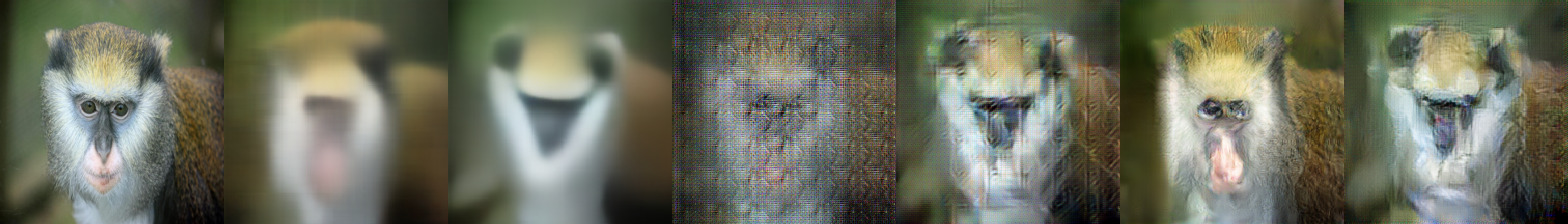
\includegraphics[width=\textwidth]{figs/ablation/ablation_tile2.jpg}

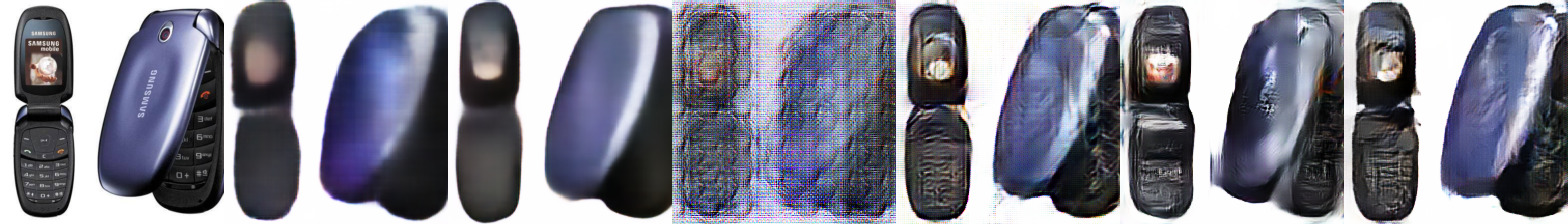
\includegraphics[width=\textwidth]{figs/ablation/ablation_tile9.jpg}

\caption{\label{fig:inversion_alexnet}AlexNet feature inversion on ImageNet. \layer{Conv5} features are inverted using our proposed generator under three different training criteria. Reconstructions from AR features are more faithful to the ground-truth image.}
\vspace{-0.4cm}
\end{figure}


We begin analyzing the reconstruction accuracy achieved by inverting features from different classifiers and empirically show that learning how to invert AR features via our proposed generator improves over standard feature inversion. Refer to \secref{sec:supp_results} and \secref{sec:supp_proposed_method} for additional inversion results and training details.

\subsection{Reconstruction Accuracy of AR Autoencoders}
\label{sec:experimental_inverting}
\textbf{Inverting AlexNet features.} Standard and AR AlexNet autoencoders are trained as described in \secref{sec:proposed_inversion} on ImageNet for comparison purposes. The AR AlexNet classifier is trained via $\ell_{2}$-PGD attacks \cite{madry_2018_towards} of radius $\varepsilon=\frac{3}{255}$ and $7$ steps of size $0.5$. Training is performed using $90$ epochs via SGD with a learning rate of $0.1$ reduced $10$ times every $30$ epochs. On the other hand, the standard AlexNet classifier is trained on natural images via cross-entropy (CE) loss with the same SGD setup as in the AR case.

Next, generators are trained  using pixel, feature and GAN losses to invert AlexNet \layer{conv5} features (size $6\times6\times256$). Both AR and standard models use the same generator architecture, which corresponds to the mirror network of the encoder. We deliberately use a simple architecture to highlight the reconstruction improvement is due to inverting AR features and not the generator capacity. We also train generators using (i) pixel and (ii) pixel and feature losses to ablate their effect. Reconstruction quality is evaluated using PSNR, SSIM and LPIPS.

Under all three loss combinations, reconstructions from AR AlexNet features obtain better PSNR and SSIM than their standard counterparts (\tabref{tab:inversion_alexnet}). Specifically, inverting AR AlexNet features gives an average PSNR improvement of over $2$ dB in all three cases. LPIPS scores also improve, except when using pixel, feature and GAN losses. Nevertheless, inverting AR features obtain a strong PSNR and SSIM improvement in this case as well. Qualitatively, inverting AR features better preserves the natural appearance in all cases, reducing the checkerboard effect and retaining sharp edges (\figref{fig:inversion_alexnet}).

\textbf{Inverting VGG features.} We extend the analysis to VGG-16 trained on ImageNet-143 and evaluate the reconstruction improvement achieved by inverting its AR features. We use the AR pre-trained classifier from the recent work by Liu et al.~\cite{liu_2018_adv} trained using $\ell_{\infty}$-PGD attacks of radius $\varepsilon=0.01$ and $10$ steps of size $\frac{1}{50}$. Training is performed using $80$ epochs via SGD with a learning rate of $0.1$ reduced $10$ times every $30$, $20$, $20$ and $10$ epochs. On the other hand, its standard version is trained on natural images via CE loss with the same SGD setup as in the AR case.

Generators are trained on pixel and feature losses to invert VGG-16 \layer{conv5\_1} features (size $14 \times 14 \times 512$). Similarly to the AlexNet analysis, generators inverting both standard and AR features correspond to the mirror network of the encoder. We evaluate the reconstruction accuracy of both models and report their level of adversarial robustness (\tabref{tab:inversion_vgg16} and \figref{fig:inversion_vgg16}).

\begin{table}[t]

\centering
\begin{minipage}{0.575\textwidth}
\fontsize{8.45}{10.45}\selectfont
\begin{center}
\vspace{-0.8 cm}
\caption{\label{tab:inversion_vgg16} AR VGG-16 \cite{liu_2018_adv} feature inversion on ImageNet. Training our generator via pixel and feature losses, reconstruction largely improves by inverting AR representations.}
\begin{tabular}{c|c|c}
\specialrule{.15em}{.05em}{.05em} 
 & Standard Model & AR Model (ours)\\
 \hline
\makecell{Standard Accuracy} & $65.0$ & $48.7$\\
\makecell{$\ell_{\infty}$ PGD Accuracy} & $0$ & $23.0$\\
\hline
\makecell{PSNR (dB) $\uparrow$} & $18.35\pm 2.471$ & $\mathbf{21.063\pm 3.132}$\\
\makecell{SSIM $\uparrow$} & $0.466\pm 0.2$ & $\mathbf{0.538\pm 0.165}$\\
\makecell{LPIPS $\downarrow$} & $0.327\pm 0.101$ & $\mathbf{0.225\pm0.057}$\\
\specialrule{.15em}{.05em}{.05em} 
\end{tabular}
\end{center}
\end{minipage}
\hfill
\begin{minipage}{0.375\textwidth}
\hspace{2.21\baselineskip}\noindent\fcolorbox{white}{white}{\begin{minipage}[t]{0.155\textwidth}
\centering\textbf{{\scalebox{0.525}{\hspace{-0.25\baselineskip}G. truth}}}
\end{minipage}}\noindent\fcolorbox{white}{white}{\begin{minipage}[t]{0.16\textwidth}
\centering\textbf{{\scalebox{0.525}{\hspace{-0.15\baselineskip}Standard}}}
\end{minipage}}\noindent\fcolorbox{white}{white}{\begin{minipage}[t]{0.15\textwidth}
\centering\textbf{{\scalebox{0.525}{\hspace{-0.55\baselineskip}AR (Ours)}}}
\end{minipage}}

\begin{center}
\vspace{-0.475cm}
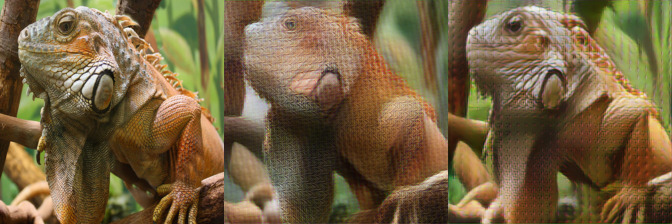
\includegraphics[width=0.63\textwidth]{figs/vgg16/rec_tile_0.jpg}

\includegraphics[width=0.63\textwidth]{figs/vgg16/rec_tile_1.jpg}

\includegraphics[width=0.63\textwidth]{figs/vgg16/rec_tile_2.jpg}
\end{center}
\captionof{figure}{\label{fig:inversion_vgg16} AR VGG-16 reconstruction on ImageNet.}
\end{minipage}
\vspace{-0.8 cm}
\end{table}


Quantitatively, reconstructions from AR VGG-16 features are more accurate than those of standard features in PSNR, SSIM and LPIPS by a large margin. Specifically, inverting AR VGG-16 features gives an average PSNR improvement of $2.7$ dB. Qualitatively, reconstructions from AR VGG-16 features are more similar to the original images, reducing artifacts and preserving object boundaries.

Furthermore, the reconstruction accuracy attained by the AR VGG-16 autoencoder improves over that of the AR AlexNet model. This suggests that the benefits of inverting AR features are not constrained to shallow models such as AlexNet, but generalize to models with larger capacity.

\textbf{Inverting ResNet features.} To analyze the effect of inverting AR features from classifiers trained on different datasets, we evaluate the reconstruction accuracy obtained by inverting WideResNet-28-10 trained on CIFAR-10. We use the AR pre-trained classifier from the recent work by Zhang et al.~\cite{zhang_2020_geometry}. This model obtains State-of-the-art AR classification accuracy via a novel weighted adversarial training regime. Specifically, the model is adversarially trained via PGD by ranking the importance of each sample based on how close it is to the decision boundary (how \textit{attackable} the sample is).

AR training is performed using $\ell_{\infty}$ attacks of radius $\varepsilon=\frac{8}{255}$ and $10$ steps of size $\frac{2}{255}$. Classification training is performed using $100$ epochs (with a burn-in period of $30$ epochs) via SGD with a learning rate of $0.1$ reduced $10$ times every $30$ epochs. On the other hand, its standard version is trained on natural images via CE loss using the same SGD setup as in the AR case.

Generators for standard and AR WideResNet-28-10 models are trained to invert features from its 3rd residual block (size $8\times 8 \times 640$) via pixel and feature losses. Similarly to our previous analysis, both generators correspond to the mirror architecture of the encoder. We evaluate their reconstruction via PSNR, SSIM and LPIPS, and their robustness via AutoAttack \cite{croce_2020_reliable} (\tabref{tab:inversion_resnet28} and \figref{fig:inversion_resnet28}).

Similarly to previous scenarios, inverting WideResNet-28-10 AR features shows a large improvement over standard ones in all metrics. Specifically, inverting AR features increases PSNR in $4.8$ dB on average over standard features. Visually, the AR WideResNet-28-10 autoencoder reduces bogus components and preserves object contours on CIFAR-10 test samples.

Overall, results enforce our claim that the \textbf{benefits of inverting AR features extend to different models, datasets and training strategies}.
\begin{table}[t]
\vspace{-0.25cm}
\centering
\begin{minipage}{0.575\textwidth}
\fontsize{8.5}{10.5}\selectfont
\begin{center}
\vspace{-0.5 cm}
\caption{\label{tab:inversion_resnet28} AR WideResNet-28-10 \cite{zhang_2020_geometry} feature inversion on CIFAR-10. Inverting AR features via our generator trained on pixel and feature losses significantly improves reconstruction.}
\begin{tabular}{c|c|c}
\specialrule{.15em}{.05em}{.05em} 
 & Standard Model & AR Model (ours)\\
\hline
\makecell{Standard Accuracy} & $93.8$ & $89.36$\\
\makecell{AutoAttack \cite{croce_2020_reliable}} & \makecell{$0$} & \makecell{$59.64$}\\
\hline
PSNR (dB) $\uparrow$ & $17.38\pm 2.039$ & $\mathbf{22.14\pm 1.626}$\\
SSIM $\uparrow$ & $0.59\pm 0.1$ & $\mathbf{0.81\pm 0.067}$ \\
LPIPS $\downarrow$ & $0.2547\pm 0.055$ & $\mathbf{0.2318\pm 0.0833}$\\
  
\specialrule{.15em}{.05em}{.05em} 
\end{tabular}
\end{center}
\end{minipage}
\hfill
\begin{minipage}{0.375\textwidth}
\vspace{0.2 cm}

\hspace{2.21\baselineskip}\noindent\fcolorbox{white}{white}{\begin{minipage}[t]{0.155\textwidth}
\centering\textbf{{\scalebox{0.525}{\hspace{-0.25\baselineskip}G. truth}}}
\end{minipage}}\noindent\fcolorbox{white}{white}{\begin{minipage}[t]{0.16\textwidth}
\centering\textbf{{\scalebox{0.525}{\hspace{-0.15\baselineskip}Standard}}}
\end{minipage}}\noindent\fcolorbox{white}{white}{\begin{minipage}[t]{0.15\textwidth}
\centering\textbf{{\scalebox{0.525}{\hspace{-0.55\baselineskip}AR (Ours)}}}
\end{minipage}}

\begin{center}
\vspace{-0.475cm}
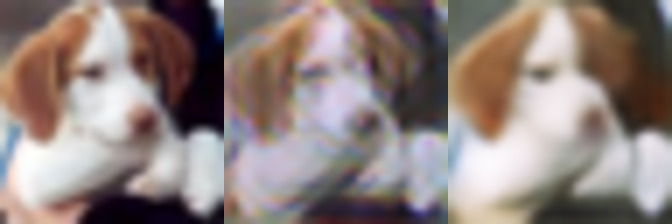
\includegraphics[width=0.63\textwidth]{figs/resnet28/rec_tile_5.jpg}

\includegraphics[width=0.63\textwidth]{figs/resnet28/rec_tile_1.jpg}

\includegraphics[width=0.63\textwidth]{figs/resnet28/rec_tile_2.jpg}
\end{center}
\captionof{figure}{\label{fig:inversion_resnet28} AR WideResNet-28-10 reconstruction on CIFAR-10.}
\end{minipage}
\vspace{-1 cm}
\end{table}



\subsection{Robustness Level vs. Reconstruction Accuracy}
\label{relationship_adversarial}
We complement the reconstruction analysis by exploring the relation between adversarial robustness and inversion quality. We train five AlexNet classifiers on ImageNet, one on natural images (standard) and four via $\ell_{2}$-PGD attacks with $\varepsilon\in \{0.5,2,3,4\}/255$. All other training parameters are identical across models.

For each classifier, an image generator is trained on an ImageNet subset via pixel, feature and GAN losses to invert \layer{conv5} features. Similar to \secref{sec:experimental_inverting}, all five generators correspond to the mirror network of the encoder. To realiably measure the impact of adversarial robustness, reconstruction accuracy is evaluated in terms of PSNR, SSIM and LPIPS. We also report the effective robustness level achieved by each model via AutoAttack (\tabref{tab:rob_vs_acc}).
\begin{table}[t]
\begin{center}
\vspace{0.3cm}
\caption{\label{tab:rob_vs_acc} Reconstruction vs. Robustness. Experiments on ImageNet show that learning to invert AlexNet features with different AR levels can significantly improve the reconstruction accuracy.}
\resizebox{0.75\columnwidth}{!}{
\begin{tabular}{c|c|c|c|c|c}
\specialrule{.15em}{.05em}{.05em}
& \multicolumn{5}{c}{$\ell_{2}$ PGD Attack ($\varepsilon$)}\\
\cline{2-6}
& $0$ & $0.5$ & $2$ & $3$ & $4$ \\
\hline
\makecell{Standard Accuracy} & $53.69$ & $49.9$ & $43.8$ & $39.83$ & $36.31$\\
\makecell{AutoAttack \cite{croce_2020_reliable}} & \makecell{$8.19$ ($\varepsilon=0.5$)} & \makecell{$48.0$ ($\varepsilon=0.5$)} & \makecell{$28.0$ ($\varepsilon=2$)} & \makecell{$22.27$ ($\varepsilon=3$)} & \makecell{$14.9$ ($\varepsilon=4$)}\\
\hline
PSNR (dB) $\uparrow$ & $13.12$ & $14.41$ & $15.5$ & ${15.53}$ & $\mathbf{15.61}$\\
SSIM $\uparrow$ & $0.20$ & $0.26$ & $\mathbf{0.3}$ & ${0.26}$ & $0.25$\\
LPIPS $\downarrow$ & $0.657$ & ${0.625}$ & $\mathbf{0.614}$ & $0.629$ & $0.644$\\
\specialrule{.15em}{.05em}{.05em} 
\end{tabular}}
\end{center}
\vspace{-0.5cm}
\end{table}

\begin{table}[t]
\centering
\setlength\tabcolsep{2pt}
\begin{minipage}{0.5\textwidth}
\begin{center}
\vspace{-0.8 cm}
\caption{\label{tab:eval_scale} Reconstructing upscaled ImageNet samples. Images upscaled by a factor $L$ are reconstructed from their standard and AR AlexNet features. In contrast to the degraded standard reconstructions, AR reconstructions show an outstanding accuracy that improves for large scaling factors.}
\vspace{0.1 cm}
\fontsize{8.5}{10.5}\selectfont
\def\arraystretch{1.25}
\resizebox{1\columnwidth}{!}{%
\begin{tabular}{c|c|c|c|c|c|c}
\specialrule{.15em}{.05em}{.05em} 
\multirow{2}{*}{\makecell{$L$}} & \multicolumn{3}{c|}{\makecell{Standard\\AlexNet}} & \multicolumn{3}{c}{\makecell{Robust\\AlexNet}} \\
\cline{2-7}
& \makecell{PSNR\\(dB)$\uparrow$} & SSIM$\uparrow$ & LPIPS$\downarrow$ & \makecell{PSNR\\(dB)$\uparrow$} & SSIM$\uparrow$ & LPIPS$\downarrow$\\
\hline
 $1$ & \makecell{$15.057$} & \makecell{$0.3067$} & \makecell{$0.5473$} & \makecell{$17.2273$} & \makecell{$0.3580$} & \makecell{$0.5665$}\\
 $4$ & \makecell{$15.4258$} & \makecell{$0.4655$} & \makecell{$0.4136$} & \makecell{$22.575$} & \makecell{$0.5892$} & \makecell{$0.4012$}\\
 $7$ & \makecell{$13.8922$} & \makecell{$0.4852$} & \makecell{$0.4587$} & \makecell{$23.5778$} & \makecell{$0.6588$} & \makecell{$0.3898$}\\
 $10$ & \makecell{$13.1013$} & \makecell{$0.4969$} & \makecell{$0.486$} & \makecell{$23.9566$} & \makecell{$0.7244$} & \makecell{$0.3892$}\\
\specialrule{.15em}{.05em}{.05em} 
\end{tabular}
}
\end{center}
\end{minipage}
\hfill
\begin{minipage}{0.475\textwidth}

\begin{minipage}{0.2\textwidth}
\centering\textbf{\colorbox{white}{\scalebox{0.68}{G. truth}}}
\end{minipage}\begin{minipage}{0.2\textwidth}
\centering \colorbox{white}{\scalebox{0.7}{$L= 1$}}
\end{minipage}\begin{minipage}{0.2\textwidth}
\centering \colorbox{white}{\scalebox{0.7}{$L= 4$}}
\end{minipage}\begin{minipage}{0.2\textwidth}
\centering \colorbox{white}{\scalebox{0.7}{$L= 7$}}
\end{minipage}\begin{minipage}{0.2\textwidth}
\centering \colorbox{white}{\scalebox{0.7}{$L= 10$}}
\end{minipage}

\vspace{-0.05 cm}
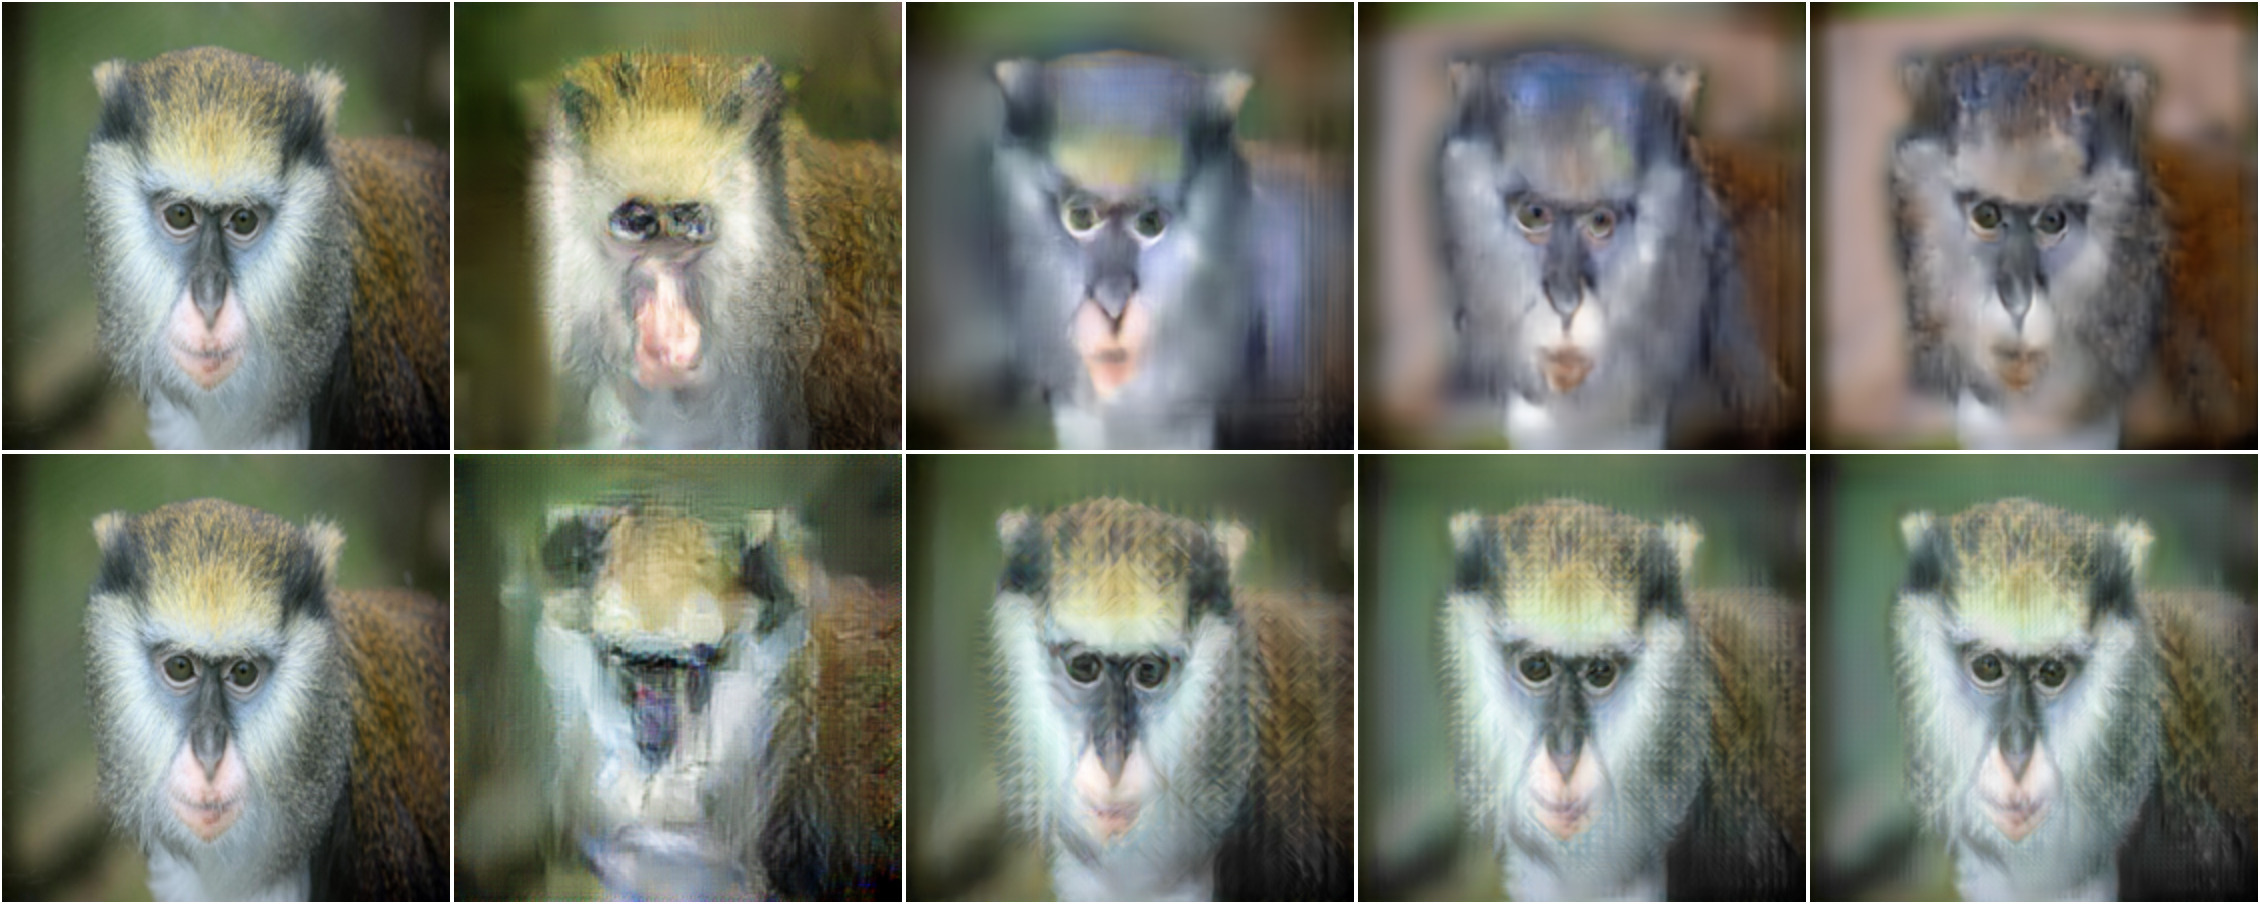
\includegraphics[width=1\textwidth]{figs/upscaling/tile_group_hires01_2.jpg}

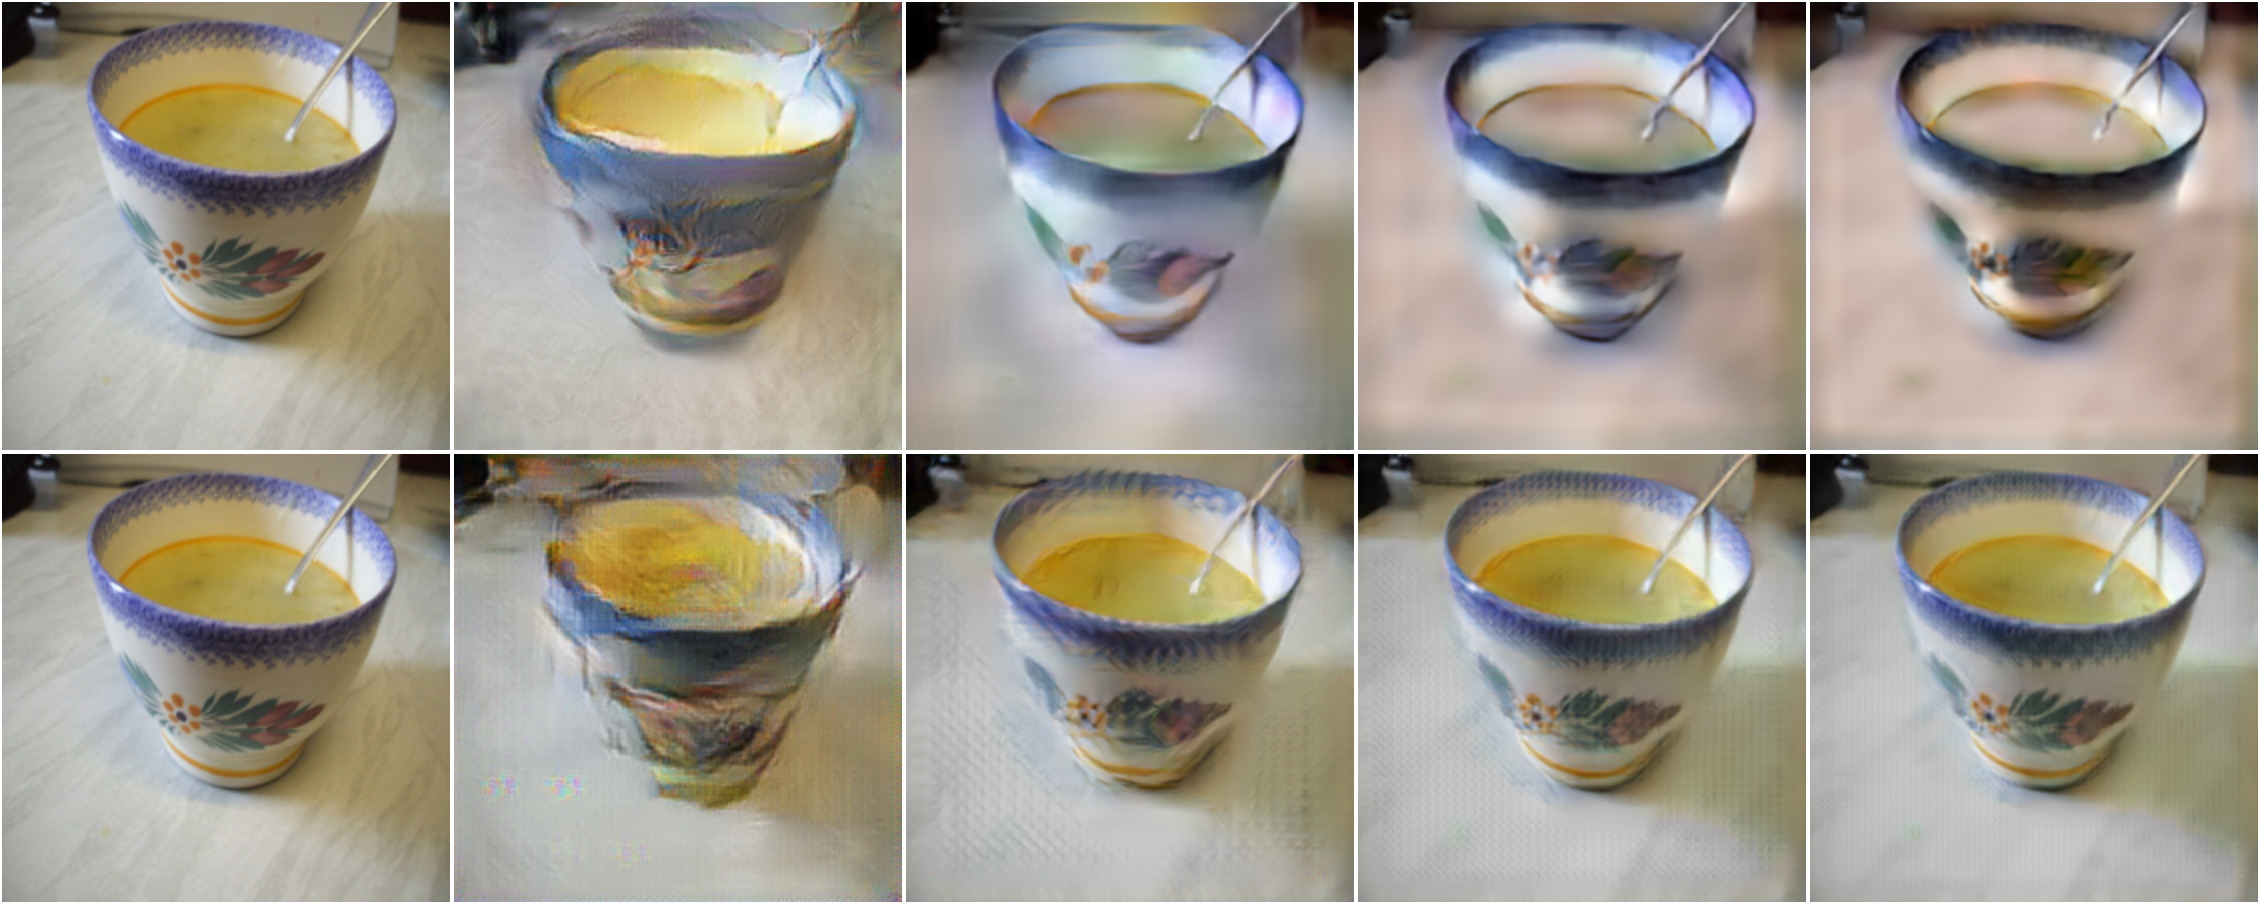
\includegraphics[width=1\textwidth]{figs/upscaling/tile_group_hires01_1.jpg}

\vspace{0.3 cm}
\captionof{figure}{\label{fig:eval_scale}Upscaled ImageNet samples reconstructed from their standard (top row) and AR (bottom row) features.}

\end{minipage}
\vspace{-0.5cm}
\end{table}


Results show LPIPS and SSIM improve almost monotonically until a maximum value is reached at $\varepsilon=2$, while PSNR keeps increasing. This implies that just by changing $\varepsilon$ from $0.5$ to $4$ while keeping the exact same architecture and training regime, a reconstruction improvement of $1.2$ dB PSNR is obtained.

Based on this, we use an AR AlexNet model trained with $\varepsilon=3$ in our experiments, which gives the best tradeoff between PSNR, SSIM and LPIPS. Overall, our analysis suggests that, while all four AR models outperform the inversion accuracy of the standard model, the reconstruction improvement is not proportional to the robustness level. Instead, it is maximized at a particular level. Please refer to \secref{sec:supp_inverting_alternative} for additional robustness level vs. reconstruction accuracy experiments on ResNet-18 pointing to the same conclusion.

\subsection{Reconstructing Images at Unseen Resolutions}
\label{sec:experimental_scale}

Unlike extracting shift-invariant representations, image scaling is difficult to handle for standard CNN-based models \cite{sosnovik_2019_scale,fan_2020_scale}. Following previous work suggesting AR features are more generic and transferable than standard ones \cite{chen2020shape,salman_2020_adversarially}, we test whether our proposed AR autoencoder generalizes better to scale changes. We explore this property and show that our model trained on low-resolution samples improves reconstruction of images at unseen scales without any fine-tuning.

\textbf{Scenario 1: Reconstructing Upscaled Images.} Upscaled ImageNet samples are reconstructed from their AR AlexNet \layer{conv5} representations. For a fair comparison across scales, each image is normalized to $224 \times 224$ px. and then enlarged by an integer factor $L>1$. Experiments show a higher accuracy obtained from AR features in terms of PSNR, SSIM and LPIPS (\tabref{tab:eval_scale}). All metrics improve almost monotonically with $L$. In contrast, accuracy using standard features degrades with $L$.
Inversion from AR features show almost perfect reconstruction for large scales, while those of standard features show severe distorsions (\figref{fig:eval_scale}).

\begin{table}[bpt!]
\begin{center}
\vspace{-0.2 cm}
\caption{\label{tab:hires} High-resolution images inverted using our AR AlexNet model (trained on low resolution images) show improved quality over standard inversions.}
\vspace{0.1 cm}
\fontsize{8.5}{10.5}\selectfont
\setlength\tabcolsep{2pt}
\resizebox{0.75\columnwidth}{!}{
\begin{tabular}{c|c|c|c} 
\specialrule{.15em}{.05em}{.05em} 
\makecell{Encoder} & PSNR (dB)$\uparrow$ & SSIM$\uparrow$ & LPIPS$\downarrow$\\
\hline
 Standard & \makecell{$14.266\pm$ $1.9015$} & \makecell{$0.3874\pm$ $0.151$} & \makecell{$0.5729\pm$ $0.0465$}\\
 AR (ours) & \makecell{$\mathbf{18.3606\pm}$ $\mathbf{2.6012}$} & \makecell{$\mathbf{0.4388\pm}$ $\mathbf{0.1508}$} & \makecell{$\mathbf{0.5673\pm}$ $\mathbf{0.0337}$}\\
\specialrule{.15em}{.05em}{.05em} 
\end{tabular}
}
\end{center}
\vspace{-0.625 cm}
\end{table}

\begin{figure}[t]
\begin{minipage}[t]{0.166\textwidth}
\centering\textbf{\colorbox{white}{\scalebox{.8}{Ground-truth}}}
\end{minipage}\begin{minipage}[t]{0.166\textwidth}
\centering \textbf{\colorbox{white}{\scalebox{.8}{Standard}}}
\end{minipage}\begin{minipage}[t]{0.1725\textwidth}
\centering \textbf{\colorbox{white}{\scalebox{.8}{AR (Ours)}}}
\end{minipage}\begin{minipage}[t]{0.166\textwidth}
\centering\textbf{\colorbox{white}{\scalebox{.8}{Ground-truth}}}
\end{minipage}\begin{minipage}[t]{0.166\textwidth}
\centering \textbf{\colorbox{white}{\scalebox{.8}{Standard}}}
\end{minipage}\begin{minipage}[t]{0.166\textwidth}
\centering \textbf{\colorbox{white}{\scalebox{.8}{AR (Ours)}}}
\end{minipage}

\vspace{-0.1 cm}    
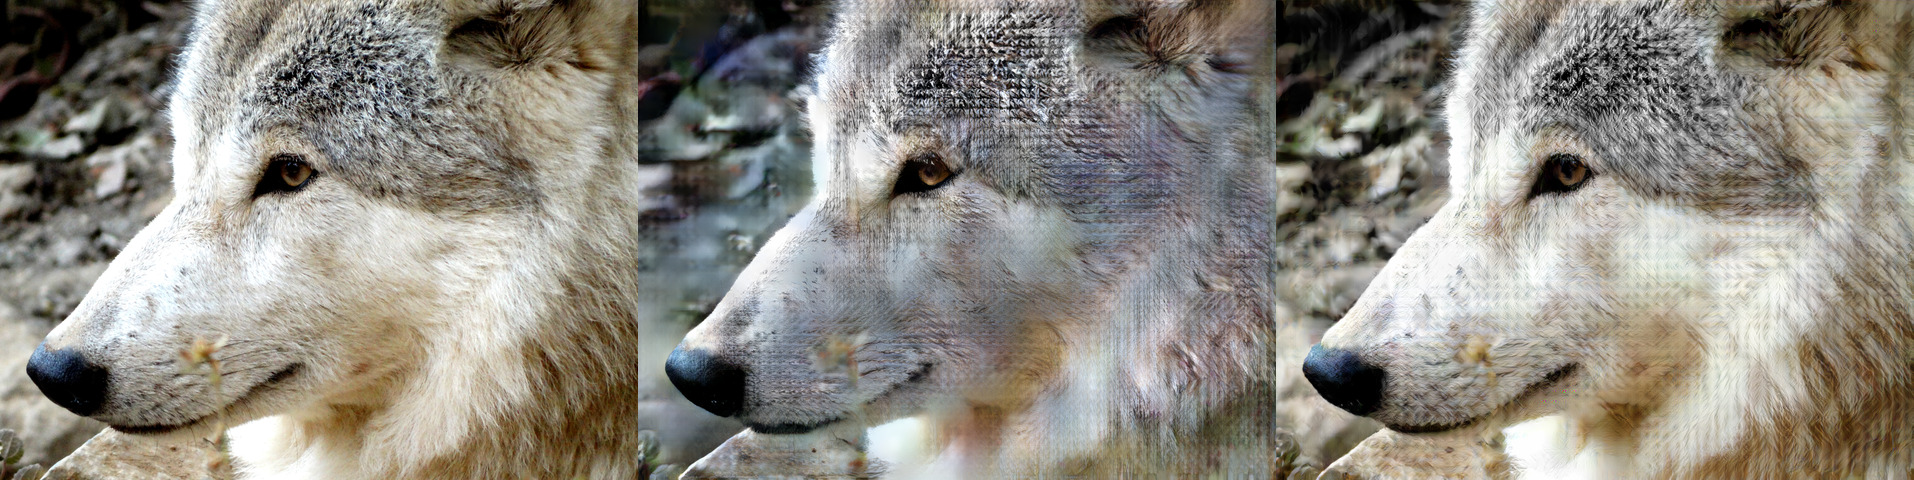
\includegraphics[width=0.5\textwidth]{figs/hires/tile_hires01_7.jpg}
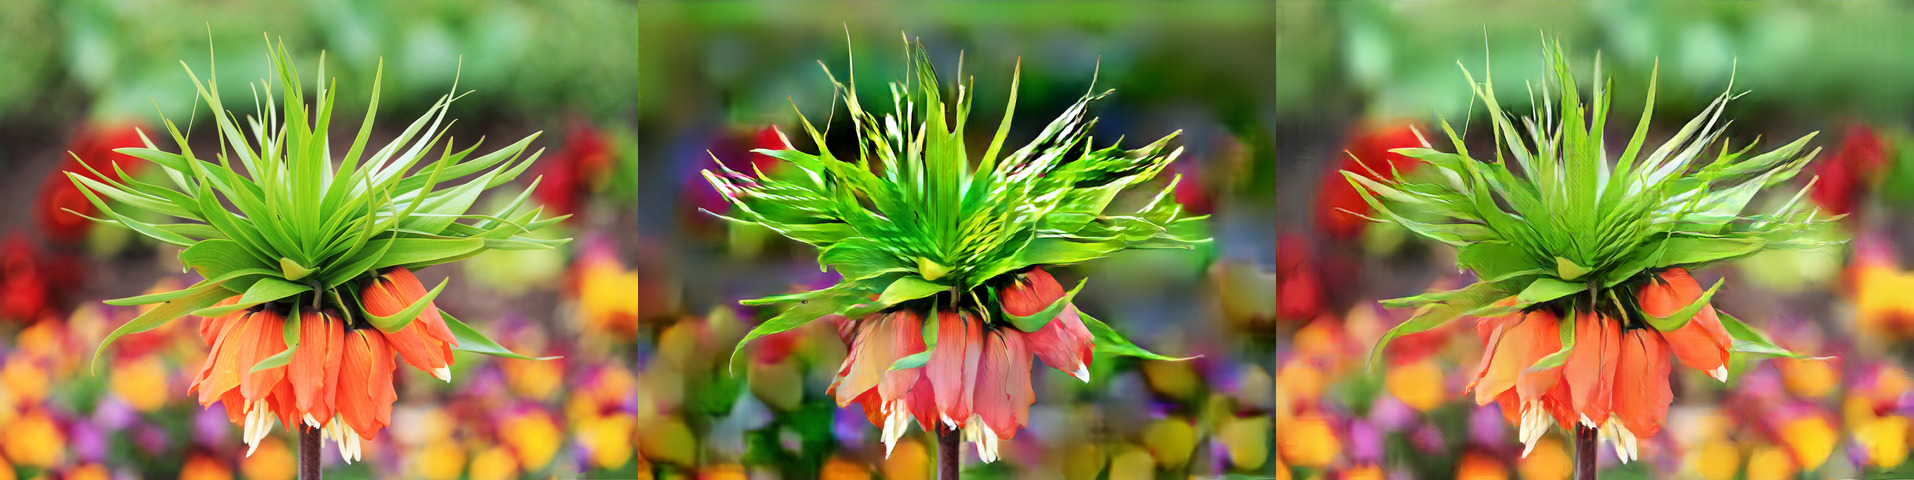
\includegraphics[width=0.5\textwidth]{figs/hires/tile_hires01_5.jpg}

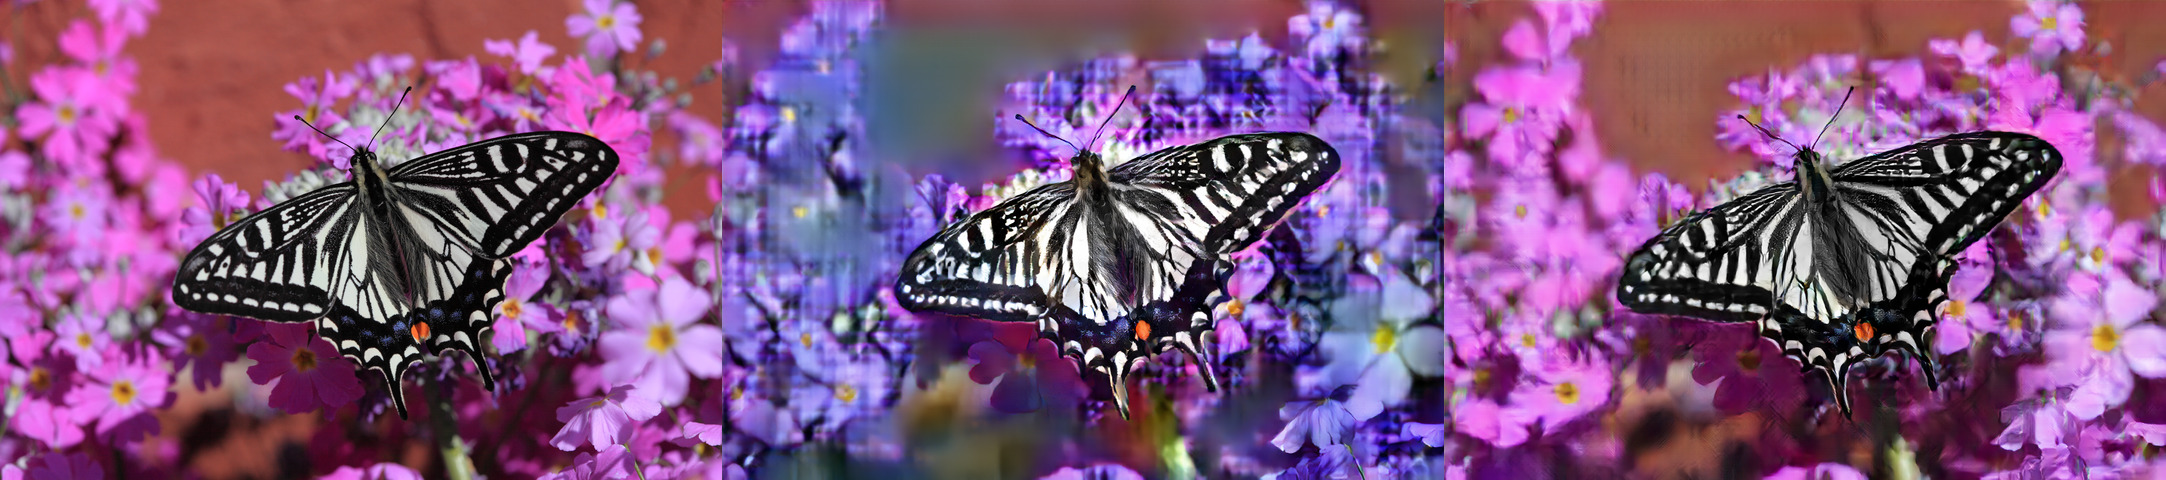
\includegraphics[width=0.5\textwidth]{figs/hires/tile_hires01_10.jpg}
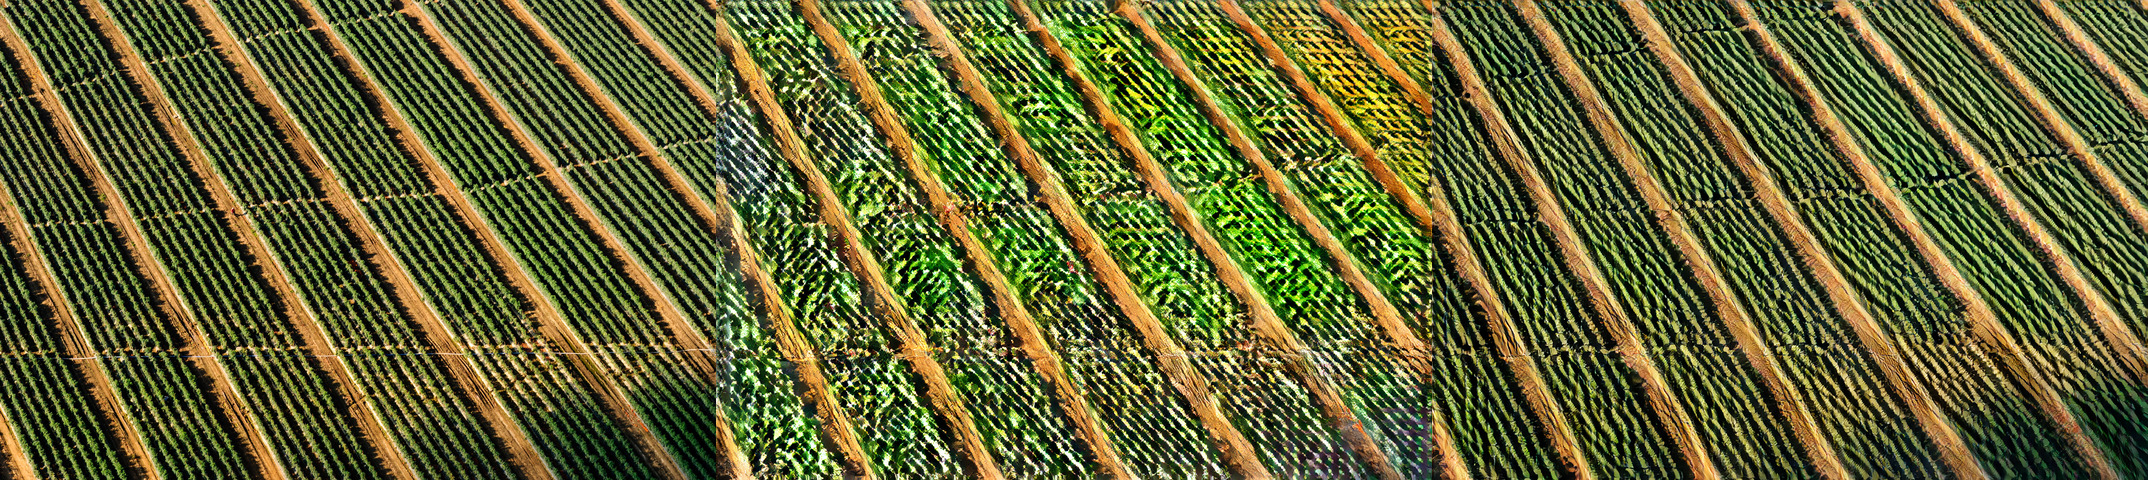
\includegraphics[width=0.5\textwidth]{figs/hires/tile_hires01_11.jpg}

\vspace{-0.1 cm}
\caption{\label{fig:hires}At a resolution of $2040\times 1536$ px., $10$ times larger than training samples, standard reconstructions on DIV2K show color and structure degradation. In contrast, reconstructions from our AR model do not suffer from distortions.}
\vspace{-0.5 cm}
\end{figure}


\textbf{Scenario 2: Reconstructing High-Resolution Images.} Standard and AR feature inversion is performed on the DIVerse 2K resolution dataset (DIV2K) \cite{agustsson_2017_ntire}, containing objects at multiple scales. AR feature reconstructions show a significant PSNR, SSIM and LPIPS improvement over standard ones, despite not being explicitly trained to handle such large-scale objects (\tabref{tab:hires}).

Qualitatively, reconstructions from AR AlexNet features preserve sharp edges, reduces color degradation and diminishes checkerboard effects induced by standard inversion (\figref{fig:hires}). Thus, for unseen scales and without finetuning, AR features better preserve structure without penalizing the perceptual similarity.

\subsection{Comparison against State-of-the-Art Inversion Techniques}
\label{sec:experimental_comparison}
The inversion accuracy of our AR autoencoder is compared against two alternative techniques: Optimization-based robust representation inversion (RI) \cite{engstrom_2019_adversarial} and DeePSiM \cite{dosovitskiy_2015_inverting}. For a fair comparison, all methods reconstruct images from AlexNet features. We begin by highlighting the differences between them.

While RI is a model-based approach that searches in the pixel domain for an image that matches a set of target AR features, we use a CNN-based generator trained on a combination of natural-image priors (\secref{sec:opt_crit}). On the other hand, while DeePSiM is also a CNN-based technique trained under multiple priors, its generator has approximately $63\%$ more trainable parameters than ours (\tabref{tab:inversion_comparison}).

\textbf{Experimental Setup.} All inversion methods are evaluated on ImageNet. Our standard and AR models are trained using pixel, feature and GAN losses using the training setup described in \secref{sec:supp_proposed_method}. DeePSiM is evaluated using its official Caffe implementation without any changes. RI is evaluated using its official PyTorch implementation modified to invert \layer{conv5} AR features. Input samples are rescaled to $224 \times 224$ px. ($227 \times 227$ px. for DeepSiM).

\textbf{Results.} Our AR AlexNet autoencoder obtains the best accuracy in terms of PSNR and the second best in terms of SSIM (\tabref{tab:inversion_comparison}). While it outperforms its standard version in PSNR and SSIM, it gets a marginally worse LPIPS. Moreover, our AR model outperforms RI in all metrics. Also, despite DeePSiM having more layers and using larger inputs, our model achieves a large PSNR improvement over it. Results highlight the improvement obtained by inverting AR features and how this fundamental change allows competitive reconstruction quality using three times less trainable parameters.

\begin{table}[t]
\centering
\vspace{-0.3cm}
\caption{\label{tab:inversion_comparison} Comparison against state-of-the-art inversion techniques. By inverting AR features, our autoencoder outperforms the optimization-based RI method by a large margin. Despite having 63\% less parameters, we also obtain favorable results against DeepSiM, showing a significant PSNR improvement.}%
\vspace{0.1 cm}
\resizebox{\columnwidth}{!}{

\begin{tabular}{c|c|c|c|c|c}
\specialrule{.15em}{.05em}{.05em} 
Algorithm & Encoder & Trainable Pars. & PSNR (dB)$\uparrow$ & SSIM$\uparrow$ & LPIPS$\downarrow$ \\
\hline
\makecell{RI \cite{engstrom_2019_adversarial}} & \makecell{AR AlexNet} & $-$ & $16.724\pm 2.434$ & $0.181\pm 0.071$ & $0.63\pm 0.04$\\
\makecell{Standard Autoencoder} & \makecell{Standard AlexNet} & $4,696,026$ & $15.057\pm 2.392$ & $0.307\pm 0.158$ & $\mathbf{0.547\pm 0.055}$\\
\makecell{AR Autoencoder (ours)} & \makecell{AR AlexNet} & $4,696,026$ & $\mathbf{17.227\pm 2.725}$ & $\mathbf{0.358\pm 0.163}$ & $0.567\pm 0.056$\\
\hline\hline
\makecell{DeepSiM \cite{dosovitskiy_2016_generating}} & \makecell{Standard CaffeNet} & $12,702,307$ & $15.321\pm 2.011$ & $0.417\pm 0.158$ & $0.531\pm 0.059$\\
\specialrule{.15em}{.05em}{.05em} 
\end{tabular}}
\vspace{-0.55 cm}
\end{table}


\bibliography{main.bib}
\bibliographystyle{theapa}
\clearpage
\appendix
\section{Probability Lemma and Concentration Bounds} \label{apx:prob}
\begin{lemma}\label{lemma:chernoff}
    (Chernoff bounds \cite{mitzenmacher2017probability}). 
    Suppose $X_1$, ... , $X_n$ are independent binary random variables such that 
    $\prob{X_i = 1} = p_i$. Let $\mu = \sum_{i=1}^n p_i$, and 
    $X = \sum_{i=1}^n X_i$. Then for any $\delta \geq 0$, we have
    \begin{align}
        \prob{X \ge (1+\delta)\mu} \le e^{-\frac{\delta^2 \mu}{2+\delta}}.
    \end{align}
    Moreover, for any $0 \leq \delta \leq 1$, we have
    \begin{align}
        \prob{X \le (1-\delta)\mu} \le e^{-\frac{\delta^2 \mu}{2}}.
    \end{align}
\end{lemma}
\begin{lemma} \label{lemma:indep}
    \cite{chen2021best}.
    Suppose there is a sequence of $n$ Bernoulli trials:
    $X_1, X_2, \ldots, X_n,$
    where the success probability of $X_i$
    depends on the results of
    the preceding trials $X_1, \ldots, X_{i-1}$.
    Suppose it holds that $$\prob{X_i = 1 | X_1 = x_1, X_2 = x_2, \ldots, X_{i-1} = x_{i-1} } \ge \eta,$$ where $\eta > 0$ is a constant and $x_1,\ldots,x_{i-1}$ are arbitrary.
  
    Then, if $Y_1,\ldots, Y_n$ are independent Bernoulli trials, each with probability $\eta$ of
    success, then $$\prob {\sum_{i = 1}^n X_i \le b } \le \prob{\sum_{i = 1}^n Y_i \le b }, $$
    where $b$ is an arbitrary integer.
  
    Moreover, let $A$ be the first occurrence of success in sequence $X_i$.
    Then, $$\ex{A} \le 1/\eta.$$
\end{lemma}
\begin{lemma} \label{lemma:indep2}
    \cite{chen2021best}.
    Suppose there is a sequence of $n+1$ Bernoulli trials:
    $X_1, X_2, \ldots,X_{n+1},$
    where the success probability of $X_i$
    depends on the results of
    the preceding trials $X_1, \ldots, X_{i-1}$,
    and it decreases from 1 to 0.
    Let $t$ be a random variable based on the $n+1$ Bernoulli trials.
    Suppose it holds that 
    $$\prob{X_i = 1 | X_1 = x_1, X_2 = x_2, \ldots, X_{i-1} = x_{i-1}, i\le t } \ge \eta,$$ 
    where $x_1,\ldots,x_{i-1}$ are arbitrary and $0 < \eta < 1$ is a constant.
    Then, if $Y_1,\ldots, Y_{n+1}$ are independent Bernoulli trials, each with probability $\eta$ of
    success, then 
    $$\prob {\sum_{i = 1}^t X_i \le bt } \le \prob{\sum_{i = 1}^t Y_i \le bt }, $$
    where $b$ is an arbitrary integer.
\end{lemma}
% \begin{proof}
%   Let $Z_j=\sum_{i=1}^j X_i \cdot 1_{\{i\le t\}} + \sum_{i=j+1}^{n+1} Y_i \cdot 1_{\{i\le t\}}$,
%   where $$Z_0=\sum_{i=1}^{n+1} Y_i \cdot 1_{\{i\le t\}} = \sum_{i = 1}^t Y_i$$
%   and $$Z_{n+1}=\sum_{i=1}^{n+1} X_i \cdot 1_{\{i\le t\}} = \sum_{i = 1}^t X_i.$$
%   If for any $1\le j \le n+1$, 
%   \begin{equation} \label{ineq:seq}
%     \prob{Z_j \le bt} \le 
%   \prob{Z_{j-1} \le bt},
%   \end{equation}
%   then,
%   $$\prob{Z_{n+1} \le bt} \le
%   \prob{Z_0 \le bt}.$$

%   In the following, we will prove Inequality~\ref{ineq:seq}.
%   \begin{align*}
%     &\prob{Z_j \le bt}\\
%     &= \prob{X_j\cdot 1_{\{j\le t\}}=0, Z_j-X_j\cdot 1_{\{j\le t\}} \le bt-1}\\
%     & \quad +\prob{X_j\cdot 1_{\{j\le t\}}=1, Z_j-X_j\cdot 1_{\{j\le t\}} \le bt-1}\\
%     & \quad +\prob{X_j\cdot 1_{\{j\le t\}}=0, Z_j-X_j\cdot 1_{\{j\le t\}} = bt}\\
%     &= \prob{Z_j-X_j\cdot 1_{\{j\le t\}} \le bt-1}\\
%     &\quad + \prob{1_{\{j\le t\}}=0,Z_j-X_j\cdot 1_{\{j\le t\}} = bt}\\
%     &\quad + \prob{X_j=0,1_{\{j\le t\}}=1,Z_j-X_j\cdot 1_{\{j\le t\}} = bt}\\
%     &= \prob{Z_j-X_j\cdot 1_{\{j\le t\}} \le bt-1}\\
%     &\quad + \prob{1_{\{j\le t\}}=0,Z_j-X_j\cdot 1_{\{j\le t\}} = bt}\\
%     &\quad + \sum_{Z_j-X_j\cdot 1_{\{j\le t\}} = bt,j\le t}
%     \prob{X_j=0 | X_1,\cdots, X_{j-1},Y_{j+1},\cdots, Y_{n+1}, j\le t} \\
%     &\quad \cdot \prob{X_1,\cdots, X_{j-1},Y_{j+1},\cdots, Y_{n+1}, j\le t}\\
%     &\le \prob{Z_j-X_j\cdot 1_{\{j\le t\}} \le bt-1}\\
%     &\quad + \prob{1_{\{j\le t\}}=0,Z_j-X_j\cdot 1_{\{j\le t\}} = bt}\\
%     &\quad + \sum_{Z_j-X_j\cdot 1_{\{j\le t\}} = bt,j\le t}
%     \prob{Y_j=0}\cdot \prob{X_1,\cdots, X_{j-1},Y_{j+1},\cdots, Y_{n+1}, j\le t}\\
%     &= \prob{Z_j-X_j\cdot 1_{\{j\le t\}} \le bt-1}\\
%     &\quad + \prob{1_{\{j\le t\}}=0,Z_j-X_j\cdot 1_{\{j\le t\}} = bt}\\
%     &\quad + \prob{Y_j=0,1_{\{j \le t\}}=1,Z_j-X_j\cdot 1_{\{j\le t\}} = bt}\\
%     &= \prob{Z_j-X_j\cdot 1_{\{j\le t\}} \le bt-1}\\
%     &\quad + \prob{Y_j\cdot 1_{\{j\le t\}}=0,Z_j-X_j\cdot 1_{\{j\le t\}} = bt}\\
%     &= \prob{Z_{j-1}\le bt}.
%   \end{align*}
% \end{proof}
% \begin{lemma}\label{lemma:comb}
%     Given $n=2m$ and $t\le n$, it holds that,
%     \[\sum_{j=\max\{0, t-m\}}^{\lfloor t/2\rfloor}
%     (t-2j)\cdot C_m^i \cdot C_{m-i}^{t-2i}\cdot 2^{t-2i}
%     =n\cdot C_{n-2}^{t-1}.\]
% \end{lemma}
% \begin{proof}
%     We construct a function $F(x,y)=(x^2+2xy+1)^m$ and
%     expand it by the power of $x$ as follows,
%     \[F(x,y)=(x^2+2xy+1)^m = \sum_{t=0}^{n}\left(\sum_{j=\max\{0, t-m\}}^{\lfloor t/2\rfloor}
%     C_m^i \cdot C_{m-i}^{t-2i} \cdot (2y)^{t-2i}\right)x^t.\]
%     Then we calculate the partial derivative of $F$ with respect to $y$
%     based on the above two variants of $F$,
%     \[\frac{\partial F(x,y)}{\partial y}=nx(x^2+2xy+1)^{m-1}
%     =\sum_{t=0}^{n}\left(\sum_{j=\max\{0, t-m\}}^{\lfloor t/2\rfloor}
%     C_m^i \cdot C_{m-i}^{t-2i}\cdot 2^{t-2i}\cdot (t-2i)\cdot y^{t-2i-1}\right)x^t.\]
%     Set $y=1$,
%     \[\left. \frac{\partial F(x,y)}{\partial y}\right|_{y=1}=nx(x+1)^{n-2}
%     =\sum_{t=0}^{n}\left(\sum_{j=\max\{0, t-m\}}^{\lfloor t/2\rfloor}
%     C_m^i \cdot C_{m-i}^{t-2i}\cdot 2^{t-2i}\cdot (t-2i)\right)x^t.\]
%     Then, with $(x+1)^{n-2}=\sum_{t=0}^{n-2}C_{n-2}^t \cdot x^t$, it holds that,
%     \[\sum_{j=\max\{0, t-m\}}^{\lfloor t/2\rfloor}
%     C_m^i \cdot C_{m-i}^{t-2i}\cdot 2^{t-2i}\cdot (t-2i)
%     =n \cdot C_{n-2}^{t-1}.\]
% \end{proof}
\section{Counterexample for \thresam with Non-monotone Submodular Functions}
\label{sec:counterexample}
\shortciteS{Fahrbach2018} proposed a subroutine, 
\thresam, which returns a solution
$S \subseteq \mathcal{N}$ that $\ex{f(S)/S} \ge (1-\epsi)\tau$
within logarithmic rounds and linear time. 
The full pseudocode for \thresam is given in Alg.~\ref{alg:thresh}.
The notation $\mathcal U ( S, t )$ represents the uniform distribution 
over subsets of $S$ of size $t$. 
\thresam relies upon the procedure \reducedmean, given in Alg.~\ref{alg:rm}.
The Bernoulli distribution input to \reducedmean is the distribution 
$\mathcal D_t$, which is defined as follows. 
\begin{definition} \label{def:indicator}
  Conditioned on the current state of the algorithm,
  consider the process where the set $T \sim \mathcal U (A, t - 1)$ and then
  the element $x \sim A \setminus T$ are drawn uniformly at random.
  Let $\mathcal D_t$ denote the probability distribution over the indicator
  random variable 
  $$I_t = \mathbb I [f( S \cup T  + x) - f( S \cup T ) \ge \tau ]. $$
\end{definition}

Below, we state the lemma of \thresam in \shortciteS{Fahrbach2018}.
\begin{lemma}[\citeS{Fahrbach2018}] \label{lemm:thresh} 
  The algorithm \thresam outputs $S \subseteq \mathcal N$ with
  $|S| \le k$ in $O( \log (n / \delta ) / \epsi )$ adaptive
  rounds such that the following properties hold with 
  probability at least $1 - \delta$: 
  \begin{itemize}
    \item[1.] There are $O( n / \epsi )$ oracle queries in expectation.
    \item[2.] The expected average marginal $\ex{f(S)/|S|} \ge (1-\epsi)\tau$.
    \item[3.]  If $|S| < k$, then $f_x(S) < \tau$ for all 
    $x \in \mathcal N$.
  \end{itemize}
\end{lemma}

In \shortciteS{Fahrbach2018a} and \shortciteS{kuhnle2021nearly},
the above Lemma is used with non-monotone submodular functions;
however, in the case that $f$ is non-monotone, the lemma does not hold.
Alg.~\ref{alg:rm} only checks (on Line \ref{line:Check}) if there is 
more than a constant fraction of 
elements whose marginal gains are larger than the threshold $\tau$.
If there exist elements with
large magnitude, \textit{negative} marginal gains, then
the average marginal gain may fail to satisfy
the lower bound in Lemma~\ref{lemm:thresh}.
As for the proof in \shortciteS{Fahrbach2018a},
the following inequality does not hold (needed for the proof of Lemma
3.3 of \shortciteS{Fahrbach2018a}):
\[\ex{\marge{T}{S}}\ge (\ex{I_1}+\ex{I_2} +\ldots +\ex{I_t})\tau,\]
where $|T| = t^*$ and $t\ge t^*/(1+\hat{\epsi})$.
Next, we give a counterexample for the two versions of \thresam used in 
\shortciteS{Fahrbach2018} and \shortciteS{Fahrbach2018a} 
where the only difference is that
the if condition in Alg.~\ref{alg:thresh}
on Line~\ref{line:stopWithA} changes to $|A|<3k$
in \shortciteS{Fahrbach2018a}.
\begin{algorithm}[t] 
  \caption{The \reducedmean algorithm of \shortciteS{Fahrbach2018}} \label{alg:rm}
  \begin{algorithmic}[1]
  \State \textbf{Input:} access to a Bernoulli distribution $\mathcal D$,
 error $\epsi$, failure probability $\delta$
 \State Set number of samples $m \gets 16 \lceil \log (2 / \delta ) / \epsi^2 \rceil$
 \State Sample $X_1, X_2, \ldots, X_m \sim \mathcal D$
 \State Set $\bar \mu \gets \frac{1}{m} \sum_{i = 1}^m X_i$
 \If{ $\bar \mu \le 1 - 1.5 \epsi$ }
 \State \textbf{return} \texttt{true}
 \EndIf
 \State \textbf{return} \texttt{false}
 \end{algorithmic}
 \end{algorithm}
 \begin{algorithm}[t]
  \caption{The threshold sampling algorithm of \shortciteS{Fahrbach2018}}
  \label{alg:thresh}
  \begin{algorithmic}[1]
    \Procedure{\thresam}{$f, k, \tau, \epsi,\delta$}
    \State \textbf{Input:} evaluation oracle $f:2^{\mathcal N} \to \reals$, constraint $k$,
    threshold $\tau$, error $\epsi$, failure probability $\delta$
    \State Set smaller error $\hat{\epsi} \gets \epsi / 3$
    \State Set iteration bounds $r \gets \lceil \log_{(1 - \hat \epsi)^{-1}}(2n / \delta) \rceil, m \gets \lceil \log(k) / \hat \epsi \rceil$
    \State Set smaller failure probability $\hat \delta \gets \delta / (2r(m + 1))$
    \State Initialize $S \gets \emptyset, A \gets N$
    \For{ $r$ sequential rounds }
    \State Filter $A \gets \{ x \in A : \Delta (x, S) \ge \tau \}$\label{line:filter}
    \If{$|A| = 0$}\label{line:stopWithA}
    \State \textbf{break}
    \EndIf
    \For{$i = 0$ to $m$ in parallel}\label{thresh:for}
    \State Set $t \gets \min \{ \lfloor (1 + \hat \epsi)^i \rfloor, |A|\}$
    \State $rm[t] \gets $\reducedmean $( \mathcal D_t, \hat \epsi, \hat \delta )$ \label{line:Check}
    \EndFor
    \State $t' \gets \min t$ such that $rm[t]$ is \texttt{true}
    \State Sample $T \sim \mathcal U \left( A, \min \{t', k - |S| \} \right)$
    \State Update $S \gets S \cup T$
    \If{ $|S| = k$ }
    \State \textbf{break}
    \EndIf
    \EndFor
    \State \textbf{return} $S$
    \EndProcedure
\end{algorithmic}
\end{algorithm}

% \textbf{Counterexample 1.}
% Let $|\mathcal{N}|=15$, and for any $B \subseteq \mathcal{N}$,
% % $f(B) = 5-\left||B|-5 \right|$.
% \begin{equation*}
%   f(B)= \left\{
%     \begin{aligned}
%       &|B|,&|B| \le 12\\
%       &60-4|B|, &|B| \ge 13
%     \end{aligned}
%   \right. .
% \end{equation*}
% Run $\thresam(f, k=15, \tau=1, \epsi=0.3, \delta=0.1)$.
% \begin{proof}
%   For any $B \subseteq \mathcal{N}$ and $x\in \mathcal{N} \backslash B$, 
%   the above set function follows that
%   \begin{equation*}
%     \marge{x}{B}= \left\{
%       \begin{aligned}
%         &1&, |B| \le 11\\
%         &-4 &, |B| \ge 12
%       \end{aligned}
%     \right. ,
%   \end{equation*}
%   which means that $f$ is a non-monotone submodular function.

%   With the input value of $k$, $\tau$, $\epsi$ and $\delta$, 
%   we can get that $r=55,m=28$.
%   There are 55 rounds of the outer \textbf{for} loop,
%   and $t$ is selected from $\{1,2,\ldots, 11,13,14\}$ in the inner for loop.
%   At the first round, after filtering, it holds that $A=\mathcal{N}$.
%   When $t\le 11$, since $\marge{x}{B}=1$ with $|B|\le 11$,
%   random sampling in \textsc{Reduced-Mean} always samples 1,
%   which makes \textsc{Reduced-Mean} returns a \texttt{false}.
%   When $t=13$, since $\marge{x}{B}=-4$ with $|B| =12$,
%   random sampling in \textsc{Reduced-Mean} always samples 0.
%   In this case, it will always return a \texttt{true}.
%   Therefore, $t'=13$ in the first iteration of the outer for loop,
%   and we sample 13 elements from $A$ to $S$.
%   At the second round, all the elements in $A$ will be filtered out,
%   since, for any $x \in \mathcal{N}$, it holds that $\marge{x}{S}=-4 < 0$.
%   \textsc{Threshold-Sampling} algorithm terminates here
%   and returns a set $S$ with 13 elements.

%   In this example, we will always return a set $S$ that $|S|=13$ and $f(S)=8$.
%   But $\ex{f(S)/|S|}=8/13 < (1-\epsi)\tau=0.7$.
% \end{proof}

% \textbf{Counterexample 2.}
% For $m$ submodular functions $\{g_i: 2^{\mathcal{N}_i} \to \reals\} _{i=1}^m$,
% where $|\mathcal{N}_i| = 2$ for any $i$,
% suppose that for any $i$ and $B \subseteq \mathcal{N}_i$,
% $g_i(B) = 1-||B|-1|$.
% Define a submodular function $f: 2^{\mathcal{N}} \to \reals$ with 
% $\mathcal{N} = \bigcup_{i=1}^m \mathcal{N}_i$ as follows,
% for any $B \subseteq \mathcal{N}$, 
% $f(B)=\sum_{i=1}^m g_i(B \cap \mathcal{N}_i)$.
% Run $\thresam(f, k=, \tau=1, \epsi=, \delta=)$.
% % \begin{equation*} 
% %   f(B)= \left\{
% %     \begin{aligned}
% %       &1-||B|-1|&, \text{if } B \subseteq \mathcal{N}_i\\
% %       &\sum_{i=1}^m f(B \cap \mathcal{N}_i)&, \text{otherwise}
% %     \end{aligned}
% %   \right. .
% % \end{equation*}
% \begin{proof}
%   Fisrt, we prove that $f$ is a non-monotone submodular function.
%   Obviously, $g_i$ is a non-monotone submodular function for any $i$,
%   and $f$ is a non-monotone set function.
%   Then, for any $S \subseteq \mathcal{N}$ and $T \subseteq \mathcal{N}$,
%   \begin{align*}
%     f(S) + f(T) &= \sum_{i=1}^m \left( g_i(S \cap \mathcal{N}_i)
%     +g_i(T \cap \mathcal{N}_i)\right)\\
%     &\ge \sum_{i=1}^m \left( g_i((S \cap T)\cap \mathcal{N}_i)
%     +g_i((S\cup T) \cap \mathcal{N}_i)\right)\\
%     &= f(S \cap T) + f(S \cup T).
%   \end{align*}
%   Therefore, $f$ is a non-monotone submodular function.

%   Next, we provide the following lemma.
%   \begin{lemma}
%     Within the first round of \thresam,
%     it holds that,
%     \[\ex{I_t} = \ex{f(S)/|S|} =  \frac{n-t}{n-1},\]
%     where $I_t$ is defined in Definition~\ref{def:indicator},
%     $S \subseteq \mathcal{N}$ and $|S| = t$.
%   \end{lemma}
%   \begin{proof}
%     With Definition~\ref{def:indicator} and $\tau=1$,
%     $I_t = 1$ if and only if $\marge{x}{T}=1$, where $|T|=t-1$.
%     Without loss of generality, we assume that $x \in \mathcal{N}_1$.
%     To have that $\marge{x}{T}=1$, $x$ can be either one in $\mathcal{N}_1$,
%     and $T$ is selected from $\mathcal{N} \backslash \mathcal{N}_1$.
%     Then we can calculate $\ex{I_t}$ as follows,
%     \[\ex{I_t} = \frac{2 \cdot C_{n-2}^{t-1}}{2 \cdot C_{n-1}^{t-1}}=\frac{n-t}{n-1}.\]

%     By the definition of $f$, the objective value of $S$ is the number of 
%     $\mathcal{N}_i$ where $|S \cap \mathcal{N}_i|=1$.
%     Let $j$ be the number of $\mathcal{N}_i$ where $|S \cap \mathcal{N}_i|=2$.
%     Then $f(S) = t-2j$, where $\max\{0, t-m\} \le j \le \lfloor t/2\rfloor$. 
%     The expectation of objective value of $S$ can be calculated by
%     considering the possible combinations 
%     among the $m$ sets where there are $j$ sets such that
%     $|S \cap \mathcal{N}_i|=2$ and there are $t-2j$ sets such that
%     $|S \cap \mathcal{N}_i|=1$.
%     \[\ex{f(S)} =
%     \frac{1}{C_n^t}\cdot \sum_{j=\max\{0, t-m\}}^{\lfloor t/2\rfloor}
%     (t-2j)\cdot C_m^i \cdot C_{m-i}^{t-2i} 2^{t-2i}\overset{(a)}{=}
%     \frac{nC_{n-2}^{t-1}}{C_n^t}=\frac{t(n-t)}{n-1},\]
%     where Equation (a) follows from Lemma~\ref{lemma:comb} in Appendix~\ref{apx:prob}.
%   \end{proof}
% \end{proof}

\textbf{Counterexample 1.}
Define a set function $f: 2^{\mathcal{N}} \to \reals$ as follows,
\begin{equation*}
  f(B)= \left\{
    \begin{aligned}
      &n^2 + |B|,&\text{if } a \not \in B\\
      &n^2 +1- (|B|-1)n, &\text{if }a \in B
    \end{aligned}
  \right. .
\end{equation*}
Let $k = n = |\mathcal{N}|>400$, $\tau=1$, $\epsi=0.1$, $\delta=0.1$.
Run $\thresam(f, k, \tau, \epsi, \delta)$.
\begin{proof}
  For any $B \subseteq \mathcal{N}$ and $x\in \mathcal{N} \backslash B$, 
  the above set function follows that
  \begin{equation*}
    \marge{x}{B}= \left\{
      \begin{aligned}
        &1,&&\text{if } x \neq a \text{ and } a \not \in B\\
        &-n,&&\text{if } x \neq a \text{ and } a \in B\\
        &1-|B|(n+1), &&\text{if } x = a
      \end{aligned}
    \right. .
  \end{equation*}
Thus, $f$ is a non-negative, non-monotone submodular function.
For any $1 < t \le |\mathcal{N}|$, $|T| = t-1$, and $S = \emptyset$,
\[\ex{I_t} = \prob{f( S \cup T  + x) - f( S \cup T ) \ge \tau }
= \prob{x \neq a \text{ and } a \not \in T}
= 1-\frac{t}{n}.\]
So, with any value of $\epsi$, 
\reducedmean returns \texttt{true} when $t> \epsi n/2$.
The first round of \thresam
samples a set $T_1$ with $t_1'=|T_1| > \epsi n/2$.
Then update $S$ by $S = T_1$.

For the \thresam in \shortciteS{Fahrbach2018a} with stop condition
$|A| < 3k$, the algorithm stopped here after the first iteration,
no matter what is sampled.
In this case, the expectation of marginal gains of the set returned
by the algorithm would be as follows,
\begin{align*}
  \ex{\marge{S}{\emptyset}} &= \prob{a \in T_1} \marge{T_1}{\emptyset}
  + \prob{a \not \in T_1} \marge{T_1}{\emptyset}\\ 
  &= \frac{t_1'}{n}\left(1-(t_1'-1)n\right) + \frac{n-t_1'}{n}t_1' \\
  &= t_1'\left(2-t_1'+\frac{1-t_1'}{n}\right) < 0.
\end{align*}

Next, we consider the \thresam with stop condition $|A|=0$.
After the first iteration discussed above,
if $a \in T_1$, all the elements would be filtered out at the second round.
Algorithm stoped here and returned $S$, say $S_1$.
If $a \not \in T_1$, $T_1$ and $a$ would be filtered out at the second round,
which means $A = \mathcal{N} \backslash (S \cup \{a\})$.
And for any $T \subseteq A $ and 
$x \in A \backslash T$, 
\[f(S \cup T + x) - f(S \cup T) = 1.\]
Therefore, $\ex{I_t} = 1$ for all $t$.
After several iterations, $S = \mathcal{N} \backslash \{a\}$ would be returned, say $S_2$.

The expectation of objective value of the set returned would be as follows,
\begin{align*}
  \ex{\marge{S}{\emptyset}} &= \prob{a \in T_1} \marge{S_1}{\emptyset}
  + \prob{a \not \in T_1} \marge{S_2}{\emptyset}\\
  & = \frac{t_1'}{n}(1 - (t_1'-1)n) + \frac{n-t_1'}{n}(n-1)\\
  &= \frac{2t_1'}{n}-1-t_1'^2+n < 0,
\end{align*}
since $\epsi = 0.1$, $n > 400$, and $\epsi n/2 < t_1' < \epsi(1+\epsi/3)n/2$.

% If $a \not \in T$, let $g(B) = f(S \cup B)$,
% where $B \subseteq \mathcal{N} \backslash S$ and $a \not \in S$. Then,
% \begin{equation*}
%   g(B)= \left\{
%     \begin{aligned}
%       &n^2 + |S| + |B|,&\text{if } a \not \in B\\
%       &n^2 +1- (|S| +|B|-1)n, &\text{if }a \in B
%     \end{aligned}
%   \right. ,
% \end{equation*}
%   \begin{equation*}
%   \Delta_g(x|B)= \left\{
%     \begin{aligned}
%       &1,&&\text{if } a \neq x \text{ and } a \not \in B\\
%       &-n,&&\text{if } a \neq x \text{ and } a \in B\\
%       &1-(|S|+|B|)(n+1), &&\text{if } a = x
%     \end{aligned}
%   \right. .
% \end{equation*}
% Similarly to the first round, the second round samples another
% $T$ such that $|T| > 2$, and $\ex{\Delta_g(T|\emptyset)} < 0$.

% Thus, each round of the outer for loop samples a set $T$
% such that $\ex{\marge{T}{S}} < 0$.
\end{proof}

% For completeness, we give a second 
% \textbf{Counterexample 2.}
% Define a set function $f: 2^{\mathcal{N}} \to \reals$ as follows,
% \begin{equation*}
%   f(B)= \left\{
%     \begin{aligned}
%       &\frac{n}{2}(n-1) + |B|,&|B| \le \frac{n}{2}\\
%       &n^2 - n|B|, &|B| > \frac{n}{2}
%     \end{aligned}
%   \right. ,
% \end{equation*}
% where $n=|\mathcal{N}|$.
% Let $\tau=1$, $\epsi=0.1$, $\delta=0.1$, $k = |\mathcal{N}|=2n_0$.
% Run $\thresam(f, k, \tau, \epsi, \delta)$.
% \begin{proof}
%   For any $B \subseteq \mathcal{N}$ and $x\in \mathcal{N} \backslash B$, 
%   the above set function follows that
%   \begin{equation*}
%     \marge{x}{B}= \left\{
%       \begin{aligned}
%         &1,&|B| < \frac{n}{2}\\
%         &- n, &|B| \ge \frac{n}{2}
%       \end{aligned}
%     \right..
%   \end{equation*}
%   Therefore, $f$ is a non-monotone submodular function.
%   % Then we give the following lemma.
%   % \begin{lemma}\label{lemma:red-mean}
%   %   With the above submodular function $f: 2^{\mathcal{N}} \to \reals$, 
%   %   any $S$, $t$, $\epsi$ and $\delta$ as input, 
%   %   \textsc{Reduced-Mean} always returns a \texttt{false} when $|S| + t\le n_0$
%   %   and a \texttt{true} when $|S|+t> n_0$.
%   % \end{lemma}
%   % \begin{proof}

%     Since the objective value of the set only depends on 
%     the size of the set, 
%     for a run of \reducedmean($ \mathcal D_t, \hat \epsi, \hat \delta$ )
%     over current solution set $S$,
%     if $|S| + t\le n/2$, $\marge{x}{S \cup T}=1$ 
%     and 0 is never sampled from $\mathcal{D}$, 
%     which means \reducedmean always return a \texttt{false};
%     if $|S| + t> n/2$, $\marge{x}{S \cup T}=-n$ 
%     and 1 is never sampled from $\mathcal{D}$, 
%     which means \reducedmean always return a \texttt{true}.
%   % \end{proof}

%   Within the first iteration, 
%   no element is filtered out on Line~\ref{line:filter}.
%   Therefore, $A$ = $\mathcal{N}$.
%   Due to the above analysis, it holds that 
%   the first iteration samples $t'$ elements, and $t' > n/2$.
%   At the second iteration, all the elements are filtered out
%   since $\marge{x}{S} = -n$, where $|S| = t'$.
%   Alg.~\ref{alg:thresh} returns a set $S$ with $t'$ elements.
%   The expected average marginal can be bounded as follows,
%   \begin{align*}
%     \ex{\marge{S}{\emptyset}/|S|} = \left(n^2-nt'-\frac{n}{2}(n-1)\right)/t'
%     = n\left(\frac{n+1}{2}-t'\right)/t' < 0.
%   \end{align*}

  
%   % With the input value of $k$, $\epsi$ and $\delta$,
%   % let $t_{\text{max}}$ be the maximum $t$ within the inner for loop.
%   % It holds that,
%   % \[t_{\text{max}} \le \lfloor(1+\hat{\epsi})^{m} \rfloor
%   % < \left((1+\hat{\epsi})^{1/\hat{\epsi}}\right)^{\log(k) +\hat{\epsi}}
%   % < e^{\log(n) +\hat{\epsi}}<n.\]
%   % Then we consider the following two cases.

%   % First, if $\lfloor(1+\hat{\epsi})^{m} \rfloor > n-3$, 
%   % by Lemma~\ref{lemma:red-mean},
%   % the first iteration of the outer for loop
%   % returns a $t'$ such that $t'\ge n-2$. 
%   % Then we sample a set $T$ with $t'$ elements.
%   % In the second iteration, the whole ground set will be filtered out.
%   % The algorithm stops here and returns set $S=T$.
%   % It holds that,
%   % \[\ex{f(S)/|S|} = \frac{(n-3)(n-t')}{3t'} \le \frac{2(n-3)}{3(n-2)}
%   % < (1-\epsi)\tau=0.7.\]
  
%   % Next, we give an instance. 
%   % Let $n=15$. With $k=15$, $\tau=1$, $\epsi=0.3$ and $\delta=0.1$,
%   % there are 55 iterations of the outer for loop,
%   % and $t$ is selected from $\{1,2,\ldots, 11,13,14\}$ in the inner for loop.
%   % By Lemma~\ref{lemma:red-mean}, $rm[t]=\texttt{false}$ when $t\le 11$;
%   % $rm[t]=\texttt{true}$ when $t=13,14$.
%   % The first iteration of the outer for loop returns $t'=13$
%   % and a set $T$ with 13 elements is sampled from the ground set $\mathcal{N}$.
%   % In the second iteration, the whole ground set is filtered out 
%   % and the algorithm stops here.
%   % Therefore, with probability 1, 
%   % \thresam returns a set $S$ such that $|S|=13$.
%   % But $\ex{f(S)/|S|}=8/13 < (1-\epsi)\tau=0.7$.

%   % Second, if $\lfloor(1+\hat{\epsi})^{m} \rfloor < n-3$ 
%   % and $(n-3)\%\lfloor(1+\hat{\epsi})^{m} \rfloor \neq 0$,
%   % by Lemma~\ref{lemma:red-mean}, at the first several iterations,
%   % a set $T$ with $|T|=t_{\text{max}}$ is returned,
%   % until that $|S|+t_{\text{max}} \ge n-3$.
%   % Then at the iteration that $|S|+t_{\text{max}} > n-3$,
%   % a set $|T|$ with $t'\ge n-2-|S|$ elements is sampled.
%   % And the whole ground set is filtered out at the next iteration.
%   % Therefore, a set $S$ with $|S| \ge n-2$ is returned with probability 1.
%   % It holds that,
%   % \[\ex{f(S)/|S|} = \frac{(n-3)(n-|S|)}{3|S|} \le \frac{2(n-3)}{3(n-2)}
%   % < (1-\epsi)\tau=0.7.\]

%   % We also give an instance here.
%   % Let $n=60$. With $k=60$, $\tau=1$, $\epsi=0.3$ and $\delta=0.1$,
%   % there are 68 iterations of the outer for loop,
%   % and $t_{\text{max}} = 49$.
%   % Within the first iteration,
%   % by Lemma~\ref{lemma:red-mean}, $rm[t]=\texttt{false}$ for all $t$.
%   % Then a set $T$ with 49 elements is sampled from $\mathcal{N}$.
%   % Within the second iteration, 
%   % $A = \mathcal{N} \backslash T$,
%   % and $t$ is selected from 1 to 11.
%   % By Lemma~\ref{lemma:red-mean}, $\min\{t: rm[t]=\texttt{true}\}=9$.
%   % Then a set $T$ with 9 elements is sampled from $A$.
%   % Within the third iteration, for any $x \in A$,
%   % $\marge{x}{A} < \tau$.
%   % The algorithm stops at the third iteration,
%   % and returns a set $S$ with 58 elements with probability 1.
%   % But $\ex{f(S)/|S|}=38/58 < (1-\epsi)\tau=0.7$.
% \end{proof}

%%% Local Variables:
%%% mode: latex
%%% TeX-master: "main"
%%% End:
\section{Analysis of \threseq} \label{apx:threseq}
\ThresholdFilterSet*
\begin{proof}[proof of Lemma~\ref{lemma:ThresholdFilterSet}]
    After filtering on Line~\ref{line:threshold-filtering},
    any element $x \in V$ follows that $\marge{x}{A} \ge \tau$.
    Therefore, $S_0 = \emptyset$.
    Also, it is obvious that $\marge{x}{A\cup V}=0$.
    So, $S_{|V|} = V$.
    Next, let's consider any $x \in S_{i-1}$.
    By submodularity,
    $$\marge{x}{A \cup T_i} \le \marge{x}{A\cup T_{i-1}}< \tau.$$
    Thus, for any $x \in S_{i-1}$, it holds that $x \in S_i$,
    which means $S_{i-1} \subseteq S_i$.
\end{proof}
\ThresholdProb*
\begin{proof}[proof of Lemma~\ref{lemma:ThresholdProb}]
    Call an element $v_i \in V$ \textit{bad} iff
    $\marge{v_i}{A\cup T_{i-1}} < \tau$;
	and \textit{good}, otherwise.
    The random permutation of $V$ can be regarded
    as $|V|$ dependent Bernoulli trials, with success
    iff the element is bad and failure otherwise.
	Observe that, the probability that an element in $T_i$ is bad,
	when $i \le t$,
	is less than $\epsi/2$, conditioned on the outcomes of the 
	preceding trials.
    We know that,
    $$\prob{i^* < \min\{s,t\}} \le \prob{\#\text{ bad elements in }
    T_{i'} > \epsi i' \text{, where } i' = \min\{s,t\}}.$$
    Let $X_i=1$, if $v_i$ is bad; and $X_i=0$, otherwise.
    Then, $(X_i)$ is a sequence of
    dependent Bernoulli trails.
    And for any $i \le i'$,
    $\prob{X_i = 1} \le \epsi/2$.
    Let $(Y_i)$ be a sequence of independent and identically distributed Bernoulli trails,
    each with success probability $\epsi/2$.
    Then, the probability of $i^* < \min\{s,t\}$ can be bounded as follows:
    $$\prob{i^* < \min\{s,t\}} 
    \le \prob{\sum_{i=1}^{i'} X_i > \epsi i'} \overset{(a)}{\le}
    \prob{\sum_{i=1}^{i'} Y_i > \epsi i'} \overset{(b)}{\le} 1/2, $$
    where Inequality (a) follows from Lemma~\ref{lemma:indep2},
    and Inequality (b) follows from Law of Total Probability
    and Markov's inequality.
\end{proof}
\begin{proof}[proof of success probability]
    When the algorithm fails to terminate, at each iteration,
	it always holds that $i^* < s$;
	and there are no more than $m=\lceil\log_{1-\epsi/2}(1/n) \rceil$ 
	iterations that $i^* \ge t$.
	Therefore, there are no more than $m$ iterations that
	$i^* \ge \min\{s,t\}$.
	Otherwise, with more than $m$ iterations that
	$i^* \ge \min\{s,t\}$, 
	if there is an iteration that
	$s \le t$, the algorithm terminates with $|A| = k$.
	Otherwise, with more than $m$ iterations that 
	$i^* \ge t$, the algorithm terminates with $|V| = 0$.
	Define a \textit{successful iteration} as an iteration that
	$i^* \ge \min\{s,t\}$, which means it successfully filters out 
	$\epsi/2$-fraction of $V$ or the algorithm stops here.
	Let $X$ be the number of successes in the $\ell$ iterations.
	Then, $X$ can be regarded as a sum of dependent Bernoulli trails,
	where the success probability is larger than 1/2 
	from Lemma~\ref{lemma:ThresholdProb}.
	Let $Y$ be a sum of independent Bernoulli trials,
	where the success probability is equal to 1/2.
	Then, the probability of failure can be bounded as follows,
	\begin{align*} 
		\prob{\text{failure}} &\le \prob{X \le m} \\
        &\overset{(a)}{\le} \prob{Y \le m} \\
        &\le \prob{Y \le 2\log(n)/\epsi}\\ 
        &\overset{(b)}{\le} e^{-\left(\frac{\log(n)}{2\log(n)+
        \epsi \log\left(\frac{n}{\delta}\right)}-1\right)^2
        \cdot \left(\frac{2}{\epsi}\log(n)+\log\left(\frac{n}{\delta}\right)\right)}\\ 
        &=e^{-\log\left(\frac{n}{\delta}\right)-
        \frac{\log^2(n)}{\epsi^2 \log\left(\frac{n}{\delta}\right) 
        +2\epsi \log(n)}}\\
        & \le \frac{\delta}{n},
	\end{align*}
	where Inequality (a) follows from Lemma~\ref{lemma:indep},
	and Inequality (b) follows from Lemma~\ref{lemma:chernoff}.
\end{proof}
% Algorithm~\ref{alg:threshold} succeeds once $|V|=0$ or $|A|=k$, before termination.
% If either case happens with high probability, Algorithm~\ref{alg:threshold}
% succeeds with high probability.
% In the following, we discuss the failure which
% happens when $|V| > 0$ and $|A| < k$ at termination.
% % If Algorithm~\ref{alg:threshold} returns a \textit{failure}, 
% % it holds that $|V| > 0$ and $|A| < k$ 
% % and the outer for loop runs $\ell$ iterations.

% For any iteration $j$, there are two cases of $s$ and $t$.
% First, for the iterations that $s>t$, 
% there should be no more than $m=\lceil\log_{1-\epsi/2}(1/n) \rceil$ iterations 
% which successfully filter out $\epsi/2$ elements.
% Otherwise, the algorithm terminates with $|V|=0$.
% And for those iterations with $s \le t$,
% it should hold that $i^* < s$.
% Otherwise, $i^*=s$ and the algorithm terminates with $|A|=k$.

% From the above discussion, to fail the algorithm, for the iterations that $s\le t$,
% it always holds that $i^* < s$; for the iterations that $s >t$, 
% there should be no more than $m$ iterations that $i^* \ge t$.
% Define a \textit{successful iteration}, which holds that $s\le t$, as an iteration
% that successfully filters out $\epsi/2$ elements.
% Condition on the event that the number of iterations with $s > t$ is $c=\alpha$.
% Let $X_c$ be the number of successes during those $c$ iterations.
% From the definition and Lemma~\ref{lemma:threshold-prob1}, $X_c$ is the sum of $c$ dependent Bernoulli random variables,
% where each variable has success probability more than $1/2$.
% Then, let $Y_c$ be the sum of $c$ independent Bernoulli random variables
% with success probability $1/2$.
% Therefore, the failure probability of Algorithm~\ref{alg:threshold} can be bounded as follows:

\ThresholdGood*
\begin{proof}[proof of Lemma~\ref{lemma:ThresholdGood}]
    Let $A_j$ be the set $A$ after iteration $j$,
    $T_{j,i}$ be the first $i$ elements of $V_j$ at $j$-th iteration.
    Similarly, define $A_j'$ as the set $A'$ after iteration $j$,
    $T'_{j,i}= T_{j,i}[\text{where }B[1:i] \not = \textbf{false}]$.

    From Algorithm~\ref{alg:threshold}, $A=\sum_{j=1}^{\ell} T_{j,i^*}$.
    For each $T_{j,i^*}$, there are at least $(1-\epsi)$-fraction of $T_{j,i^*}$ are good.
    Totally, there are at least $(1-\epsi)$-fraction of $A$ are good.

    By Line~\ref{line:threshold-Aprime}, $T'_{j,i}$ only contains the elements
    with nonnegative marginal gains in $T_{j,i}$.
    Therefore, any element in $A'$ has nonnegative marginal gain when added.
    For any good element $v_i \in V_j$, by submodularity, 
    $\marge{v_i}{A'_{j-1}\cup T'_{j,i-1}}\ge 
    \marge{v_i}{A_{j-1}\cup T_{j,i-1}} \ge \tau$.
    Thus, a good element in $A$ is always good in $A'$.
    % there are at least $(1-\epsi)|A|$ $v_i$s such that 
    % $v_i \in A' \subseteq A$ and 
    % $\marge{v_i}{A'_{j-1}\cup T'_{j,i-1}}\ge \marge{v_i}{A_{j-1}\cup T_{j,i-1}}\ge \tau$.
    % And for any $v_i \in A'$, $\marge{v_i}{A'_{j-1}\cup T'_{j,i-1}}\ge 0$.
\end{proof}

% From Lemma~\ref{lemma:ThresholdGood}, it holds that 
% $$f(A'_j)-f(A'_{j-1}) = \sum_{v_i \in T'_{j,i^*}} \marge{v_i}{A'_{j-1} \cup T'_{j,i-1}}
% \ge (1-\epsi)\tau |A'_j\backslash A'_{j-1}|$$
% Then,
% $$f(A') = \sum_{i=1}^\ell (f(A'_j)-f(A'_{j-1})) 
% \ge \sum_{i=1}^\ell (1-\epsi)\tau |A'_j\backslash A'_{j-1}|=(1-\epsi)\tau|A'|.$$

% If $|A| < k$, the algorithm terminates because of $V=\emptyset$.
% So, for any $x \in \mathcal{N}$,
% there exists an iteration $j_{(x)}+1$ such that
% $x$ is filtered out at iteration $j_{(x)}+1$.
% Then, it holds that $\marge{x}{A} \le \marge{x}{A_{j_{(x)}}}<\tau$.

% \textbf{Relationship between $A$ and $A'$.}
% From Algorithm~\ref{alg:threshold}, at any iteration $j$,
% $$|T'_{j,i^*}|=|T_{j,i^*}[\text{where } B \not = \textbf{false}]|\ge (1-\epsi)|T_{j,i^*}|.$$
% Therefore, 
% $$|A'|=\sum_{j=1}^\ell |T'_{j,i^*}|\ge 
% (1-\epsi)\sum_{j=1}^\ell |T_{j,i^*}| = (1-\epsi)|A|.$$

% For any $a\in A$(or $a \in A'$), let $A_{i(a)}$(or $A'_{i(a)}$) be the first several elements in $A$(or $A'$) before $a$.
% If $a \in A'$, it holds that $A'_{i(a)} \subseteq A_{i(a)}$ and $\marge{a}{A'_{i(a)}} \ge \marge{a}{A_{i(a)}}$.
% If $a \in A\backslash A'$, it holds that $\marge{a}{A_{i(a)}} < 0$.
% Then,
% \begin{align*}
%     f(A') &= \sum_{a\in A'} \marge{a}{A'_{i(a)}} \\
%     &\ge \sum_{a\in A'} \marge{a}{A_{i(a)}} + \sum_{a\in A\backslash A'} \marge{a}{A_{i(a)}}\\  
%     &= \sum_{a\in A} \marge{a}{A_{i(a)}}=f(A).
% \end{align*}

\begin{proof}[Calculation of Query Complexity]
    Let $V_j$ be the set $V$ after filtering on Line~\ref{line:threshold-filtering} at iteration $j$,
    $j_{i}$ be the iteration which is the $i$-th successful iterations,
    $Y_i=j_{i}-j_{i-1}$.
    By Lemma~\ref{lemma:indep}, it holds that $\ex{Y_i} \le 2$.
    For any iteration $j$ that $j_{i-1}+1 \le j \le j_i$,
    there are $i-1$ successes before it.
    Thus, it holds that $|V_j| \le n(1-\epsi/2)^{i-1}$.

    At any iteration $j$, there are $|V_{j-1}|+1$ oracle queries on Line~\ref{line:threshold-filtering}.
    As for the inner \textbf{for} loop, there are no more than $|V_j|+1$ oracle queries.
    The expected number of total queries can be bounded as follows:
    \begin{align*}
        \ex{\text{Queries}} &\le \sum_{j=1}^{\ell} \ex{|V_{j-1}|+|V_j|+2}\\
        &\le n+2\ell+\sum_{j=1}^{\ell} 2\ex{|V_j|}\\
        &\le n+2\ell+\sum_{i\ge 1} 2\ex{Y_i\cdot n(1-\epsi/2)^{i-1}}\\
        &\le n+2\ell+4n/\epsi.
    \end{align*}
    Therefore, the total queries are $\oh{n/\epsi}$.
\end{proof}
% \section{\thresam} \label{apx:thresh}
% For a discussion of the intuition behind the algorithm \thresam and 
% rigorous proof of
% Lemma~\ref{lemm:thresh}, we refer the reader to \shortciteS{Fahrbach2018}.

\section{\threshgreedy and Modification} \label{apx:threshgreedy}
\begin{algorithm}[t]
   \caption{The \threshgreedy Algorithm of \shortciteS{Badanidiyuru2014}}
   \label{alg:threshgreedy}
   \begin{algorithmic}[1]
     \Procedure{\threshgreedy}{$f, k, \epsi$}
     \State \textbf{Input:} evaluation oracle $f:2^{\mathcal N} \to \reals$, constraint $k$,
     accuracy parameter $\epsi > 0$
     \State $M \gets \argmax_{x \in \mathcal N} f(x)$; 
     \State $S \gets \emptyset$
     \For{ $\tau = M$; $\tau \ge (1 - \epsi)M/k$; $\tau \gets \tau (1 - \epsi)$}
     \For{ $x \in \mathcal N$ }
     \If{ $f( S + x ) - f(S) \ge \tau$ }
     \State $S \gets S + x$
     \If{ $|S| = k$ }
     \State \textbf{break} from outer \textbf{for}
     \EndIf
     \EndIf
     \EndFor
     \EndFor
     \State \textbf{return} $S$
     \EndProcedure
\end{algorithmic}
\end{algorithm}
In this section, we describe \threshgreedy (Alg.~\ref{alg:threshgreedy}) 
of \shortciteS{Badanidiyuru2014} and
how it is modified to have low adaptivity. This algorithm achieves 
ratio $1 - 1/e - \epsi$ in $O(n \log k)$ queries
if the function $f$ is monotone but has no constant ratio
if $f$ is not monotone. 

The \threshgreedy algorithm works as follows:
a set $S$ is initialized to the empty set. Elements
whose marginal gain exceed a threshold value are added
to the set in the following way:
initially,
a threshold of $\tau = M = \argmax_{a \in \mathcal N} f(a)$
is chosen, which is iteratively decreased by a factor
of $(1 - \epsi)$ until $\tau < M/k$. For each threshold $\tau$,
a pass through all elements
of $\mathcal N$ is made, during which any
element $x$ that satisfies $f(S + x) - f(S) \ge \tau$  is added to the set $S$.
While this strategy leads to an efficient $O(n \log k)$ total
number of queries, it also has $\Omega (n \log k)$ adaptivity, as
each query depends on the previous ones.

To make this approach less adaptive,
we replace the highly adaptive pass through $\mathcal N$ (the inner \textbf{for} loop)
with a single call to \thresam, which requires $O( \log n )$
adaptive rounds and $O(n / \epsi)$ queries in expectation.
This modified greedy approach appears twice in \latg (Alg.~\ref{alg:latg}),
corresponding to the two \textbf{for} loops. 
\section{Improved Ratio for \iter} \label{apx:iter}
\begin{algorithm}[t]
   \caption{The \iter Algorithm of \shortciteS{Gupta2010a}}
   \label{alg:iter}
   \begin{algorithmic}[1]
     \Procedure{\iter}{$f, k$}
     \State \textbf{Input:} evaluation oracle $f:2^{\mathcal N} \to \reals$, constraint $k$,
     \State $A \gets \emptyset$
     \For{ $i \gets 1$ to $k$ }
     \State $a_i \gets \argmax_{x \in \mathcal N} f( A + x ) - f(A)$
     \State $A \gets A + a_i$
     \EndFor
     \State $B \gets \emptyset$
     \For{ $i \gets 1$ to $k$ }
     \State $b_i \gets \argmax_{x \in \mathcal N \setminus A} f ( B + x ) - f (B)$
     \State $B \gets B + b_i$
     \EndFor
     \State $A' \gets $ \unc $(A)$
     \State \textbf{return} $C \gets \argmax \{ f(A), f(A'), f(B) \}$
     \EndProcedure
\end{algorithmic}
\end{algorithm}
In this section, we prove an improved approximation ratio
for the algorithm \iter of \shortciteS{Gupta2010a}, wherein a
ratio of $1/(4 + \alpha)$ is proven given access to
a $1/\alpha$-approximation for \unc. 
We improve this ratio to $\iterratio \approx 0.193$ if $\alpha = 2$.
Pseudocode for \iter
is given in Alg.~\ref{alg:iter}.

\iter works as follows. First a standard greedy procedure is run
which produces set $A$ of size $k$.
Next, a second greedy procedure is run to yield set $B$; during
this second procedure, elements of $A$ are ignored.
A subroutine for \unc is used on $f$ restricted to $A$, which
yields set $A'$. Finally the set of $\{A, A', B \}$ that maximizes
$f$ is returned. 
\begin{theorem}
  Suppose there exists an $(1/\alpha)$-approximation for
  \unc. Then by using this procedure as a subroutine,
  the algorithm \iter has approximation ratio
  $\iterratio$ for \sm.
\end{theorem}
\begin{proof}
  For $1 \le i \le k$, let $a_i,b_i$ be as chosen during the
  run of \iter. Define $A_i = \{ a_1, \ldots, a_{i - 1} \}$,
  $B_i = \{ b_1, \ldots, b_{i - 1} \}$. Then for 
  for any $1 \le i \le k$, we have
  \begin{align*}
    f(A_{i + 1}) + f(B_{i + 1}) - f(A_i) - f(B_i) &= f_{a_i}(A_i) + f_{b_i}( B_i ) \\
 &\ge \frac{1}{k} \sum_{o \in O} f_o( A_i ) + \frac{1}{k} \sum_{o \in O \setminus A} f_o (B_i ) \\
    &\ge \frac{1}{k} \left( \ff{O \cup A_i} - \ff{A_i} + \ff{ (O \setminus A) \cup B_i } - \ff{ B_i }\right) \\
    &\ge \frac{1}{k} \left( \ff{ O \setminus A } - (\ff{A_i} + \ff{B_i}) \right),
  \end{align*}
  where the first inequality follows from the greedy choices,
  the second follows from submodularity,
  and the third follows from submodularity and the fact that $A_i \cap B_i = \emptyset$.
  Hence, from this recurrence and standard arguments, 
  $$f(A) + f(B) \ge (1 - 1/e) \ff{O \setminus A},$$
  where $A,B$ have their values at termination of \iter.
  Since $f(A') \ge f(O \cap A) / \alpha$, 
  we have from submodularity
  \begin{align*}
    f(O) &\le f( O \cap A ) + f(O \setminus A) \\
    &\le \alpha f(A') + (1-1/e)^{-1}(f(A) + f(B)) \\
    &\le ( \alpha + 2(1-1/e)^{-1} ) f(C).
  \end{align*}
\end{proof}
\section{Proofs for Section~\ref{sec:latg}} \label{apx:latg}
In this section, we provide the
proofs omitted from Section~\ref{sec:latg}.

\LemmaA*
\begin{proof}[proof of Lemma~\ref{lemm:A}]
  Since each element in $A'$ has nonnegative marginal gain, 
  it always holds that 
  $f(\mathcal{A}_j')\ge f(\mathcal{A}_{j-1}')$.

  From Lemma~\ref{lemma:ThresholdGood}, there are at least $(1-\epsi)$-fraction
  of $A$ are good elements.
  Therefore, there are at least $(1-\epsi)k$ of $a_j'$
  which is good element or dummy element.
  Next, let's consider the following 3 cases of $a_j'$.

  \textbf{Case} $i(j)=1$ and $a_j'$ is good.
  By Theorem~\ref{thm:threshold} and Lemma~\ref{lemma:ThresholdGood}, it holds that 
  $$f(\mathcal{A}_j')-f(\mathcal{A}_{j-1}')\ge \tau_1=M \ge \frac{1}{k} \sum_{o \in O}f(o)\ge \frac{1}{k}f(O).$$

  \textbf{Case} $i(j)>1$ and $a_j'$ is good.
  Since $a_j'$ is returned at iteration $i(j)$ and $a_j'$ is good, it holds that:
  (1) $f(\mathcal{A}_j')-f(\mathcal{A}_{j-1}')\ge \tau_{i(j)}$; 
  (2) at previous iteration $i(j)-1$, \threseq returns $S_{i(j)-1}$ that $|S_{i(j)-1}| < k-|A_{i(j)-2}|$.
  By property (2) and Theorem~\ref{thm:threshold}, for any $o \in O\backslash A_{i(j)-1}$,
  $\marge{o}{A_{i(j)-1}} < \tau_{i(j)-1}$.
  Then,
  \begin{align*}
    f(\mathcal{A}_j')-f(\mathcal{A}_{j-1}')&\ge \tau_{i(j)}= (1-\epsi')\tau_{i(j)-1}\\
    &> \frac{1-\epsi'}{k}\sum_{o\in O\backslash A_{i(j)-1}}\marge{o}{A_{i(j)-1}}\\
    &\ge \frac{1-\epsi'}{k}\left(f(O\cup A_{i(j)-1})-f(A_{i(j)-1})\right)\\
    &\ge \frac{1-\epsi'}{k}\left(f(O\cup A_{i(j)-1})-f(A'_{i(j)-1})\right) \numberthis \label{ineq:sub8}\\
    &\ge \frac{1-\epsi'}{k}\left(f(O\cup A_{i(j)-1})-f(\mathcal{A}_{j-1}')\right), \numberthis \label{ineq:sub7}
  \end{align*}
  where Inequality~\ref{ineq:sub8} follows from the proof of Lemma~\ref{lemma:ThresholdGood},
  and Inequality~\ref{ineq:sub7} follows from $A'_{i(j)-1} \subseteq \mathcal{A}_{j-1}'$.

  \textbf{Case} $i(j)=\ell+1$ (or $a_j'$ is dummy element). In this case, 
  $|A|<k$ when the first \textbf{for} loop ends.
  So, \threseq in the last iteration returns $S_\ell$ that $|S_\ell| < k-|A_{\ell-1}|$.
  From Theorem~\ref{thm:threshold}, it holds that $\marge{o}{A_{\ell}} < \tau_\ell < \frac{M}{ck}$, 
  for any $o \in O\backslash A_{\ell}$.
  Thus,
  $$\frac{M}{ck}> \frac{1}{k}\sum_{o\in O\backslash A_{\ell}} \marge{o}{A_{\ell}}\ge 
  \frac{1}{k}\left(f(O\cup A_\ell) - f(A_\ell)\right) \overset{(a)}{\ge} 
  \frac{1}{k}\left(f(O\cup A_\ell) - f(\mathcal{A}_j')\right),$$
  where Inequality (a) follows from $A_\ell = A$ and $f(\mathcal{A}_j') = f(A')$.

  The first inequality of Lemma~\ref{lemm:A} holds in those three cases
  with at least $(1-\epsi')k$ of $j$.
\end{proof}

\LemmaC*
\begin{proof}[Proof of Lemma~\ref{lemma:three}]
  From Lemma~\ref{lemm:A}, $f(\mathcal{A'}_{j(u)-1})\ge f(\mathcal{A'}_{j(u-1)})$, and
  \begin{align*}
    f(\mathcal{A}_{j(u)}')& \ge \left(1-\frac{1-\epsi'}{k}\right)f(\mathcal{A}_{j(u)-1}')+
    \frac{1-\epsi'}{k}f(O\cup A_{i(j(u))-1})-\frac{M}{ck}\\
    &\ge \left(1-\frac{1-\epsi'}{k}\right)f(\mathcal{A}_{j(u-1)}')+
    \frac{1-\epsi'}{k}f(O\cup A_{i(j(u))-1})-\frac{M}{ck}.
  \end{align*}
  Similarly,
  $$f(\mathcal{B}_{j(u)}')\ge \left(1-\frac{1-\epsi'}{k}\right)f(\mathcal{B}_{j(u-1)}')+
  \frac{1-\epsi'}{k}f((O\backslash A)\cup B_{i(j(u))-1})-\frac{M}{ck}.$$
  By adding the above two inequalities and the submodularity, we have,
  \begin{align*}
    \Gamma_u&\ge \left(1-\frac{1-\epsi'}{k}\right) \Gamma_{u-1}+
    \frac{1-\epsi'}{k}\left(f(O\cup A_{i(j(u))-1})+f((O\backslash A)\cup B_{i(j(u))-1})\right)-\frac{2M}{ck}\\
    &\ge \left(1-\frac{1-\epsi'}{k}\right) \Gamma_{u-1}+\frac{1-\epsi'}{k} f(O\backslash A)-\frac{2M}{ck}.
  \end{align*}
\end{proof}

\begin{lemma} \label{lemm:seven}
  Let $\epsi \in (0,1)$, and suppose
  $c = 8 / \epsi$, $\epsi' = (1 - 1/e) \epsi / 8$,
  and $\beta = 1 - e^{(1 - \epsi')^2}$.
  Then
  \begin{equation}\left( \frac{1 - \frac{2}{c(1-\epsi')^2}}{\alpha + 
    \frac{2}{\beta}} \right) \ge \left( \frac{e - 1}{\alpha(e - 1) + 2e} - \epsi  
    \right). \label{ineq:ana}
  \end{equation}
\end{lemma}
\begin{proof}[Proof of Lemma~\ref{lemm:seven}]
  We start with the following two inequalities, which are verified below.
  \begin{align}
    1 - \frac{2}{c(1-\epsi')^2} \ge 1 - \epsi& ,\label{ineq:5} \\
    %\frac{2}{1 - \epsi'} \le 2 + \epsi / 2&, \text{ and} \label{ineq:6}\\
    \frac{2}{1 - e^{-(1 - \epsi')^2}} \le \frac{2}{1 - 1/e} + \epsi / 2& .\label{ineq:7}
  \end{align}
  Let $A = 1$, $B = 1 / \alpha + 2/(1 - 1/e)$. 
  From the inequalities above,
  the left-hand side of (\ref{ineq:ana})
  is at least $\frac{A - \epsi}{B + \epsi}$ and
  \begin{align*}
    \frac{A - \epsi}{B + \epsi} \ge \frac{A}{B} - \epsi &\iff \epsi \ge \frac{A}{B} - \frac{A - \epsi}{B + \epsi} \\
                                                     &\iff 1 \ge \frac{A}{\epsi B} - \frac{A}{\epsi (B + \epsi )} + \frac{1}{B + \epsi}.
  \end{align*}
  Next,
  \begin{align*}
    \frac{A}{\epsi B} - \frac{A}{\epsi (B + \epsi )} + \frac{1}{B + \epsi} = \frac{A}{B (B + \epsi )} + \frac{1}{B + \epsi} \le 1/4 + 1/2 < 1,
  \end{align*}
  since $B \ge 2$ and $A = 1$. Finally, $A/B = \frac{\alpha (e - 1)}{e - 1 + 2\alpha e}$.

  \textbf{Proof of (\ref{ineq:5}).}
  \begin{align*}
    c \ge 8 / \epsi = \frac{2}{\epsi (1/2)^2} \ge \frac{2}{\epsi(1 - \epsi')^2},
  \end{align*}
  since $\epsi' = (1 - 1/e) \epsi / 8 \le 1/2$.

  % \paragraph{Proof of (\ref{ineq:6})}
  % \begin{align*}
  %   \frac{2}{1 - \epsi'} \le 2 + \epsi / 2 &\iff 2 \le (2 + \epsi / 2)( 1 - \epsi' ) \\
  %   &\iff \epsi' ( 2 + \epsi / 2 ) \le \epsi / 2 \\
  %   &\iff \epsi' \le \frac{\epsi / 2}{2 + \epsi / 2} 
  % \end{align*}
  % which is satisfied by the choice of $\epsi'$.

  \textbf{Proof of (\ref{ineq:7}).}
  Let $\lambda = 1 - 1/e$, $\kappa = e^{-(1-\epsi' )^2}$.
  Inequality (\ref{ineq:7})
  is satisfied iff.
  \begin{align*}
    2 \lambda \le 2(1 - \kappa ) + \frac{\lambda \epsi (1 - \kappa )}{2} &\iff 2\lambda \le 2 - 2 \kappa + \lambda \epsi / 2 - \lambda \epsi \kappa / 2 \\
                                                                        &\iff 2 \kappa + \lambda \epsi \kappa /2 \le \lambda \epsi /2 + 2 - 2 \lambda \\
                                                                        &\iff \kappa = e^{-(1 - \epsi')^2} \le \frac{\lambda \epsi / 2 + 2 - 2 \lambda }{2 + \lambda \epsi / 2} \\
    &\iff (1 - \epsi' )^2 \ge \log \left( \frac{2 + \lambda \epsi / 2}{\lambda \epsi / 2 + 2 - 2 \lambda} \right),
  \end{align*}
  which in turn is satisfied if
  $$2 \epsi' \le 1 - \log \left( \frac{2 + \lambda \epsi / 2}{\lambda \epsi / 2 + 2 - 2 \lambda} \right).$$
  Then
  \begin{align*}
    2 \epsi' = \lambda \epsi / 4 \le \frac{2 + \lambda \epsi /2 - 4 \lambda}{2 - \lambda} &\le \frac{2 + \lambda \epsi / 2 - 4 \lambda}{2 + \lambda \epsi / 2 - 2 \lambda} \\
                                                                                     &= \frac{2 ( \lambda \epsi /2 + 2 - 2 \lambda ) - 2 - \lambda \epsi / 2}{\lambda \epsi /2 + 2 - 2 \lambda} \\
                                                                                     &= 2 - \frac{2 + \lambda \epsi / 2}{\lambda \epsi /2 + 2 - 2\lambda} \\
                                                                                     &= 1 - \left( \frac{2 + \lambda \epsi / 2}{\lambda \epsi /2 + 2 - 2\lambda} - 1 \right) \\
                                                                                     &\le 1 - \log \left( \frac{2 + \lambda \epsi / 2}{\lambda \epsi /2 + 2 - 2\lambda} \right),
  \end{align*}
  where we have used $\log x \le x - 1$, for $x > 0$.
\end{proof}
\section{Additional Experiments} \label{apx:exp}
In this section, we describe additional details of the experimental setup; we also
provide and discuss more empirical results, including an empirical analysis of using
a small number of samples to approximate the multilinear extension for the
algorithm of \shortciteS{Ene2020}. 

\subsection{Applications and Datasets}
The cardinality-constrained maximum cut function is defined as follows.
Given graph $G = (V, E)$, and nonnegative edge weight $w_{ij}$ on each edge
$(i,j) \in E$. For $S \subseteq V$, let
$$f(S) = \sum_{i \in V \setminus S} \sum_{j \in S} w_{ij}.$$
In general, this is a non-monotone, submodular function. 

The revenue maximization objective is defined as follows.
Let graph $G = (V, E)$ represent a social network, 
with nonnegative edge weight $w_{ij}$ on each edge
$(i,j) \in E$.
We use the concave graph model introduced by \shortciteS{Hartline2008}.
In this model, each user $i \in V$ is associated with a non-negative,
concave function $f_i: \reals \to \reals$. The value $v_i(S) = f_i( \sum_{j \in S} w_{ij} )$
encodes how likely the user $i$ is to buy a product if the set $S$ has adopted it.
Then the total revenue for seeding a set $S$ is 
$$f(S) = \sum_{i \in V \setminus S} f_i\left( \sum_{j \in S} w_{ij} \right).$$
This is a non-monotone, submodular function. In our implementation,
each edge weight $w_{ij} \in (0,1)$ is chosen uniformly randomly; further,
$f_i( \cdot ) = ( \cdot )^{\alpha_i}$, where $\alpha_i \in (0,1)$ is chosen
uniformly randomly for each user $i \in V$. 

Network topologies from SNAP were used; specifically,
web-Google ($n=875713$, $m = 5105039$), a web graph from
Google, ca-GrQc ($n = 5242, m = 14496$), a collaboration
network from Arxiv General Relativity and Quantum Cosmology,
and ca-Astro ($n = 18772, m = 198110$), a collaboration network
of Arxiv Astro Physics.
In addition, 
a Barabási-Albert random graph was used (BA), with $n = 968$, $m = 5708$.

\subsection{Additional results}
\begin{figure}[ht] \centering
  \subfigure[Objective, BA]{ \label{fig:val-ba}
    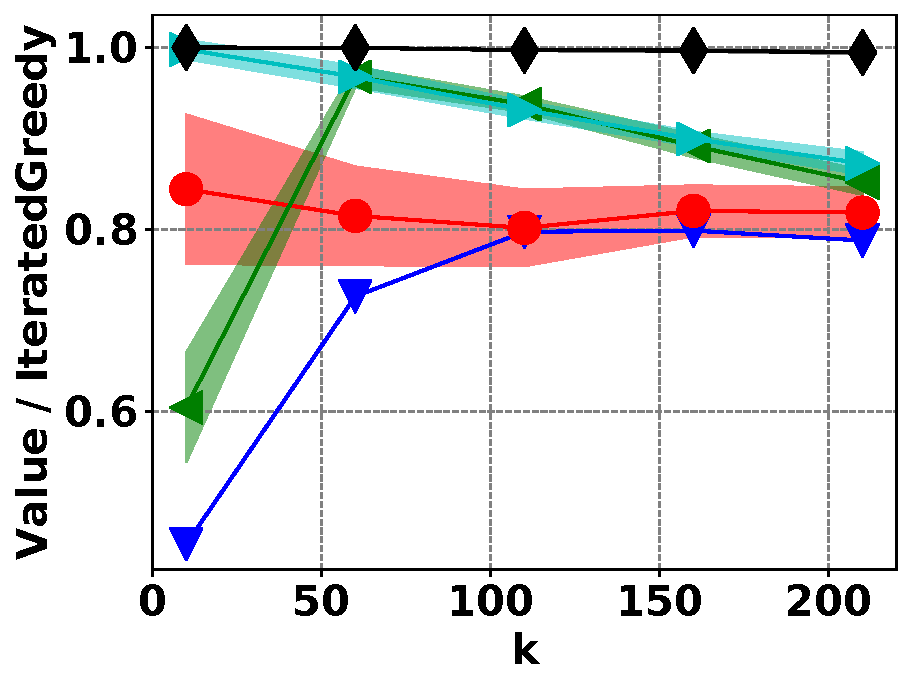
\includegraphics[width=0.28\textwidth,height=0.15\textheight]{plot/BA-val-baseline.pdf}
  }
  \subfigure[Queries, BA]{ \label{fig:query-ba}
    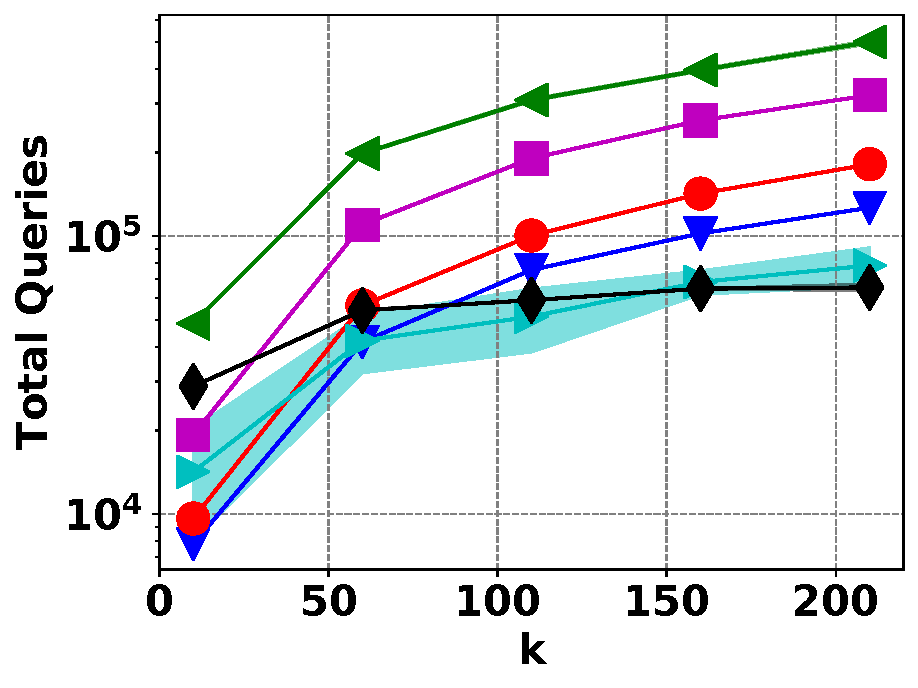
\includegraphics[width=0.28\textwidth,height=0.15\textheight]{plot/BA-query-baseline.pdf}
  }
  \subfigure[Rounds, BA]{ \label{fig:rounds-ba}
    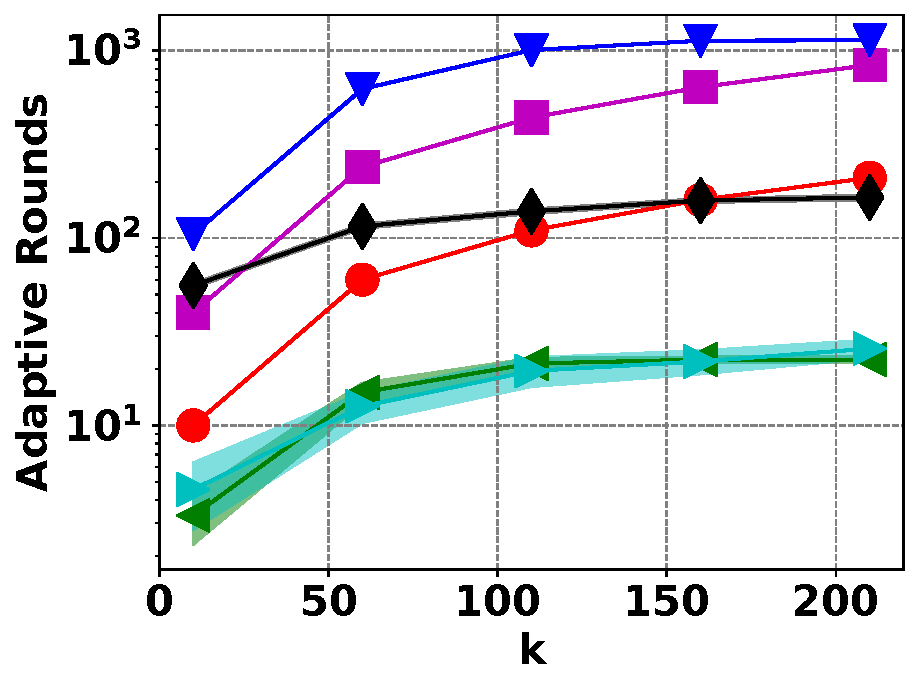
\includegraphics[width=0.28\textwidth,height=0.15\textheight]{plot/BA-round-baseline.pdf}
  }

  \subfigure[Objective, ca-GrQc]{ \label{fig:val-grqc}
    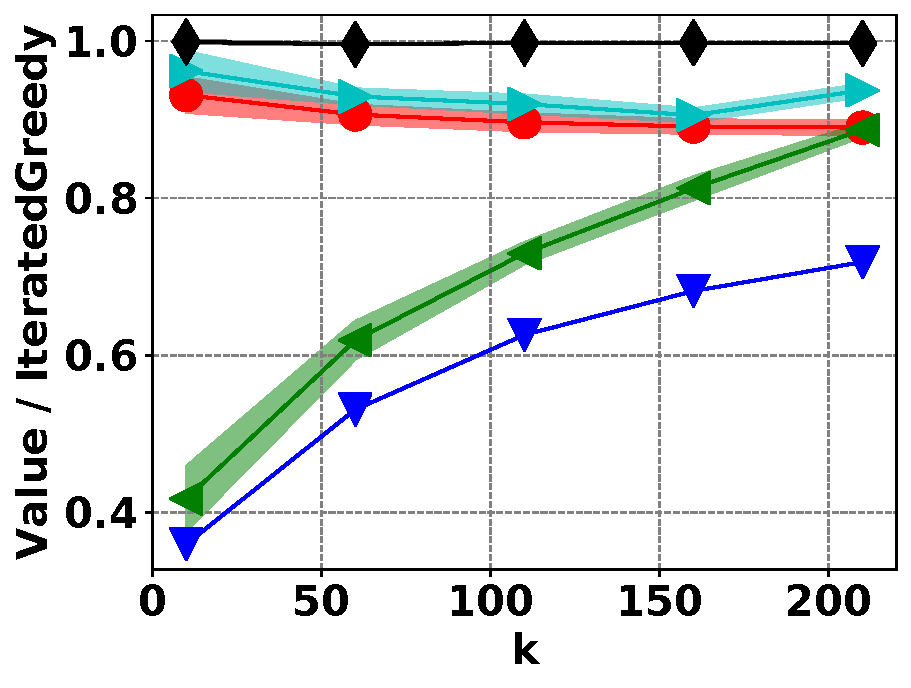
\includegraphics[width=0.28\textwidth,height=0.15\textheight]{plot/grqc-val-smallK-baseline.pdf}
  }
  \subfigure[Queries, ca-GrQc]{ \label{fig:query-grqc}
    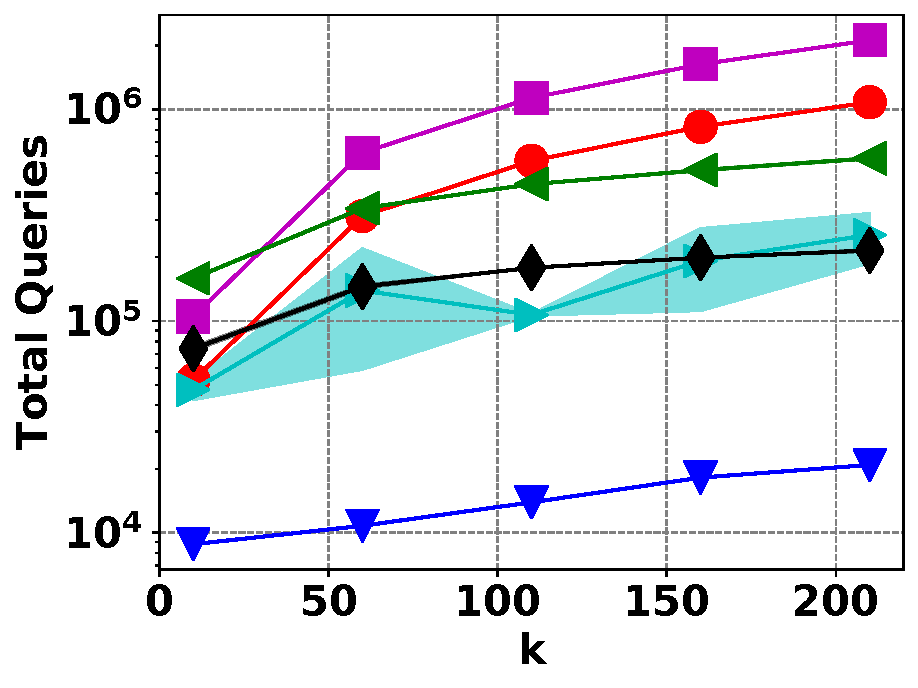
\includegraphics[width=0.32\textwidth,height=0.15\textheight]{plot/grqc-query-smallK-baseline.pdf}
  }
  \subfigure[Rounds, ca-GrQc]{ \label{fig:rounds-grqc}
    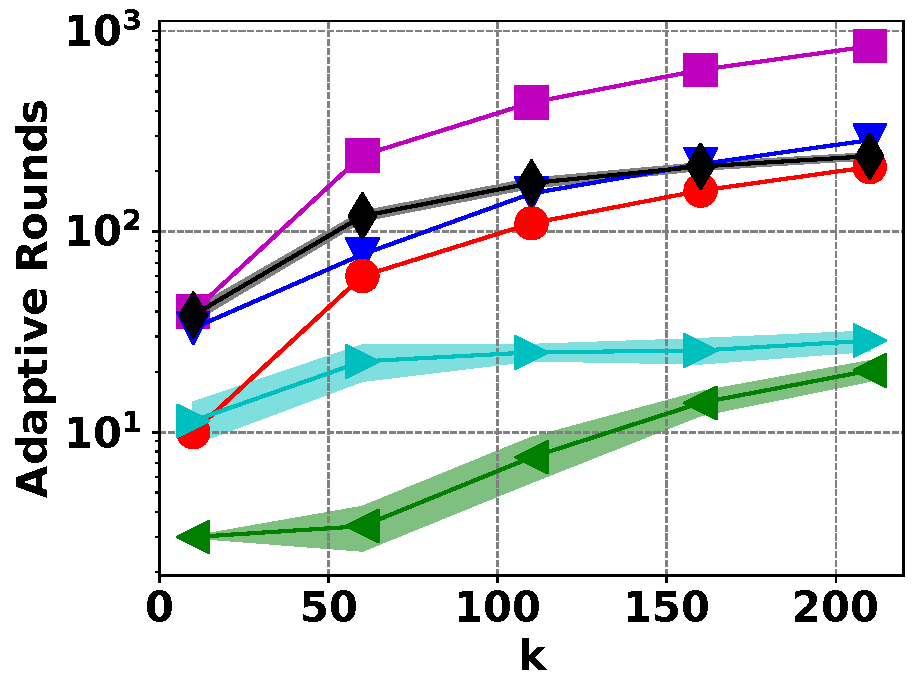
\includegraphics[width=0.32\textwidth,height=0.15\textheight]{plot/grqc-round-smallK-baseline.pdf}
  }
  \caption{Additional results for maximum cut on BA and ca-GrQc. The legend in Fig.~\ref{fig:main} applies.} 
  \label{fig:apx-exp-maxcut}
\end{figure}
\begin{figure}[ht] \centering %%TODO: remove legend from BA plots \centering
  \subfigure[Objective, small $k$]{ \label{fig:val-astro}
    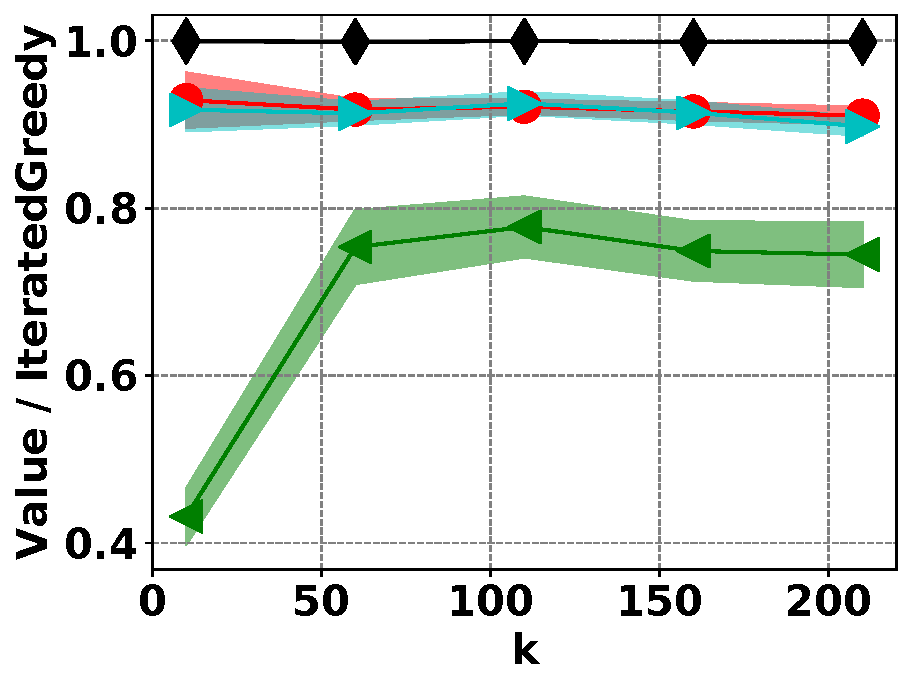
\includegraphics[width=0.28\textwidth,height=0.15\textheight]{plot/astro-val-smallK-baseline.pdf}
  }
  \subfigure[Queries, small $k$]{ \label{fig:query-astro}
    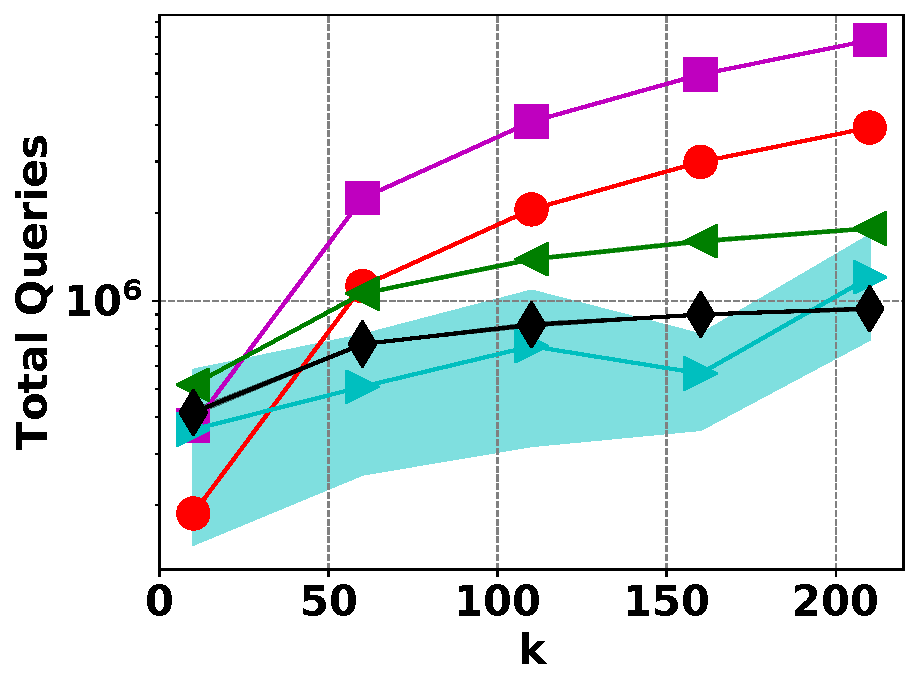
\includegraphics[width=0.28\textwidth,height=0.15\textheight]{plot/astro-query-smallK-baseline.pdf}
  }
  \subfigure[Rounds, small $k$]{ \label{fig:rounds-astro}
    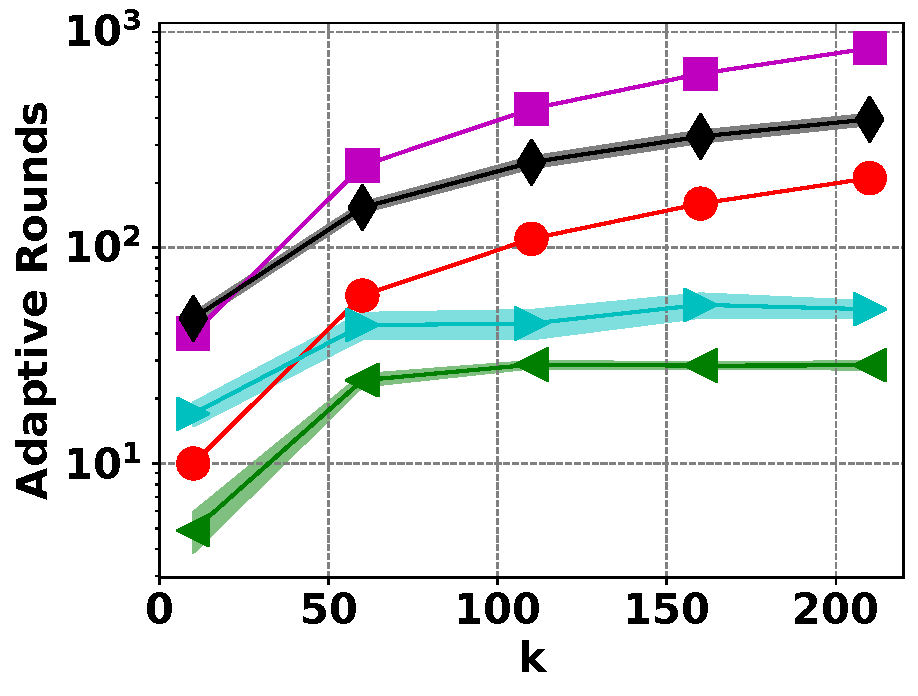
\includegraphics[width=0.28\textwidth,height=0.15\textheight]{plot/astro-round-smallK-baseline.pdf}
  }

  \subfigure[Objective, large $k$]{ \label{fig:val-astro-largek}
    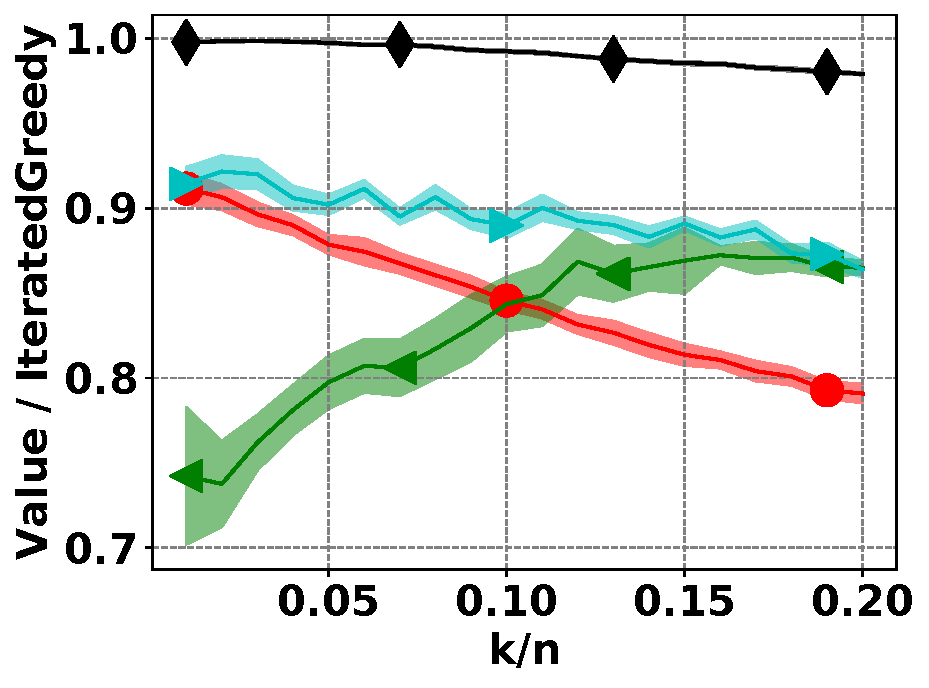
\includegraphics[width=0.28\textwidth,height=0.15\textheight]{plot/astro-val-largeK-baseline.pdf}
  }
  \subfigure[Queries, large $k$]{ \label{fig:query-astro-largek}
    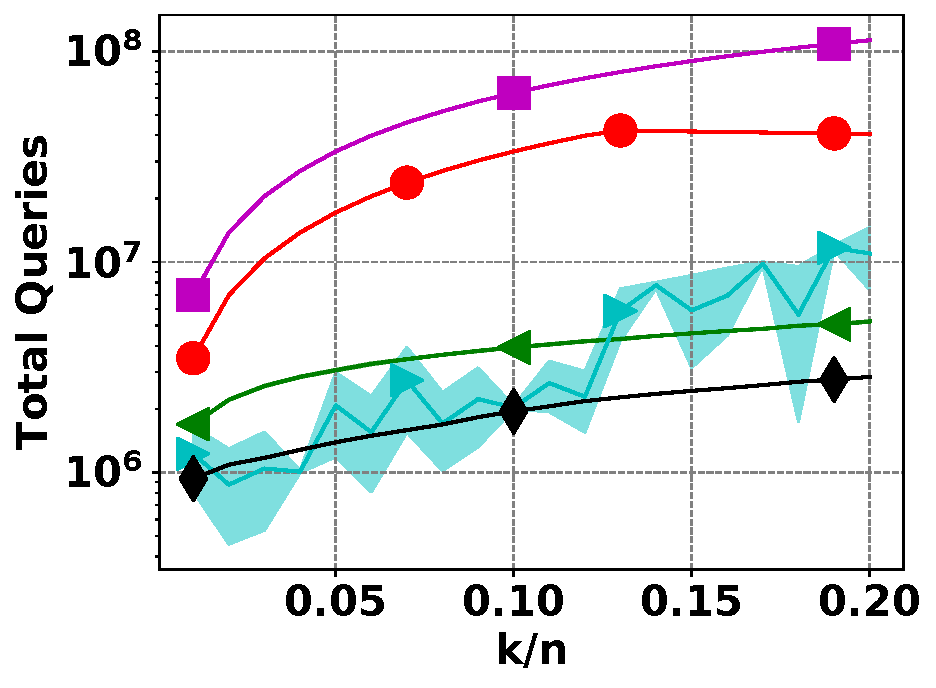
\includegraphics[width=0.28\textwidth,height=0.15\textheight]{plot/astro-query-largeK-baseline.pdf}
  }
  \subfigure[Rounds, large $k$]{ \label{fig:rounds-astro-largek}
    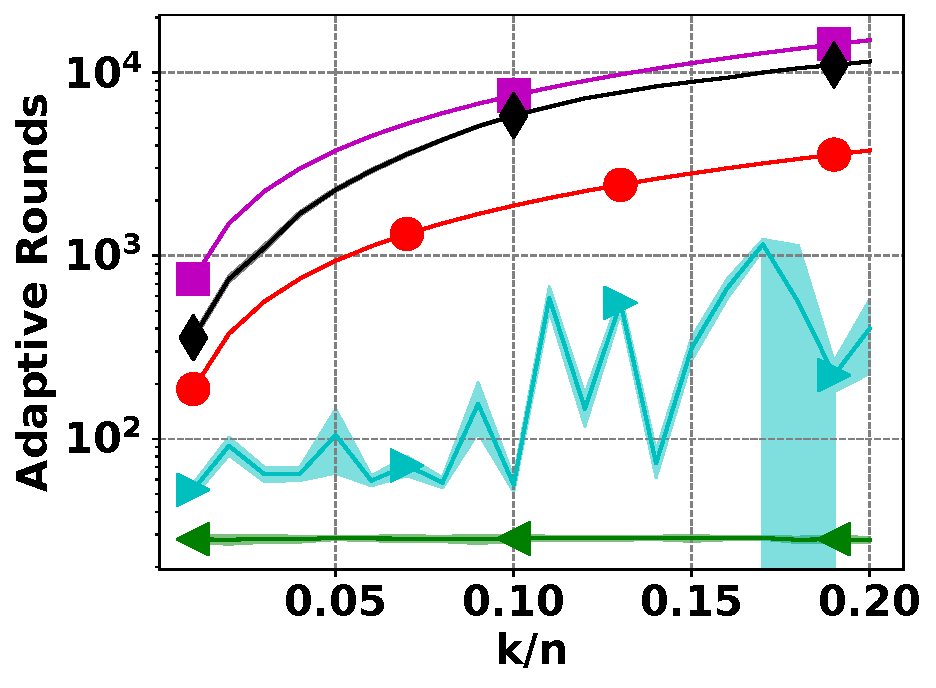
\includegraphics[width=0.28\textwidth,height=0.15\textheight]{plot/astro-round-largeK-baseline.pdf}
  }
  \caption{Results for revenue maximization on ca-Astro, for both small and large $k$ values. Large $k$ values are indicated by a fraction of the total number $n$ of nodes. The legend is the same as in Fig.~\ref{fig:main}.} 
  \label{fig:apx-exp-revmax}
\end{figure}
Results on additional datasets for the maximum cut application are
shown in Figs.~\ref{fig:apx-exp-maxcut}. 
These results are qualitatively
similar to the ones discussed in Section~\ref{sec:exp}. 
For the revenue maximization application, results on ca-Astro are shown
in Figs.~\ref{fig:apx-exp-revmax}, 
for both small and large $k$ values. These results
are qualitatively similar to the results for the maximum cut application. 
%, although
%it should be noted that the low objective value for \anm observed on small $k$ values
%in the maximum cut application extends to larger $k$ values (see Fig.~\ref{fig:val-astro-largek})
%on the revenue maximization application. 

\begin{figure*}[t] \centering
  \subfigure[Objective, BA]{ \label{fig:val-BA-2-atg}
    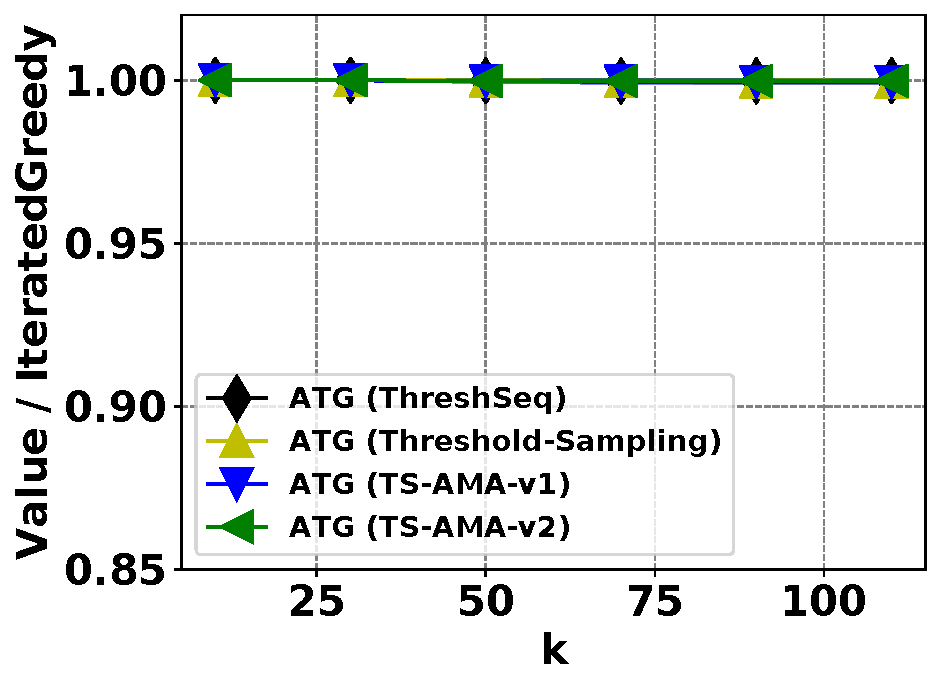
\includegraphics[width=0.3\textwidth,height=0.16\textheight]{plot/BA-val-sample-atg}
  }
  \subfigure[Rounds, BA]{ \label{fig:rounds-BA-2-atg}
    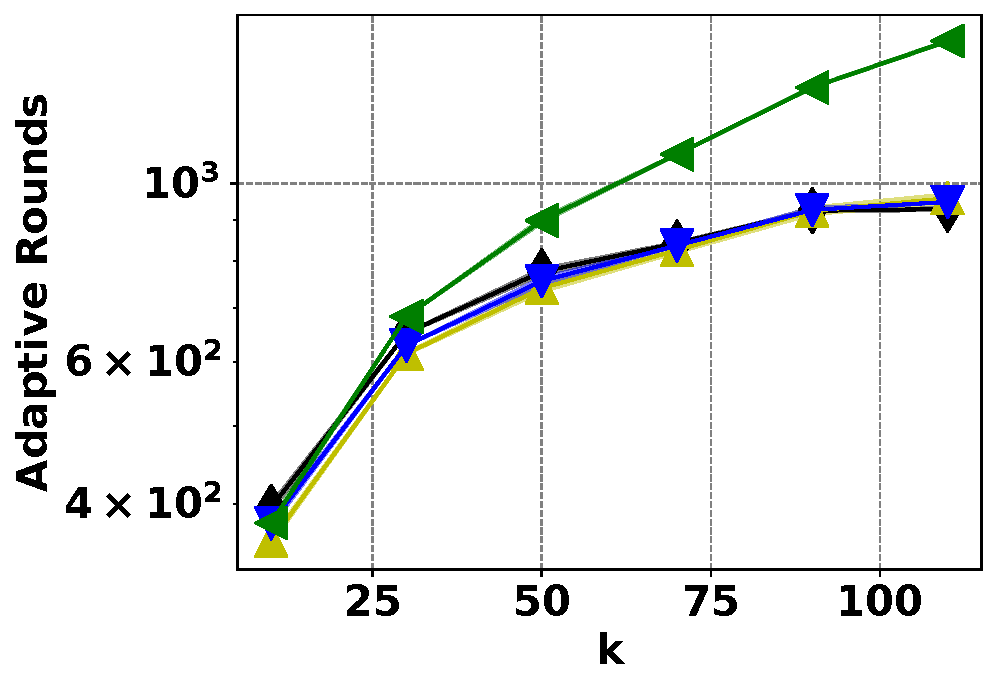
\includegraphics[width=0.3\textwidth,height=0.16\textheight]{plot/BA-round-sample-atg}
  }
  \subfigure[Queries, ca-GrQc]{ \label{fig:query-BA-2-atg}
    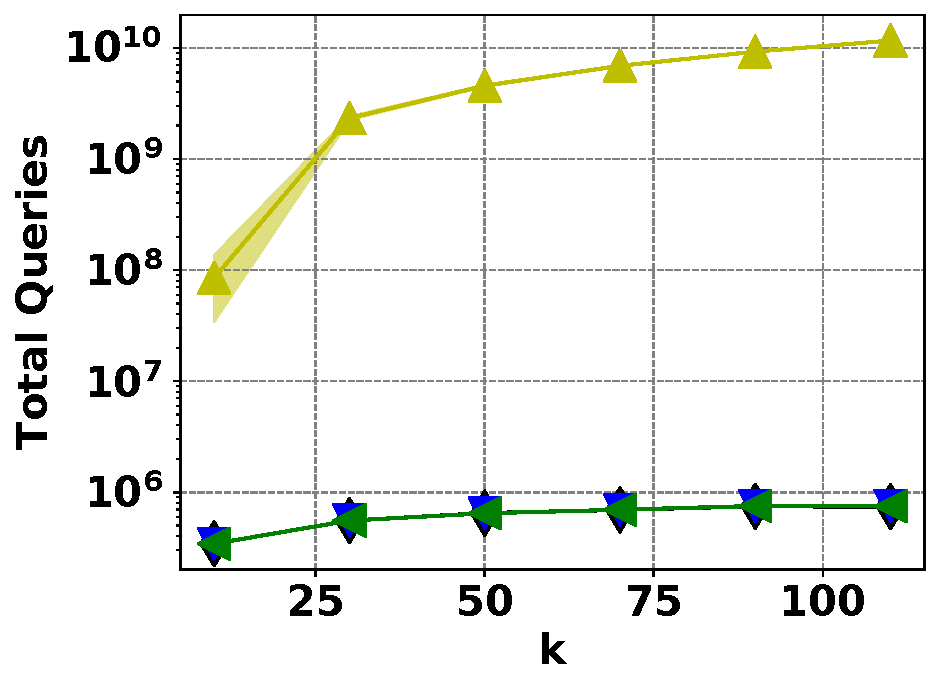
\includegraphics[width=0.3\textwidth,height=0.16\textheight]{plot/BA-query-sample-atg}
  }
  \subfigure[Objective, ca-GrQc]{ \label{fig:val-grqc-2-atg}
    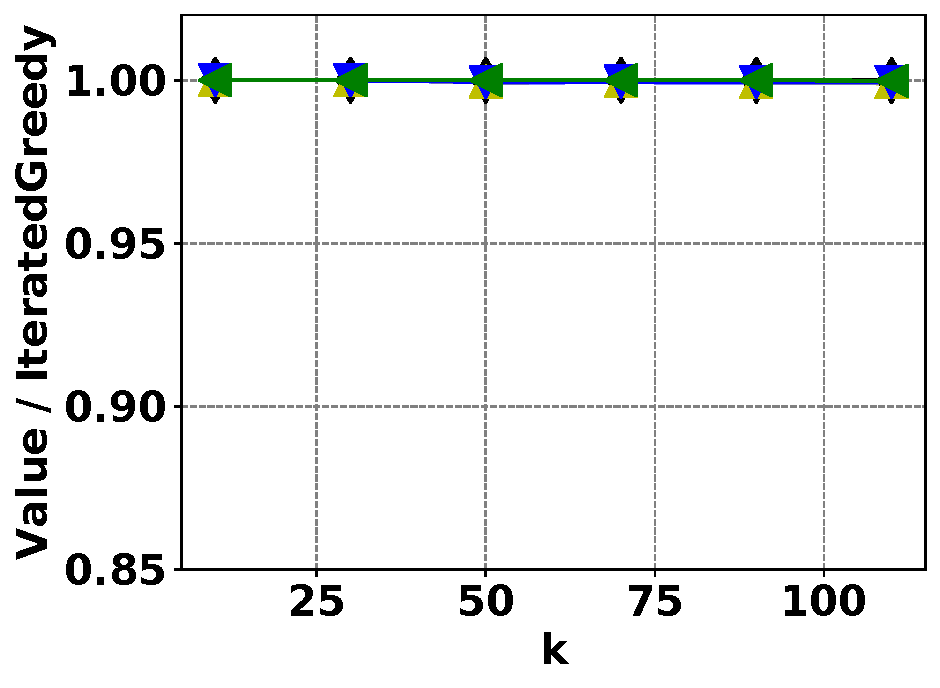
\includegraphics[width=0.3\textwidth,height=0.16\textheight]{plot/grqc-val-sample-atg}
  }
  \subfigure[Rounds, ca-GrQc]{ \label{fig:rounds-grqc-2-atg}
    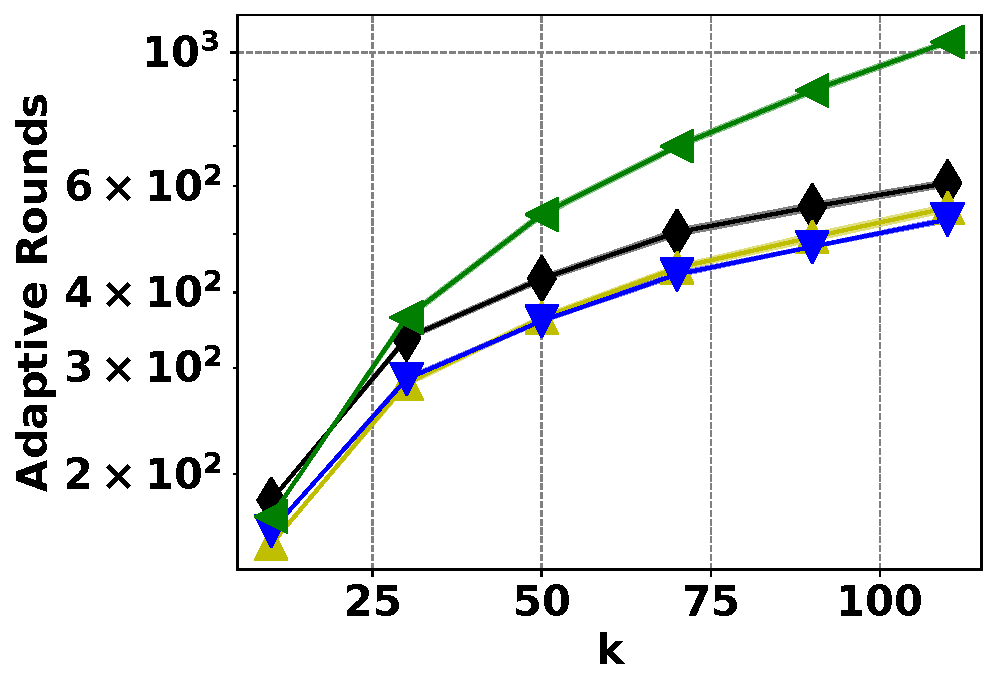
\includegraphics[width=0.3\textwidth,height=0.16\textheight]{plot/grqc-round-sample-atg}
  }
  \subfigure[Queries, ca-GrQc]{ \label{fig:query-grqc-2-atg}
    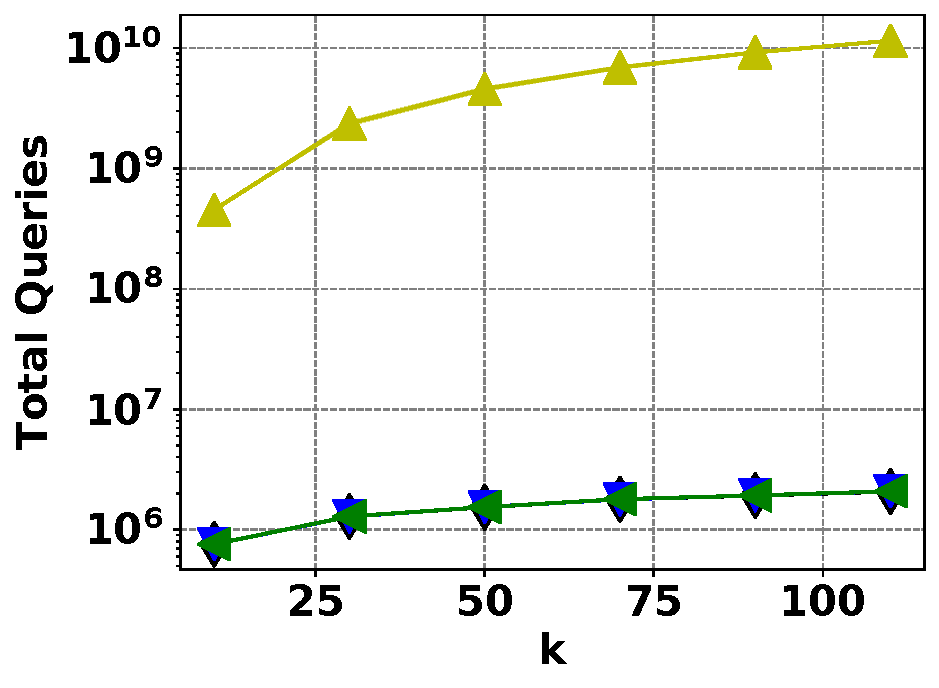
\includegraphics[width=0.3\textwidth,height=0.16\textheight]{plot/grqc-query-sample-atg}
  }
  \caption{Results of \atg and \latg with four threshold procedures on two datasets. 
  The algorithms are run strictly following pseudocode.
   } \label{fig:main3}
\end{figure*}
\textbf{Comparison of \latg with different threshold sampling procedures.}
All \latg algorithms return the competitive solutions compared with \iter;
see Figs.~\ref{fig:val-BA-2-atg} and~\ref{fig:val-grqc-2-atg}.
Since each iteration of \latg calls a threshold sampling subroutine
which is based on the solution of previous iterations and 
a slowly decreasing threshold $\tau$,
after the first filtration of the subroutine, the size of the candidate set is limited.
Thus, there is no significant difference between different {\latg}s
concerning rounds and queries.
However, there are two exceptions.
First, since \tsbin is the only one who has $\oh{\log^2(n)}$ adaptive rounds,
it still runs with more rounds; see Figs.~\ref{fig:rounds-BA-2-atg} and~\ref{fig:rounds-grqc-2-atg}.
Also, the number of queries of \latg with \thresam is significantly large
with the same reason discussed in Section~\ref{sec:exp}.

\begin{figure*}[t] \centering
  \subfigure[Objective value]{ \label{fig:val-Ene}
    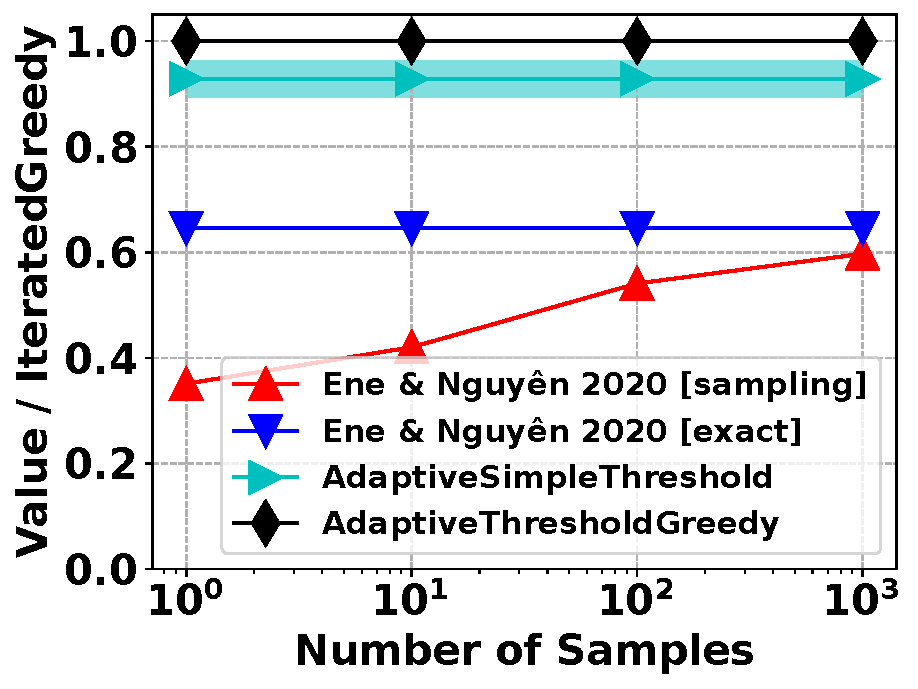
\includegraphics[width=0.28\textwidth,height=0.15\textheight]{plot/ene-val-ba.pdf}
  }
  \subfigure[Queries to set function]{ \label{fig:queryEne}
    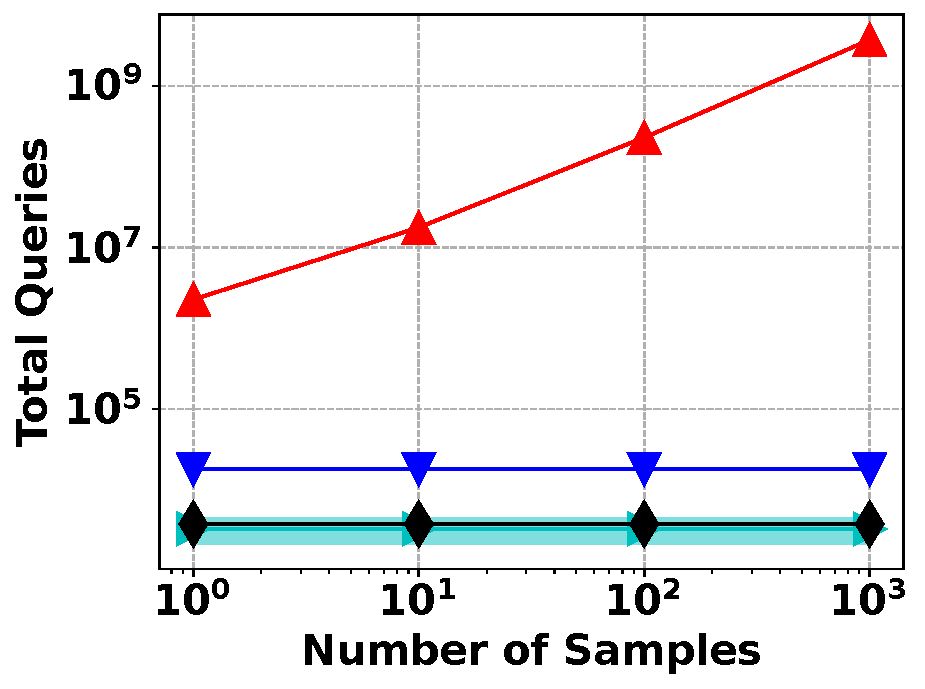
\includegraphics[width=0.28\textwidth,height=0.15\textheight]{plot/ene-query-ba.pdf}
  }
  \subfigure[Adaptive Rounds]{ \label{fig:roundsEne}
    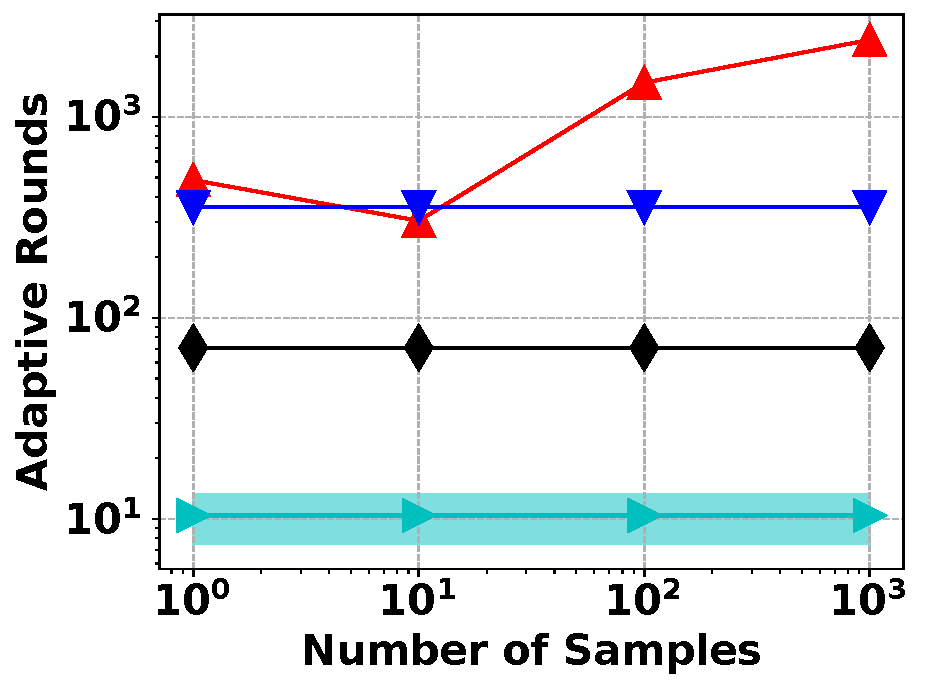
\includegraphics[width=0.28\textwidth,height=0.15\textheight]{plot/ene-rounds-ba.pdf}
  }
  \caption{Comparison of our algorithms with \shortciteS{Ene2020} on a very small random graph ($n = 87$, $k = 10$). In all plots, the $x$-axis shows the number of samples used to approximate the multilinear extension. } \label{fig:multilinear}
\end{figure*} 
\textbf{Approximation of the Multilinear Extension.}
In this section, we further investigate the performance of
\shortciteS{Ene2020} when closed-form evaluation of the multilinear
extension and its gradient are impossible. We find
that sampling to approximate the multilinear extension
and its gradient is extremely inefficient or yields poor solution
quality with a small number of samples. For this reason, we exclude
this algorithm from our revenue maximization experiments.
To perform this evaluation, we compared versions of the
algorithm of \shortciteS{Ene2020} that use varying number
of samples to approximate the multilinear extension.

Results are shown in Fig.~\ref{fig:multilinear} 
on a very small random graph with $n=87$ and $k = 10$.
The figure shows the objective value
and total queries to the set function vs. the number of samples
used to approximate the multilinear extension. 
There is a clear
tradeoff between the solution quality and the number of queries
required; at $10^3$ samples per evaluation, the algorithm
matches the objective value of the version with the 
exact oracle;
however, even at roughly $10^{11}$ queries (corresponding
to $10^4$ samples for each evaluation of the multilinear extension),
the algorithm of \shortciteS{Ene2020} is unable to exceed $0.8$ of
the IteratedGreedy value. On the other hand, if $\le 10$ samples are used to
approximate the multilinear extension, the algorithm is unable to exceed
$0.5$ of the IteratedGreedy value and still requires on the order of $10^7$
queries. 

\subsection{Further Details of Algorithm Implementations}
\label{apx:algimpl}
As stated above, we set $\epsi = 0.1$ for all algorithms
and used $100$ samples to evaluate expectations for adaptive algorithms.
Further, in the algorithms \algOnefullname, \algTwofullname, and \anm,
we ignored the smaller values of $\epsi$, $\delta$ passed to \thresam in each algorithm,
and simply used the input values of $\epsi$ and $\delta$.

For \algTwofullname, we used an early termination condition to check if the threshold
value $\tau < \opt (1 - \epsi ) / (ck)$, by using the best solution value found so far
as a lower bound on $\opt$; this early termination condition is responsible for
the high variance in total queries. We also used a sharper upper bound on $\opt / k$ in place
of the maximum singleton: the sum of the top $k$ singleton values divided by $k$. We
attempted to use the same sharper upper bound in \anm, but it resulted in signficantly worse
objective values, so we simply used the maximum singleton as described in \shortciteS{Fahrbach2018a}.

% Further, we remark that algorithms that use queries to the
% marginal gain of a function are much faster on our applications
% than algorithms that use queries of arbitrary sets. All of the algorithms
% we evaluated can be implemented to use queries of the marginal gain, except for 
% \shortciteS{Ene2020}.

\subsection{Multilinear Extension and Implementation of \shortciteS{Ene2020}} \label{apx:ene}
In this section, we describe the multilinear extension and implmentation of 
\shortciteS{Ene2020}. The multilinear extension $F$
of set function $f$ is defined to be, for $x \in [0,1]^n$:
$$ F(x) = \ex{ f(S) } = \sum_{S \subseteq V} f(S) Pr(S), $$
where $$Pr(S) = \prod_{i \in S} x_i \cdot \prod_{i \not \in S} (1 - x_i).$$
The gradient is approximated by using the central difference in each coordinate
$$ \frac{dg}{dx}(x) \approx \frac{g( x + \gamma / 2 ) - g(x - \gamma /2)}{\gamma}, $$
unless using this approximation required evaluations outside the unit cube, in which
case the forward or backward difference approximations were used. 
The parameter $\gamma$ is set to $0.5$.

Finally, for the maximum cut application, closed forms expressions exist for
both the multilinear extension and its gradient. These are:
$$ F(x) = \sum_{(u,v) \in E} x_u \cdot (1 - x_v ) + x_v \cdot (1 - x_u), $$
and
$$(\nabla F)_u  = \sum_{v \in N(u)} (1 - 2x_v). $$

\textbf{Implementation.} The algorithm was implemented as specified in the pseudocode on page
19 of the arXiv version
of \shortciteS{Ene2020}. We followed the same parameter choices as in
\shortciteS{Ene2020}, although we set $\epsi = 0.1$ as setting it to $0.05$
did not improve the objective value significantly but caused a large increase
in runtime and adaptive rounds. The value of $\delta = \epsi^3$ was used
after communications with the authors. 


\end{document}